\documentclass[11pt,oneside,a4paper]{article}
\usepackage{graphicx}
\usepackage{booktabs}
\usepackage{caption}
\usepackage{subcaption}
\usepackage{amsmath}
\usepackage{amsfonts}
\usepackage{amssymb}
\usepackage{lscape}
\usepackage{psfrag}
\usepackage[usenames]{color}
\usepackage{bbm}
\usepackage[update]{epstopdf}
\usepackage[bookmarks,pdfstartview=FitH,a4paper,pdfborder={0 0 0}]{hyperref}
\usepackage{verbatim}
\usepackage{listings}
\usepackage{textcomp}
\usepackage{fancyhdr}
\usepackage{multirow}
\usepackage{tikz}
\usepackage{lipsum}
\usepackage{xcolor}
\usepackage{wrapfig}
\usepackage[margin=1in]{geometry}
\usepackage{pdfpages}
\usepackage{ccicons}
\newcommand{\hint}[1]{{\color{blue} \em #1}}

\makeatletter
\def\cleardoublepage{\clearpage\if@twoside \ifodd\c@page\else%
\hbox{}%
\thispagestyle{empty}%
\clearpage%
\if@twocolumn\hbox{}\clearpage\fi\fi\fi}
\makeatother
\setlength\parindent{0pt}

\title{Network Security}
\author{Yannick Merkli, \texttt{ymerkli@ethz.ch}}
\date{ETH Zurich, HS 2019}

\begin{document}
	
\begin{titlepage}
\maketitle
\vspace{3cm}
\thispagestyle{empty}


\begin{abstract}
	\noindent This document is a "lecture summary" style script that closely follows the slides of the \textit{Network Security} lecture  at ETH Zurich \cite{netsec}. The contribution to this is editing and refactoring as well as providing additional material for better understanding. This summary was created during the fall semester 2019. Due to the recent update of syllabus content I believe that it is also relevant beyond that very semester.\\
	Most graphics are copy \& pasted from the slides. If you don't want yours here, please contact me and I will remove them. Otherwise, this work is published as CC BY-NC-SA.
	
	\begin{center}
		\ccbyncsa
	\end{center}
	
	\noindent I do not guarantee correctness or completeness, nor is this document endorsed by the lecturers. Feel free to point out any erratas. For the full \LaTeX \ source code, consider \texttt{\href{github.com/ymerkli/eth-summaries}{github.com/ymerkli/eth-summaries}}.\\
	
	\vspace*{1cm}
	
	\centerline{\textbf{Disclaimer: Legal use of the material}}
	\vspace*{2mm}
	
	\noindent Some knowledge, technologies, code is usable for attacks, it is illegal to use them for criminal activities. It is also illegal to make available such technologies and code without proper measures.
\end{abstract}

\end{titlepage}

\maketitle
\thispagestyle{empty}
\raggedbottom
\clearpage

\pagenumbering{roman}

\clearpage
\setcounter{tocdepth}{2}
\tableofcontents
\clearpage
\pagenumbering{arabic}


\newpage

\section{SSL, TLS, PKI}

\subsection{SSL/TLS Overview}

Goal: Secure Internet communication.\\
We need \textit{secrecy} to prevent eavesdroppers from learning sensitive information and we need entity and message authentication to prevent message alteration/ injection.

\subsection{PKI overview}

In symmetric cryptography, main challenge is key distribution as keys need to be distributed via confidential and authentic channels. In public-key systems, main challenge is key authentication (i.e., which key belongs to whom) as keys need to be distributed via authentic channels.\\
\textit{Public-key infrastructures (PKIs) provide a way to validate public keys}.\\

Terminology: 

\vspace{-\topsep}
\begin{itemize}
	\setlength{\itemsep}{0pt}
	\setlength{\parskip}{0pt}
	\item PKI: Public-key infrastructures
	\item CA: Certification authority
	\item A public-key certificate (or simply certificate) is signed and binds a name to a public key \item Trust anchor, trust root: self-signed certificates of public keys that are allowed to sign other certificates.
	\item X.509: standard format of digital certificate, defines a structure for public key certificates: Two sections: data and signature section.
\end{itemize}
\vspace{-\topsep}

Trust establishment: You cannot establish trust out of thin air - we need a root of trust to establish trust in other entities. Cryptographic operations enable transfer of trust from one entity to another.

\subsection{X.509}

X.509 defines a structure for public key certificates

\vspace{-\topsep}
\begin{itemize}
	\setlength{\itemsep}{0pt}
	\setlength{\parskip}{0pt}
	\item Two sections: data and signature sec1on
	\item A CA assigns a unique name to each user and issues a signed certificate
	\item Often name is the domain or Email address
	\item Each CA issues a certificate for those beneath it
\end{itemize}
\vspace{-\topsep}

Multi-Domain Certificates are possible and used e.g. by CDNs. Content Delivery Networks (CDN) are hosting web sites for domains and thus need a certificate to service content. CDNs are obtaining a single certificate for multiple domains.

\subsection{Compelled Certificates}

Compelled certificate: public/private key pair for law enforcement (MitM attacks on TLS) with CA certificate enabling private key to sign additional certificates. Compelled certificates carry inherent risks: Since the certificates are non-repudiable, anyone who gets hold of the second valid certificate the CA's or the government's involvement in a compelled certificate creation attack. This results in a loss of trust in the CA or the government. If the CA creates an intermediary CA certificate for the government, then that certificate would have to be registered in a CT log, but in that case, the attack
does not become directly attributable to VeriSign, as the forged certificate is signed by the intermediary certificate.

\newpage

\subsection{Approaches to improve TLS}

\subsubsection{The “Let’s Encrypt” CA}

Goal: provide free certificates with automatic domain validation, issuance, and renewal. It uses relatively short-lived certificates (90 days). It is based on ACME (Automated Certificate Management Environment).

\subsubsection{Levels of trust}

Have different levels of trust in certificates:

\vspace{-\topsep}
\begin{itemize}
	\setlength{\itemsep}{0pt}
	\setlength{\parskip}{0pt}
	\item No SSL/TLS
	\item Domain validation (DV): the domain is validated but the owner could be malicious (e.g. bad.com with certificate for bad.com)
	\item Organization validation (OV) / "High assurance": A certificate provider will issue an OV class certificate to a purchaser if the purchaser can meet two criteria: the right to administratively manage the domain name in question, and perhaps, the organization's actual existence as a legal entity. (e.g. wikipedia.org)
	\item Extended validation (EV): can be issued only by a subset of certificate authorities (CAs) and require verification of the requesting entity's legal identity before certificate issuance (e.g. credit-suisse.com). They are further displayed differently in most browsers. 
\end{itemize}
\vspace{-\topsep}

\subsubsection{HTTP Strict Transport Security (HSTS)}

Goal: allows servers to declare that their clients should only use HTTPS (for a specified period). This prevents some “downgrade”, “SSL stripping”, and “session hijacking” attacks. Browsers should automatically redirect to HTTPs or display a warning message. HSTS is implemented with an HTTPS header. Example: \texttt{Strict-Transport-Security: max-age=31536000}\\
HSTS doesn't help at all if valid bogus certificates are used.

\subsubsection{HTTP Public-Key Pinning (HPKP)}

A server implementing HPKP will provide the client with a list of hashes of valid
certificates for the domain. This list is delivered in an HTTP header that also contains a
max-age value. The client will then “pin” those hashes — subsequent connection within the
max-age period will only succeed if the certificate offered by the server matches the pinned
hashes for that domain. A MitM with a different certificate would therefore fail. Example:\\
\hspace*{5mm} \texttt{Public-Key-Pins: max-age=2592000; pin-sha256="..."; pin-sha256="...";\\
\hspace*{5mm} report-uri="...";\\
}
MiTM attacks can still succeed even with HPKP: HPKP is TOFU (Trust On First Use). If the first policy received comes from an
attacker, the browser will be happy to communicate with the bogus website and will block
the legitimate server. Also if a weak hash function is used, the attacker could generate a
certificate with a colliding hash — but in that case HPKP would be the last of our problems.\\

Further problem with HPKP: certificates can change often (e.g with Let's encrypt). If a certificate changes but users still hold the old policy (since the max-age hasn't expired yet), clients won't accept the new certificate although it is legitimate.

\newpage

\subsubsection{Certificate revocation}

Certificate revocation is a mechanism to invalidate certificates (e.g. after a private key is disclosed or after a trusted employee leaves a company). CA periodically publishes certificate revocation List (CRL).\\
Problem: CAP theorem (Consistency, Availability, tolerance to Par11on):
impossible to achieve all 3, need to sacrifice one!

\subsubsection{Online Certificate Status Protocol (OCSP)}

Online Certificate Status Protocol (OCSP) to verify certificate status, ensure certificate is valid and has not been revoked. Browsers will send certs to OCSP server for verification.\\
Problem: 
\vspace{-\topsep}
\begin{itemize}
	\setlength{\itemsep}{0pt}
	\setlength{\parskip}{0pt}
	\item “Optimistic” treatment of OCSP failure information: If OCSP server does not respond, a certificate would be considered invalid, although the certificate most likely isn't. This leads to false positives, which is annoying for browser users, that's why most browsers don't treat a non-responding OCSP server as invalid certificate.
	\item OCSP servers can be slow, which is another reason for browsers to deactivate it by default, since users otherwise may switch browsers.
	\item OCSP can leak browsing information outside of private browsing mode as Microsoft’s CryptoAPI and Apple’s Security Framework API cache OCSP responses in OS.
\end{itemize}
\vspace{-\topsep} 

Possible solution: OCSP stapling allows the presenter of a certificate to bear the resource cost involved in providing OCSP responses by appending ("stapling") a time-stamped OCSP response signed by the CA to the initial TLS handshake, eliminating the need for clients to contact the CA, with the aim of improving both security and performance.

\subsubsection{DNS-Based Authentica1on of Named Entities (DANE)}

Goal: authenticate TLS servers without a certificate authority (CA). DANE uses DNSSEC to bind certificates to names. Problem: this is heavily reliant on DNSSEC.

\subsubsection{Attack-resilient PKI (ARPKI)}

Goal: reduce trust in any single component (e.g. CA, log server, etc.). Reduce attack surface, no single point of failure.\\
ARPKI has a set of entities that audit each other's operation and disseminate misbehavior if detected:

\vspace{-\topsep}
\begin{itemize}
	\setlength{\itemsep}{0pt}
	\setlength{\parskip}{0pt}
	\item Client (browser) establishes TLS connections with	Domain
	\item Integrity Log Server (ILS) logs domains’ certificates, makes logs publicly available and maintains Integrity Tree
	\item Certification Authority (CA) certifies domains’ public keys, download ILS data and check consistency and check behavior of other CAs.
\end{itemize}
\vspace{-\topsep}

ARPKI communication flows:

\vspace{-\topsep}
\begin{itemize}
	\setlength{\itemsep}{0pt}
	\setlength{\parskip}{0pt}
	\item Domains obtain certificate with multiple signatures from different CAs
	\item CAs also act as validators to survey operation by ILSes. They download accepted requests and validate log
	\item $n$ parties are needed for valid certificate (ILS and $n-1$ parties are different CAs)
\end{itemize}
\vspace{-\topsep}

\begin{figure}[t!]
	\centering
	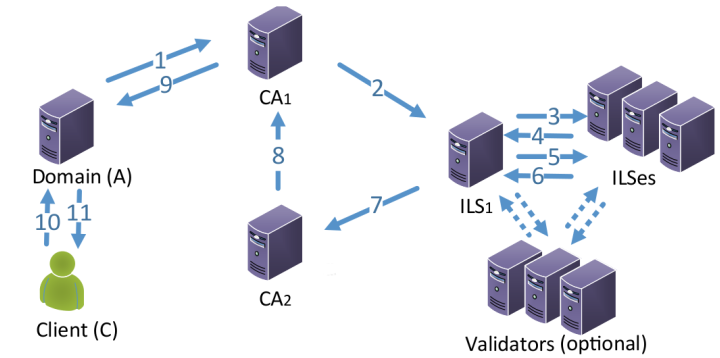
\includegraphics[width=0.5\linewidth]{figures/arpki}
	\caption{ARPKI}
	\label{fig:arpki}
\end{figure}

\newpage

\subsubsection{Certificate transparency (CT)}

Certificate	Transparency will make all public end-entity TLS certificates public knowledge,	and	will hold CAs publicly accountable for all certificates they issue. And it will do so without introducing another trusted third party.\\
CT uses a CT log that is an append-only list of certificates. The log server verifies the certificate chain (CA attribution for certificate miss-issuance and spam control). Periodically, all new certificates are appended to the append-only log and that list is then signed. All updates of the signed list of certificates ("the log") are published to the world. The CT log is implemented as a merkle hash tree. We have three participants in the protocol:

\begin{figure}
	\centering
	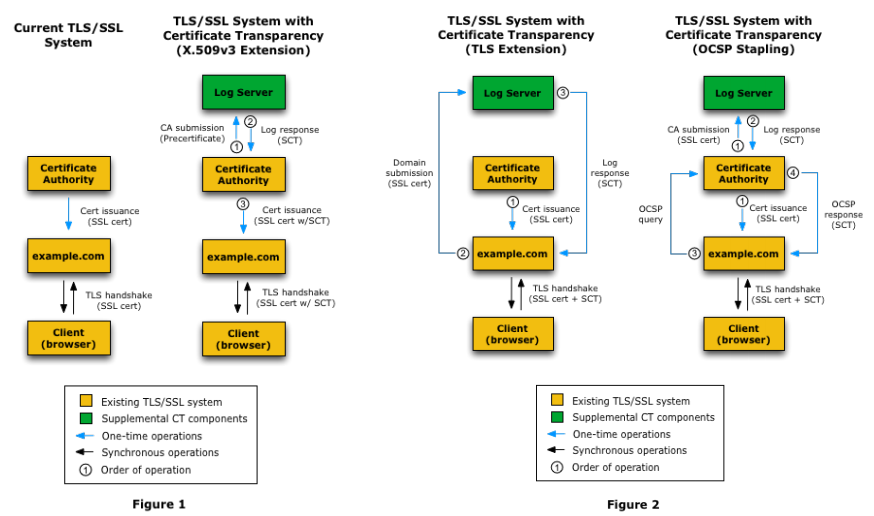
\includegraphics[width=0.9\linewidth]{figures/tls_with_ct}
	\caption{TLS with certificate transparency}
	\label{fig:tlswithct}
\end{figure}


\vspace{-\topsep}
\begin{itemize}
	\setlength{\itemsep}{0pt}
	\setlength{\parskip}{0pt}
	\item Log Server. Contains a list of certificates that is publicly available. Must
	add the certificates submitted by the CAs.
	\item Clients (auditors). Can verify the existence of certificates by checking the log server,
	and exchange information with the monitors about the log server status, in order to
	ensure the log server is not compromised.
	\item CAs (monitors). Request the addition of every newly issued cert, check that the log
	server actually adds the certificates, monitor what the other CAs are doing.
	\item Certificate owners: Query monitors to verify that nobody has logged illegitimate certs for their domain.
\end{itemize}
\vspace{-\topsep}

\newpage

Upon receiving a new certificate chain from domain or CA: the log verifies the certificate, issues a signed certificate timestamp (SCT) and promises to add the new certificate to the MHT (SCT is necessary since certs are only periodically added to log).\\
How does CT handle revocation? The certificates stay on the log forever: Merkle trees allow for easy insertion but not for immediate deletion. The current system implements revocation transparency, which is very similar to CT, but for revocation requests.\\

Disadvantages of CT:

\vspace{-\topsep}
\begin{itemize}
	\setlength{\itemsep}{0pt}
	\setlength{\parskip}{0pt}
	\item MitM attack still proceeds (but can be detected externally)
	\item Browser still needs to contact Log eventually to verify that certificate is listed in log
	\item Malicious Log server can add bogus certificate
\end{itemize}
\vspace{-\topsep}

\begin{figure}[hb]
	\centering
	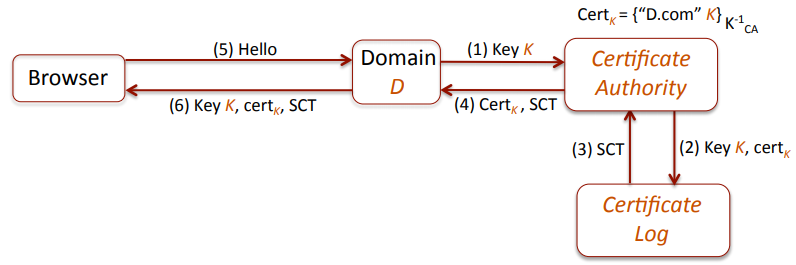
\includegraphics[width=0.6\linewidth]{figures/ct_summary}
	\caption{CT summary}
	\label{fig:ctsummary}
\end{figure}

\begin{figure}[hb]
	\centering
	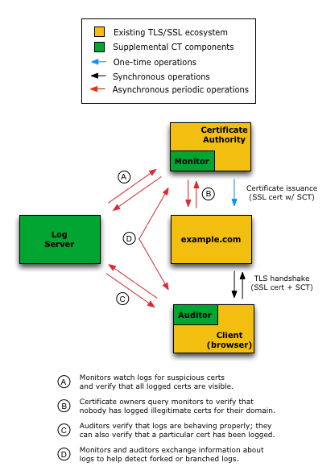
\includegraphics[width=0.5\linewidth]{figures/ct_participants}
	\caption{CT participants}
	\label{fig:ctparticipants}
\end{figure}



\newpage

\section{TLS}

Perfect forward secrecy: when obtaining a private key, I can only decrypt future sessions, not past ones.

\subsection{Cipher suites}

\texttt{TLS\_\{KEY\_EXCHANGE\}\_\{AUTHENTICATION\}\_WITH\_\{BULK\_ENCRYPTION\}\_\{MAC\}}

Example: \texttt{TLS\_DHE\_RSA\_WITH\_AES\_128\_GCM\_SHA256}\\
Key exchange: Ephemeral Diffie-Hellman, Authentication: RSA, Encryption: 128-bit AES GCM mode, MAC: 256-bit SHA-2

\subsection{Handshake protocol}

\vspace{-\topsep}
\begin{itemize}
	\setlength{\itemsep}{0pt}
	\setlength{\parskip}{0pt}
	\item Establishes keys needed by the Record Protocol, via establishment of the TLS mastersecret and subsequent key derivation.
	\item Provides authentication of server (usually) and client (rarely), using public key cryptography supported by digital certificates or pre-shared key (less common, used in IoT).
	\item Protects negotiation of all cryptographic parameters. SSL/TLS version number, encryption and hash algorithms, authentication and key establishment methods. This prevents version rollback and cipher suite downgrade attacks.
\end{itemize}
\vspace{-\topsep}

\begin{figure}[hb]
	\centering
	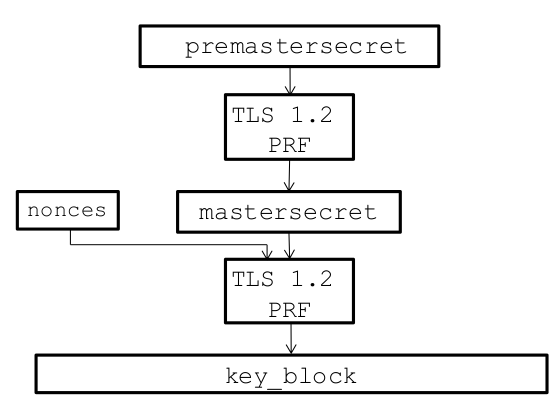
\includegraphics[width=0.4\linewidth]{figures/tls_key_derivation}
	\caption{TLS key derivation. The premastersecret is either a client-generated random-value (RSA) or the negotiated DH shared secret (DH). Nonces are public. All symmetric keys come from the key\_block (48 bytes). The split of the key\_block depends on the cipher suite.}
	\label{fig:tlskeyderivation}
\end{figure}


\subsubsection{Key establishment options}

\vspace{-\topsep}
\begin{itemize}
	\setlength{\itemsep}{0pt}
	\setlength{\parskip}{0pt}
	\item RSA: RSA key generation is expensive, that's why keys are reused. Thus, RSA does not provide perfect forward secrecy.
	\item Static Diffie-Hellman: Server certificate contains DH parameters (group, generator g)
	and static DH value $g^x$. Client chooses y, computes $g^y$ and sends to server. $$premastersecret = g^{xy}$$
	Thus, Static Diffie-Hellman does not provide perfect forward secrecy.
	\item Anonymous Diffie-Hellman: Each side sends Diffie-Hellman values in group chosen by
	server, but no authentication of these values. Vulnerable to man-in-middle attacks even if only offered.
	\item The key exchange is called “ephemeral” if the client and server both choose a new key pair for every exchange. Ephemeral key exchanges offer PFS.
	\item (EC)DHE: Offers perfect forward secrecy.
\end{itemize}
\vspace{-\topsep}

\newpage

\subsection{Record protocol}

TLS Record Protocol uses symmetric encryption, using the keys negotiated during the handshake protocol. It provides:

\vspace{-\topsep}
\begin{itemize}
	\setlength{\itemsep}{0pt}
	\setlength{\parskip}{0pt}
	\item Data origin authentication, integrity using a MAC.
	\item Confidentiality using a symmetric encryption algorithm.
	\item Anti-replay using sequence numbers protected by the MAC.
	\item Optional compression.
	\item A stream-oriented API for applications making use of it.
	\item Hence TLS may fragment into smaller records or coalesce into larger records any data supplied by the calling application.
\end{itemize}
\vspace{-\topsep}

Different record layer encryption schemes:

\vspace{-\topsep}
\begin{itemize}
	\setlength{\itemsep}{0pt}
	\setlength{\parskip}{0pt}
	\item AES is secure in both 128-bit and 256-bit mode (and more), however if CBC mode is used, padding oracle attacks are possible. GCM mode is secure.
	\item DES is not secure.
	\item RC4 is not secure (see \ref{attack_on_rc4})
\end{itemize}
\vspace{-\topsep}

The TLS record protocol uses MAC-then-encrypt: this is \textit{really really bad} since this opens up the possibility of padding oracle attacks!

\begin{figure}[hb]
	\centering
	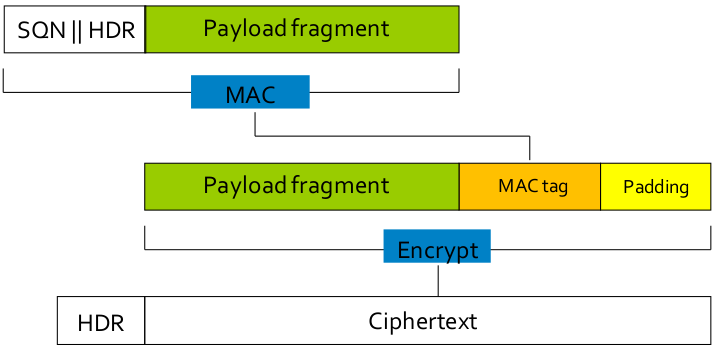
\includegraphics[width=0.4\linewidth]{figures/tls_record_protocol}
	\caption{TLS Record Protocol: MAC-Encode-Encrypt}
	\label{fig:tlsrecordprotocol}
\end{figure}

\subsubsection{TLS Record Protocol Sequence Numbers}

When the handshake is done, both client and server set the sequence number to 0 and start counting. Sequence number is 64 bits in size and is incremented for each new message. Once we reach the top (overflow), we throw away the keys and rerun the handshake (however this will rarely happen.. $2^{64}$ is very large).\\
Server and client both each maintain a copy of two seq. numbers: one for sending, one for receiving. Sequence numbers are not transmitted as part of message (TCP already provides reliable transport), however they are included in the MAC. Sequence numbers and MAC together give replay protection.\\
A wrong sequence number leads to a failure of the MAC verification. TLS is thus reliant on TCP to deliver messages in order.


\newpage

\section{Attacks against TLS}

\subsection{Attack on RC4}
\label{attack_on_rc4}

In RC4, we have biases towards certain byte values in the first 256 bytes of the RC4 cipher outputs. For example, at position 16, byte 240 is much more likely.\\
By analyzing \textbf{many} ciphertexts, we can do bayesian analysis and check which byte was most likely at each position. This then allows to recover the plaintext. For example, we could analyze the values at position 16 and XOR the most likely value with 240, which gives the plaintext.\\
An example on how to exploit this is: You want to target a secure cookie in the HTTPS session between a client running a web browser B and a web server W . You know W serves secure cookies over HTTPS, and you control a second web server, E, the client visits. The client will run javascript code served from E. While this code cannot directly access cookies from W (due to the same-origin policy, SOP), it can make requests to W : the cookies will be automatically attached by the browser to the new requests. The javascript can repeat enough requests to make the attack succeed — allowing the attacker to recover the plaintext cookie.

\subsection{FREAK attack}

\begin{figure}[hb]
	\centering
	\begin{subfigure}[t]{.5\textwidth}
		\centering
		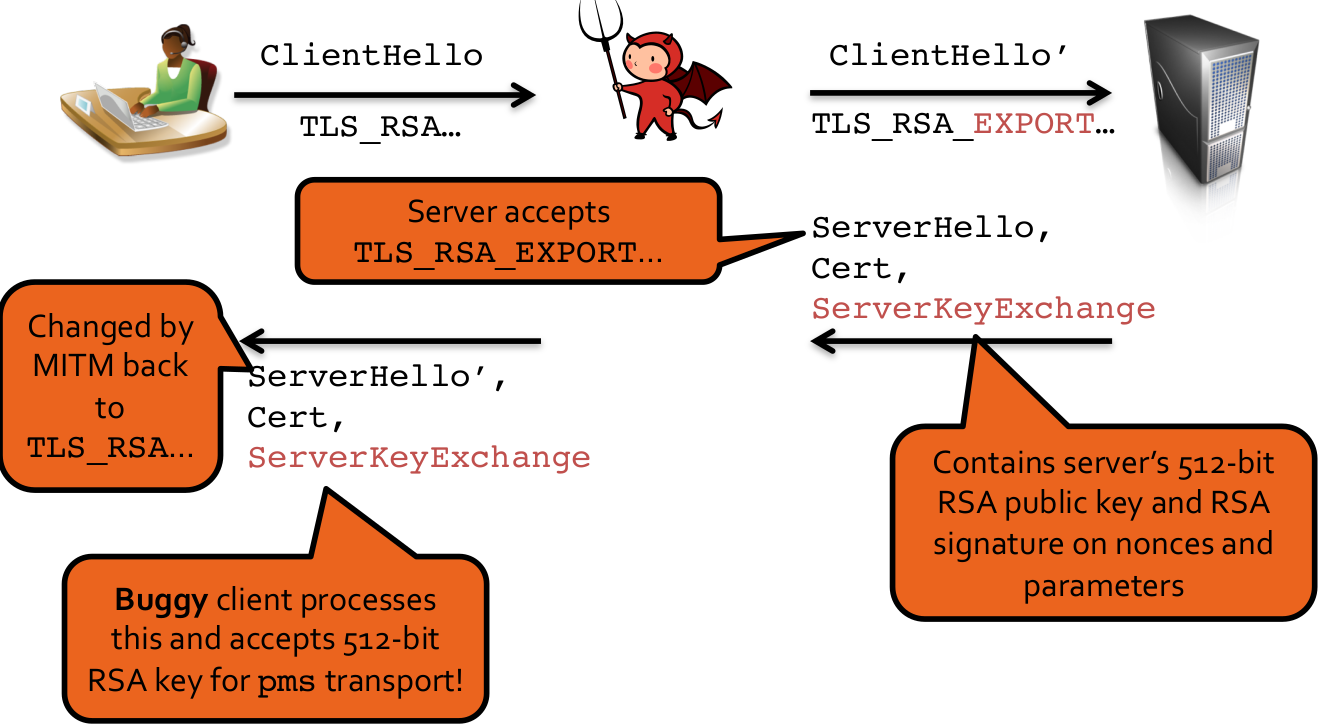
\includegraphics[width=\linewidth]{figures/tls_freak_1}
		\label{fig:tls_freak_1}
	\end{subfigure}%
	\begin{subfigure}[t]{.5\textwidth}
		\centering
		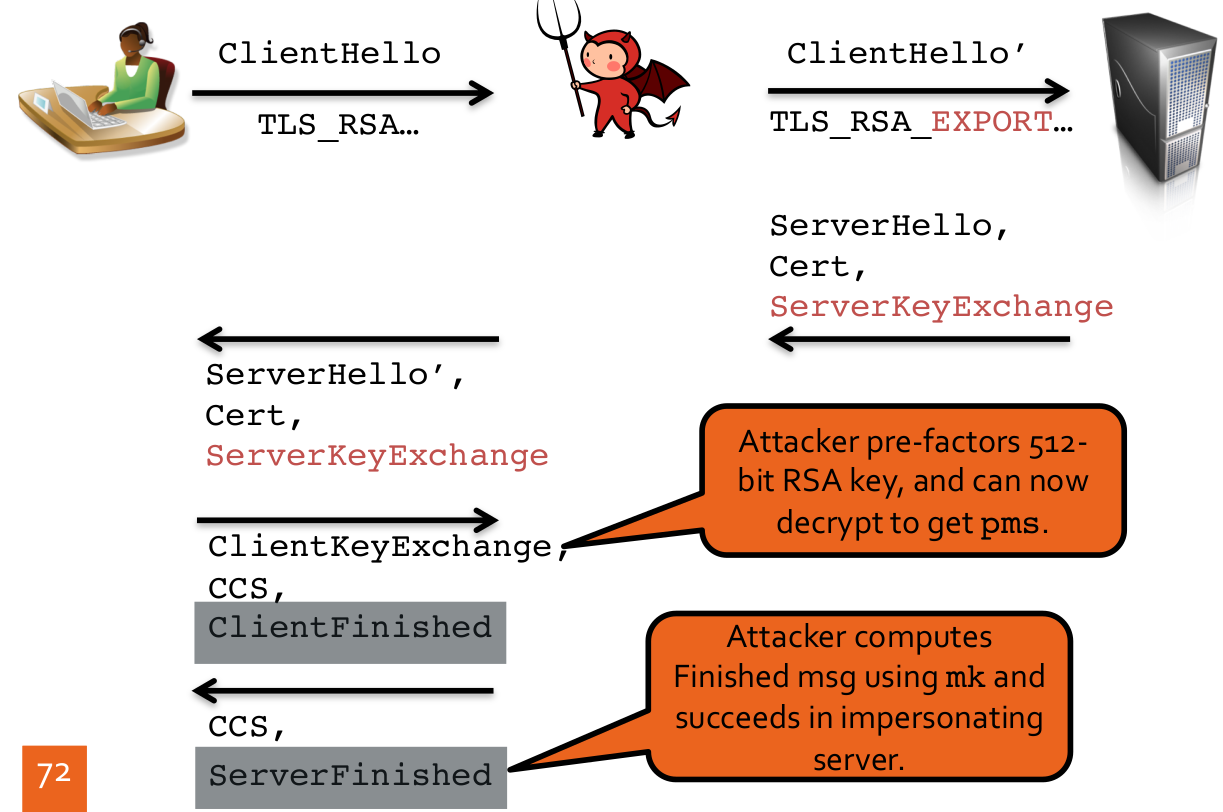
\includegraphics[width=\linewidth]{figures/tls_freak_2}
		\label{fig:tls_freak_2}
	\end{subfigure}
\end{figure}

In a FREAK attack, an active MiTM attacker forces a TLS session to use insecure export ciphers. Export ciphers are intentionally weak ciphers that were offered by the US in the 90s. During that time, these ciphers were only breakable with huge resources and a large budget. Today, they are breakable with 100\$ of AWS credit.\\
The active MiTM attacker alters the unencrypted ClientHello message to request Export RSA as the
cipher suite. Similarly, ServerHello message is changed to reflect the original ClientHello. The ServerFinished message also needs to reflect the original ClientHello and ServerHello, with the unchanged cipher suite, otherwise the client would fail transcript verification.\\
The attacker needs to be able to pre-factor the RSA key, (or factor an on-the-fly RSA key “in real time”) and craft a new ServerFinished message, removing the original from the communication channel. Since servers reuse RSA keys, the attacker can just connect to the server in advance and factor the key. Once the attacker has the key, she can decrypt the pre-mastersecret and then generate the mastersecret, using the nonces (which are in plaintext, thus public).\\
This attack was only possible due to buggy TLS client: when requesting export RSA, the server responds with a ServerKeyExchange message which contain the RSA pubKey and RSA signatures on nonces and parameters. For normal RSA (which the client thinks he's using) we would not get this message. Buggy TLS client accepted the weak key and used it, even though a different cipher was requested.\\
FREAK requires an active MiTM. The attacker needs to keep impersonating the server for all new sessions or for possible future CCS+Finish.

\subsection{Heartbleed}

The Heartbeet protocol of TLS is equivalent to ping (icmp), just for TLS. You send a msg to a server, server sends the exact msg back. Turns out, OpenSSL didn't do proper bound checking on the received msg. If you send a short msg but tell the server it's a long message, the server would send a long msg. The server would then just read over the buffer and read into memory. By doing this over and over (and being lucky) you could receive sensitive data such as passwords or private keys.

\subsection{Apple \texttt{goto fail}}

\begin{figure}[hb]
	\centering
	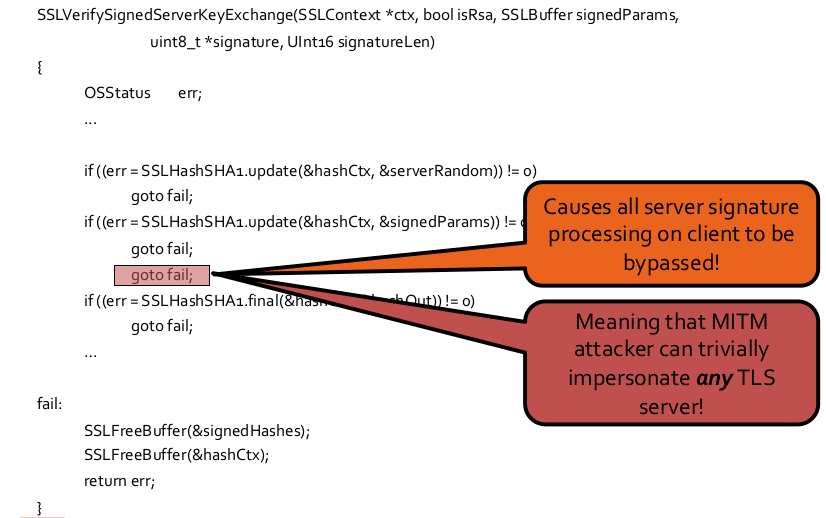
\includegraphics[width=0.5\linewidth]{figures/apple_goto_fail}
	\caption{Apple goto fail in iPhone and Mac TLS library}
	\label{fig:applegotofail}
\end{figure}

\section{TLS 1.3}

Main objectives of TLS 1.3:

\vspace{-\topsep}
\begin{itemize}
	\setlength{\itemsep}{0pt}
	\setlength{\parskip}{0pt}
	\item Protocol simplification (reducing options and removing broken cipher suites).
	\item Reduce latency of initial secure data communication (1-RTT and 0-RTT for resumed sessions).
	\item Improve security and privacy.
	\item Remove compression, RC4, MAC-then-Encrypt, RSA key transport,	custom DH and ECDH groups, renegotiation.
	\item A stream-oriented API for applications making use of it.
	\item Hence TLS may fragment into smaller records or coalesce into larger records any data supplied by the calling application.
\end{itemize}
\vspace{-\topsep}

\subsection{TLS 1.3 1-RTT handshake}

Basic idea: client sends Hello message which already includes its DH pubKey $g^x$. For this to work, the client needs to guess which DH groups the server supports.
Assuming the server actually supports the DH group it sends a ServerHello with the server DH pubKey AND it can already encrypt data since the server knows the nonces and both DH values.
DH and ECDH groups: A limited set of DH and ECDH groups are supported in TLS 1.3. This reduces likelihood of fall-back to 2-RTT and removes complexity from implementations.

\subsection{TLS 1.3 - Resumption}

Resumption uses pre-shared keys (PSK) which were established in prior session. The client sends a list of PSK IDs, one of which is selected by the server.

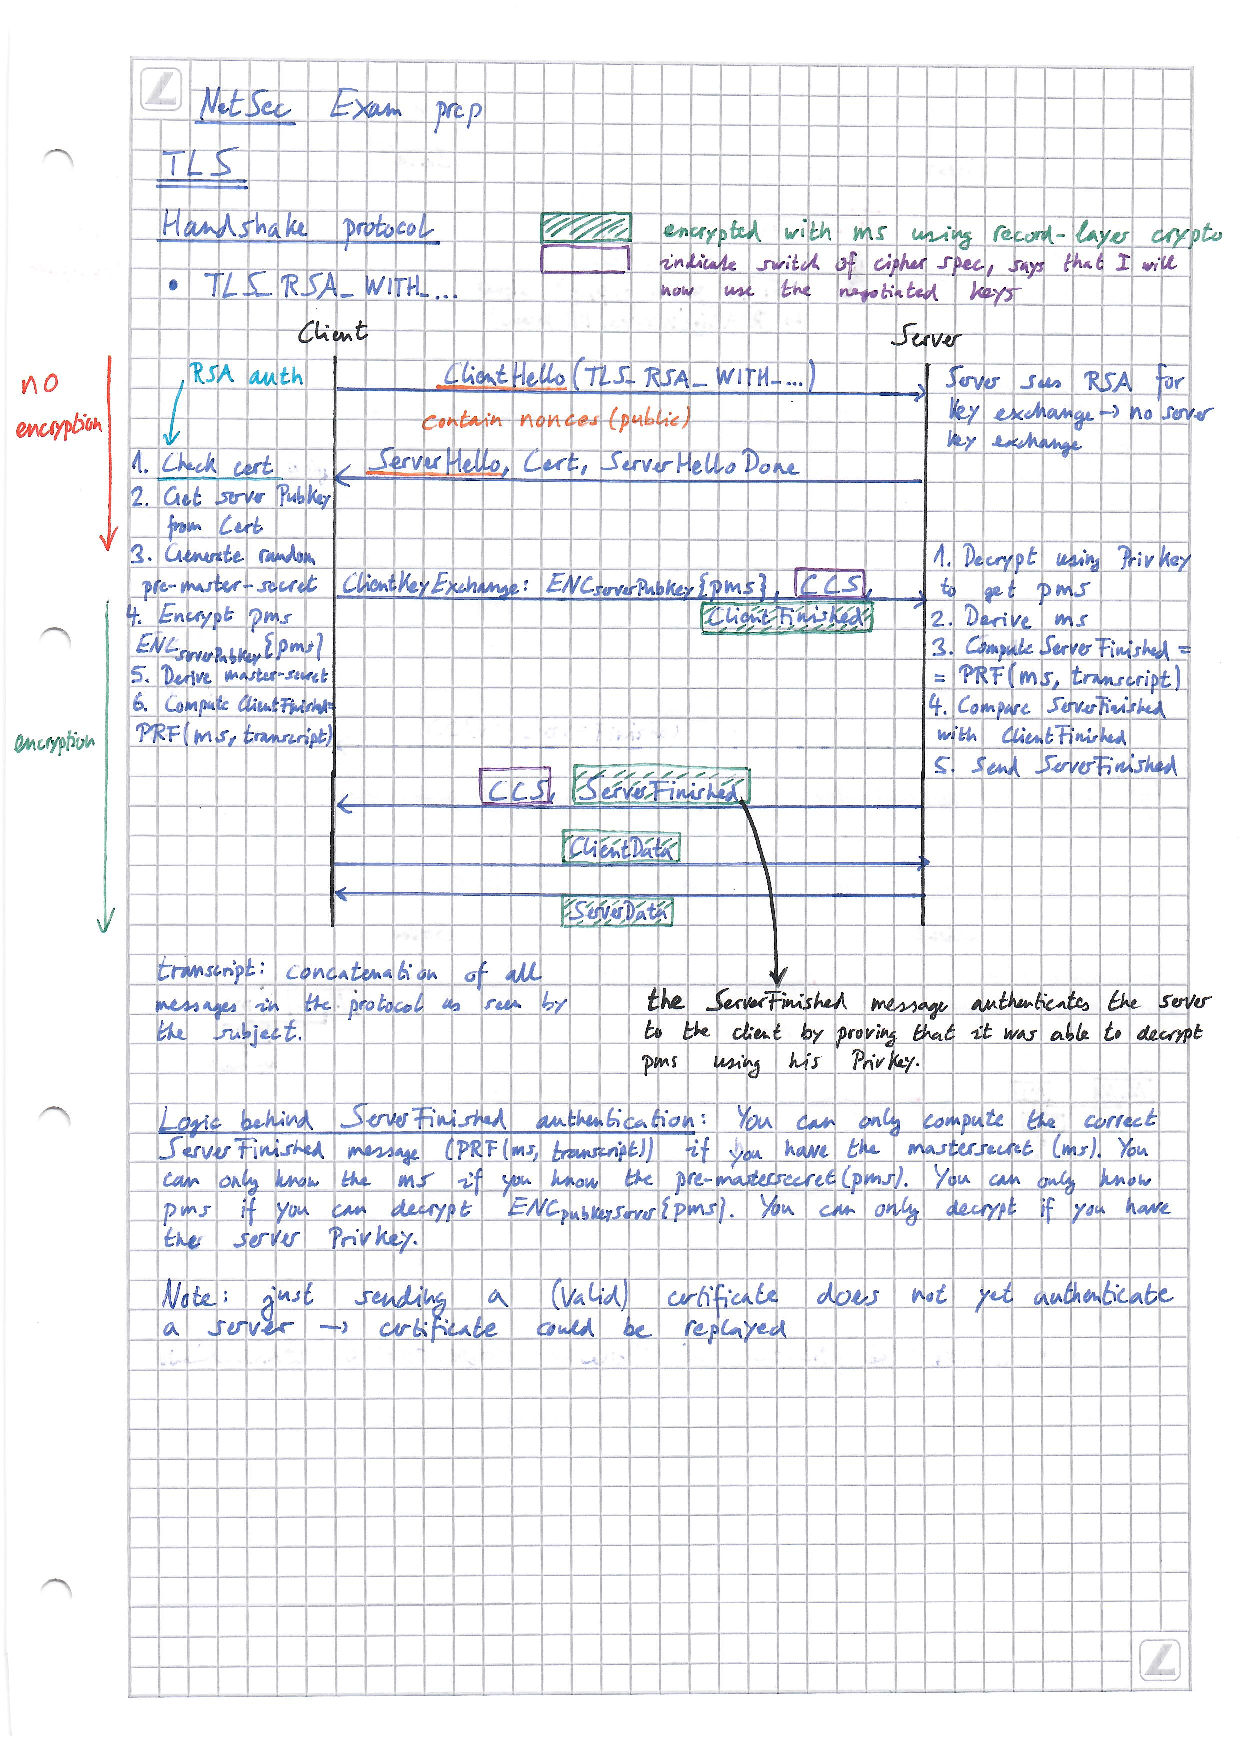
\includepdf{doc/tls_summary_1}

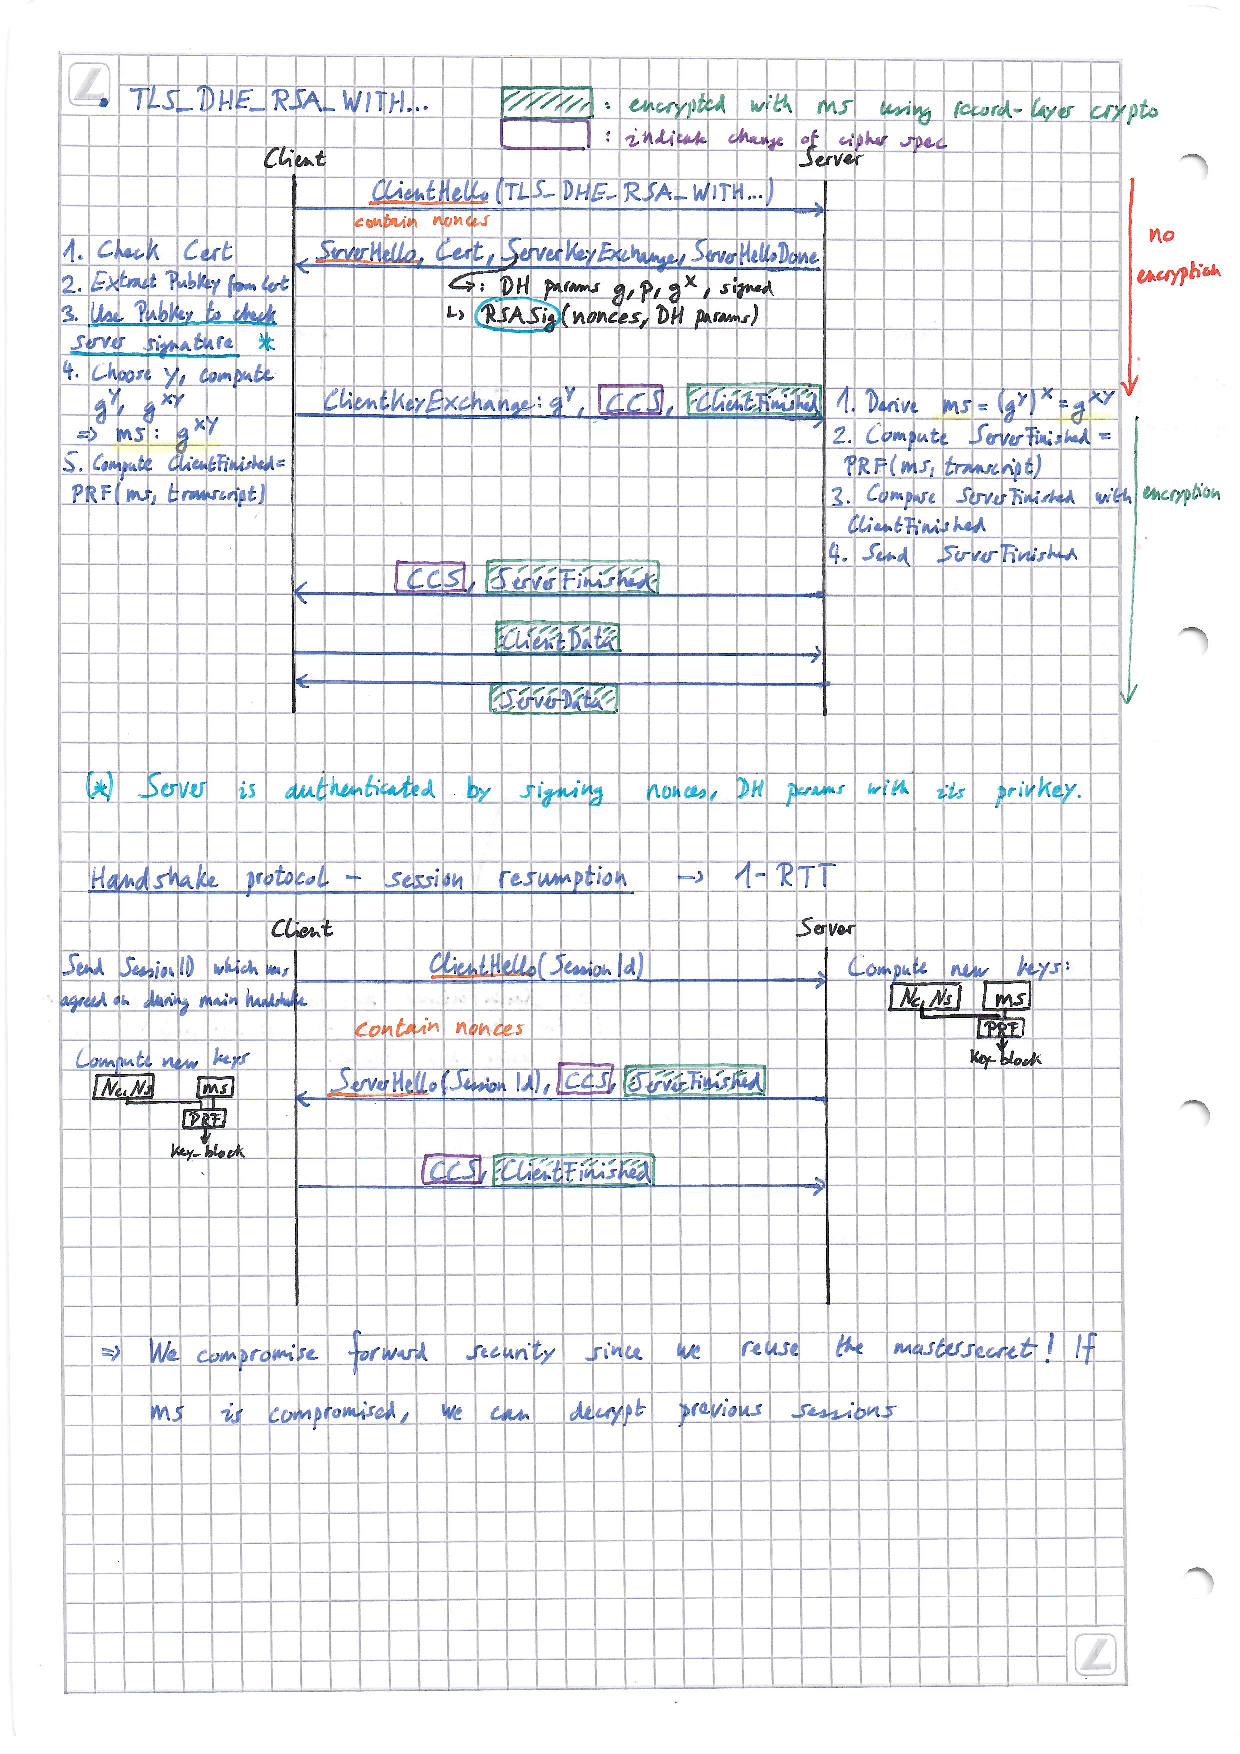
\includepdf{doc/tls_summary_2}

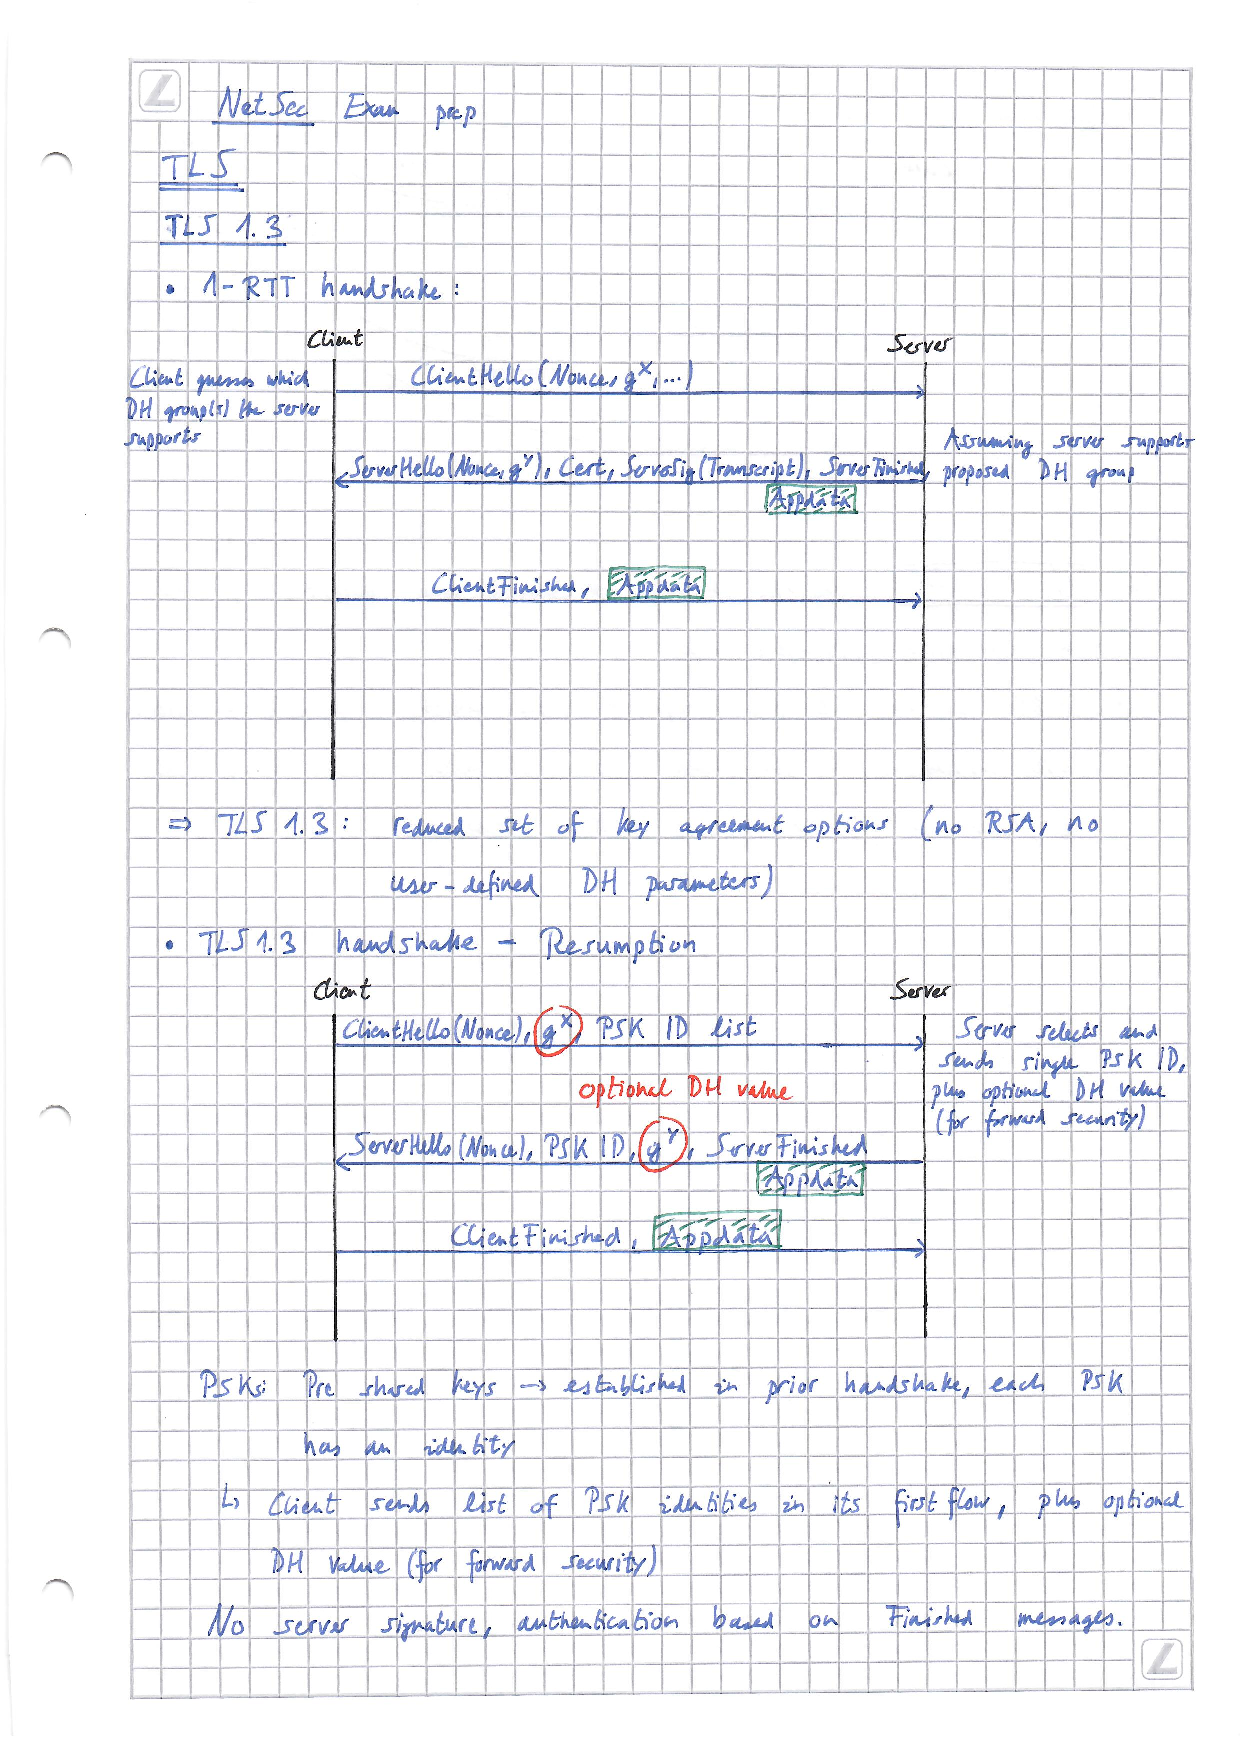
\includepdf{doc/tls_summary_3}

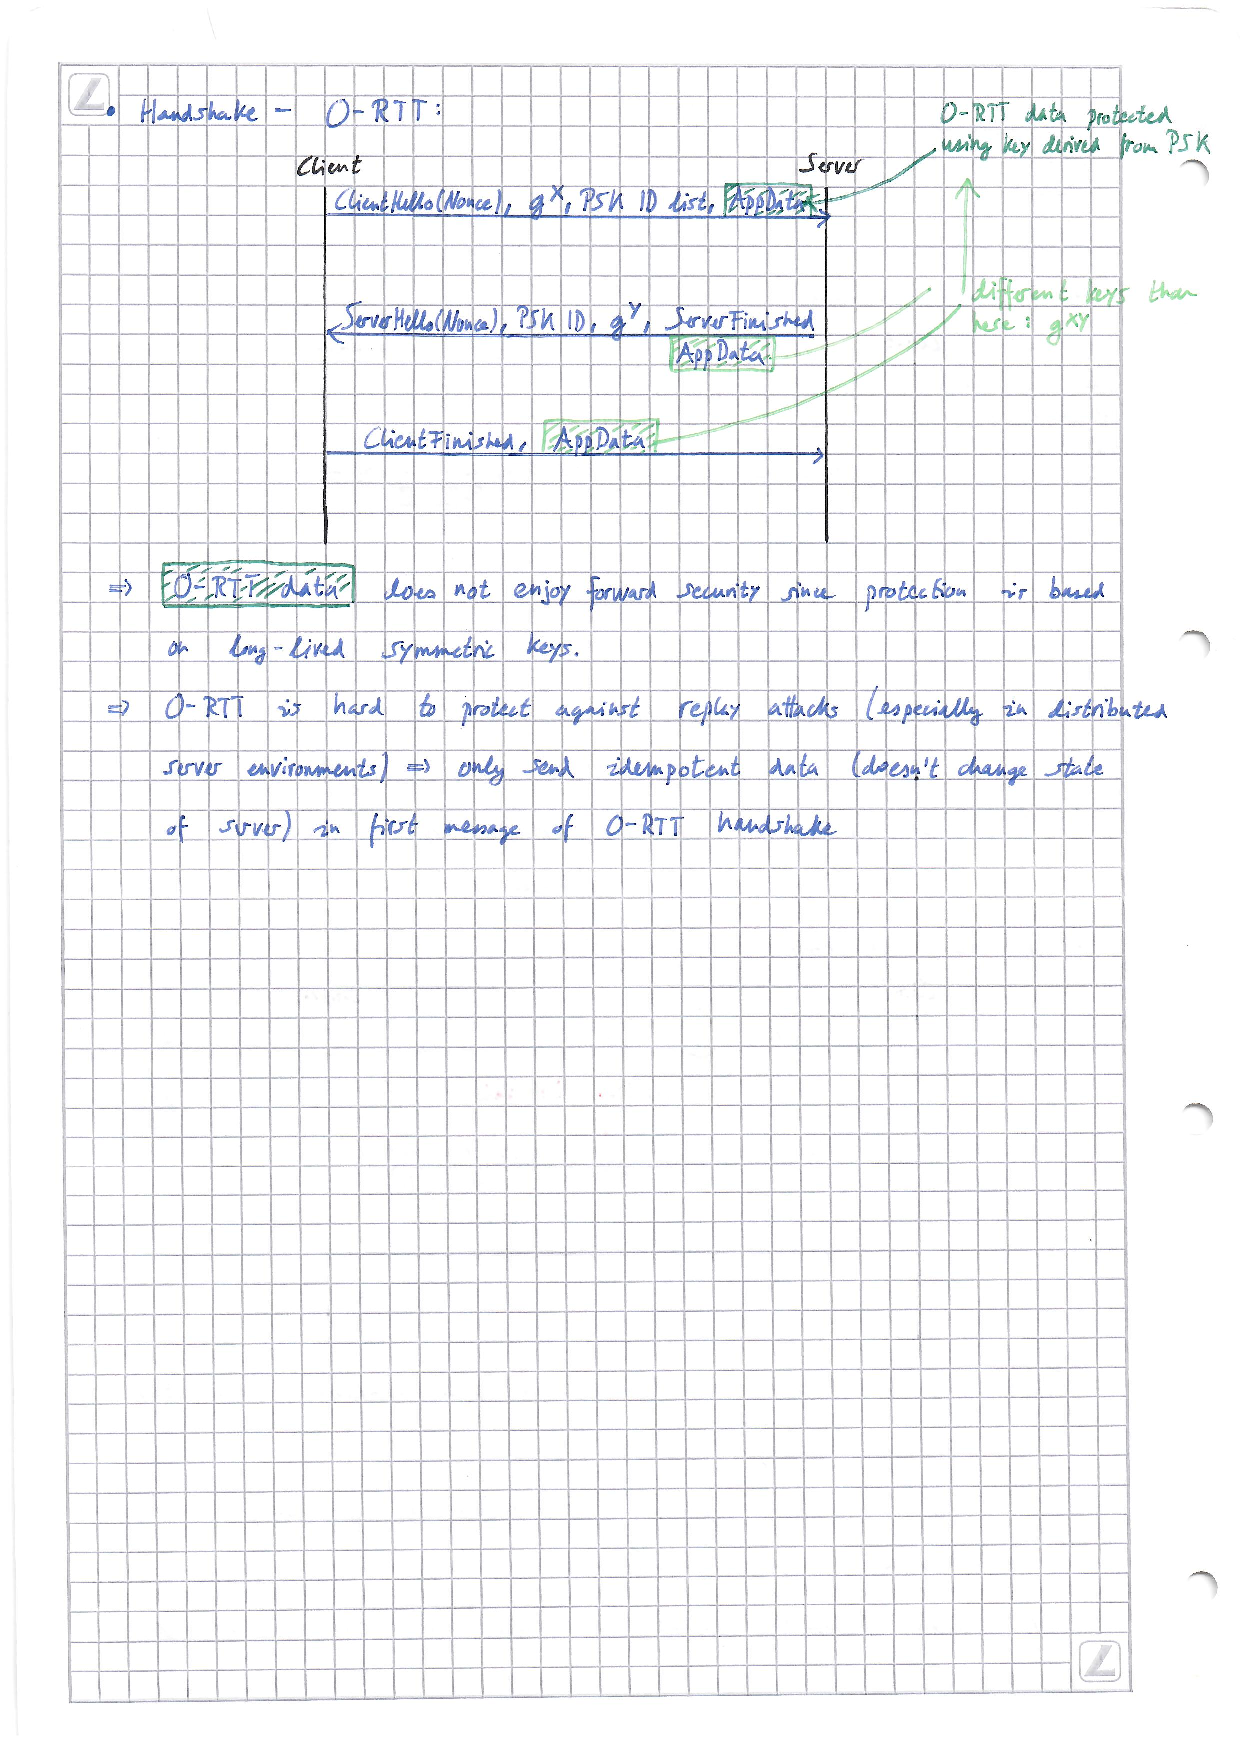
\includepdf{doc/tls_summary_4}

\section{VPNs}

A VPN creates a secure channel between two networks over an untrusted network (the Internet). VPNs and end-to-end security (TLS) complement each other. Many different VPN protocols and applications exist (IPsec, Strongswan, OpenVPN, WireGuard, ...)
Typical properties of VPN tunnels:

\vspace{-\topsep}
\begin{itemize}
	\setlength{\itemsep}{0pt}
	\setlength{\parskip}{0pt}
	\item Similar security properties as the TLS record protocol:
	\begin{itemize}
		\item Authentication of the source, integrity (MACs)
		\item Confidentiality (symmetric encryption)
		\item Replay suppression (sequence numbers)
	\end{itemize}
	\item Some tunneling protocols do not provide encryption or authentication
\end{itemize}
\vspace{-\topsep}

Typical VPN setups:

\vspace{-\topsep}
\begin{itemize}
	\setlength{\itemsep}{0pt}
	\setlength{\parskip}{0pt}
	\item secure connection between two physically separated networks (site-to-site)
	\item secure connection of a remote host to company/university network (host-to-site)
	\item VPN as a “secure” proxy (avoid tracking, spoof location, circumvent censorship)
\end{itemize}
\vspace{-\topsep}

\textbf{Why do we need VPNs when we have TLS?}

\vspace{-\topsep}
\begin{itemize}
	\setlength{\itemsep}{0pt}
	\setlength{\parskip}{0pt}
	\item If we only want to operate on layer 3 (e.g. company printer network) and still be secure
	\item When only using TLS: we still leak metadata
	\item HTTPS doesn't hide layer 3 information (srcIP, dstIP)
	\item VPNs protect all traffic ('blanket' security): DNS requests, accessing webservers without TLS
	\item VPNs can give access to services in private networks or behind firewalls
	\item VPNs allow to spoof your location
\end{itemize}
\vspace{-\topsep}

\textbf{Why do we need TLS when we have VPNs?}

\vspace{-\topsep}
\begin{itemize}
	\setlength{\itemsep}{0pt}
	\setlength{\parskip}{0pt}
	\item With VPNs, data is only secure inside the tunnel. But the data needs to somehow get to and from the tunnel. VPNs provide no security outside the tunnel
	\item VPN server can see all unencrypted traffic. TLS is still necessary.
	\item With a VPN it is not possible to authenticate a webserver, only the tunnel endpoint.
	\item VPNs need initial credential setup, TLS can be setup without knowing each other
\end{itemize}
\vspace{-\topsep}

There are many different VPN protocols but only one TLS. Why?
Because TLS is universal, everybody should be able to access webservers securely through TLS.  We thus need a globally universal standard. VPNs are setup by companies, universities, private person etc. and it only affects their clients, employees etc.. For VPNs, we can thus use whatever we want.

\subsection{IPsec}

IPsec is a very large and complicated protocol. The tunnel is setup at layer 3 (network). In IPsec, we also use sequence numbers (like in TLS) \textit{but} they are included in the packets (while TLS doesn't include sequence numbers in the packet). That's because IPsec runs on top of IP and IP is best-effort transport. The ordering of packets can thus be off at the receiver. That's why sequence numbers need to be in the packets. What if we are tunneling UDP traffic?
The numbers are also there to avoid replay attacks. Each party has a sliding window so that it can
detect if a packet is replayed by inspecting the sequence number.

\subsubsection{Internet key exchange (IKEv2)}

IKE is used to setup a security association (SA). In IKE, we have an anonymous DH exchange. This provides forward security and does not leak identities (as e.g. TLS does) since no authentication data is sent in plaintext. The disadvantage is that anonymous DH is vulnerable to an active MiTM attack.

\begin{figure}[t!]
	\centering
	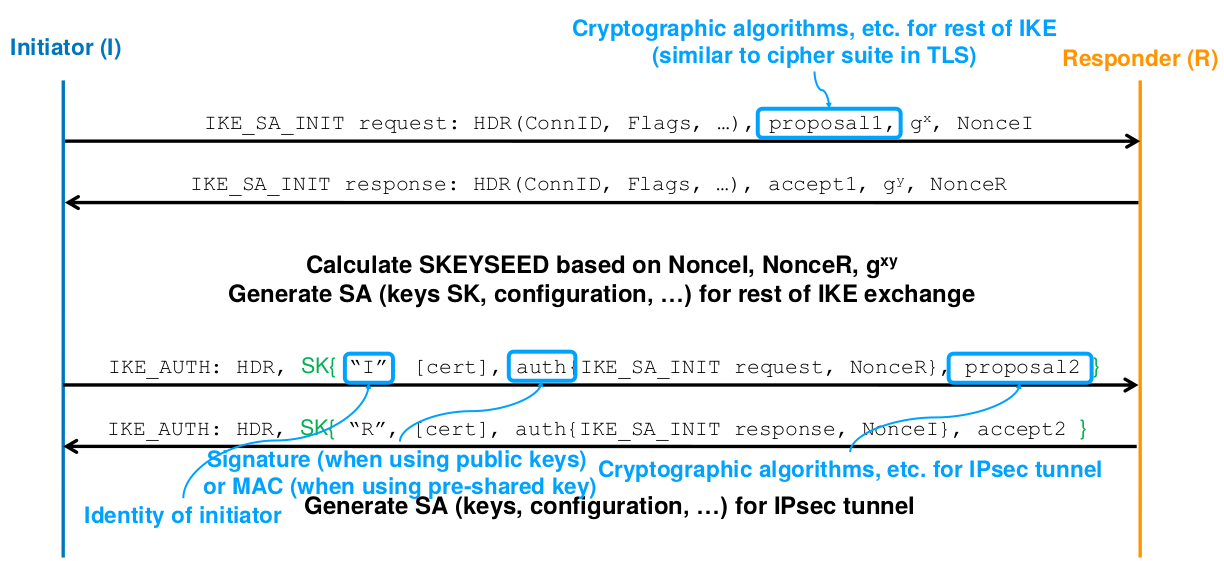
\includegraphics[width=0.9\linewidth]{figures/ikev2}
	\caption{Internet key exchange (IKEv2)}
	\label{fig:ikev2}
\end{figure}

\subsubsection{IPsec session}

After an SA was setup using IKE, we encapsulate packets and tunnel them between SA endpoints. Encapsulation works as follows:

\vspace{-\topsep}
\begin{itemize}
	\setlength{\itemsep}{0pt}
	\setlength{\parskip}{0pt}
	\item Add ESP trailer: Padding, type encapsulated (original) packet
	\item Encrypt packet and trailer
	\item Add ESP header: SA identification, sequence number
	\item Create Integrity Check Value (ICV): MAC over original packet, ESP	header, ESP trailer
	\item Add new IP header
\end{itemize}
\vspace{-\topsep}

\begin{figure}
	\centering
	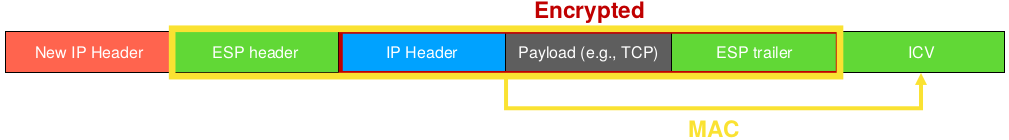
\includegraphics[width=0.7\linewidth]{figures/ipsec_encapsulation}
	\caption{IPsec encapsulation security payload (ESP) in tunneling mode}
	\label{fig:ipsecencapsulation}
\end{figure}

Similarly, decapsulation:

\vspace{-\topsep}
\begin{itemize}
	\setlength{\itemsep}{0pt}
	\setlength{\parskip}{0pt}
	\item Strip off outer IP header
	\item Look up keys and configuration using information in ESP header
	\item Check MAC
	\item Strip off authentication tag and ESP header
	\item Decrypt original packet
	\item Remove ESP trailer
	\item Forward original packet
\end{itemize}
\vspace{-\topsep}

\begin{figure}[hb]
	\centering
	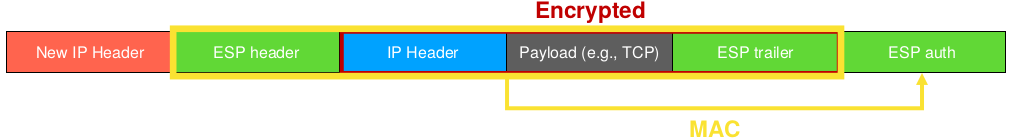
\includegraphics[width=0.7\linewidth]{figures/ipsec_decapsulation}
	\caption{IPsec decapsulation and decryption}
	\label{fig:ipsecdecapsulation}
\end{figure}

\subsection{Wireguard}

WireGuard is a modern lightweight VPN that only has roughly 4000 LOC (opposed to OpenVPN with 600'000 LOC!).\\
WireGuard relies on simple configuration and no cryptographic agility. It only uses state-of-the-art primitives: Curve25519 (signatures), ChaCha20 (encryption), Poly1305 (authentication). The small codebase provides minimal attack surface and is formally verifiable. (Even Linus Torvalds praised his love for WireGuard...)

\subsubsection{Authentication and keys}

Each peer has a static key pair. Initiator: $S_I^{pub}, S_I^{priv}$, Responder: $S_R^{pub}, S_R^{priv}$. Peers specify in configuration which public keys are authorized. WireGuard uses a 1-RTT handshake during which each peer generates an ephemeral key pair: Initiator: $E_I^{pub}, E_I^{priv}$, Responder: $E_R^{pub}, E_R^{priv}$. Symmetric keys are then derived from four DH combinations: $$\{DH(S_I,S_R), DH(S_I,E_R), DH(E_I,S_R), DH(E_I,E_R)\}$$

\begin{figure}[hb]
	\centering
	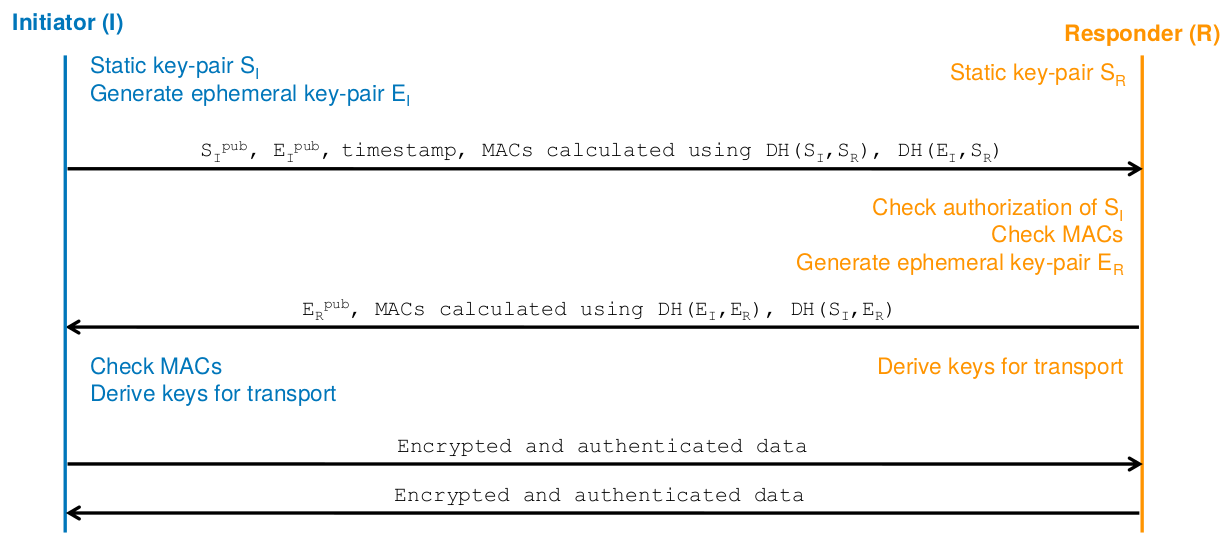
\includegraphics[width=1\linewidth]{figures/wireguard_handshake}
	\caption{WireGuard 1-RTT handshake}
	\label{fig:wireguardhandshake}
\end{figure}

The WireGuard protocol is connectionless. A series of timers, both based on message counts and time, are used to steer key renegotiation, handshakes and session termination. The strict key rotation timers \texttt{(REKEY\_AFTER\_MESSAGES, REKEY\_AFTER\_TIME)} and the ephemeral
ECDH session key exchange guarantee PFS.

\subsubsection{DoS protection}

Since VPN servers need to do expensive crypto, they are susceptible to (D)DoS attacks. A WireGuard implementation can choose to respond with a cookie instead of processing the handshake: the initiator will then use this cookie as a key for computing HMACs of their message. The cookie mechanism of IKEv2 is very similar to the one just described. However, an important difference between the two is that Wireguard requires an additional MAC on the handshake message — using the public key of the responder as HMAC key. This allows the responder to stay completely silent — not responding even with a cookie — unless the initiator knows its public key. (Remember that “public” key do not need to be publicly accessible, often they are not).

\newpage

\section{Anonymous communication systems}

Why are VPNs not enough? VPN server still sees metadata such as srcIP, dstIP, ports, metadata etc. We need something stronger for anonymous communication. 

\subsection{Terminology: “anonymity”}

\vspace{-\topsep}
\begin{itemize}
	\setlength{\itemsep}{0pt}
	\setlength{\parskip}{0pt}
	\item Sender anonymity: adversary knows receiver, may learn message, sender is unknown. The sender anonymity set is the set of all possible senders, which can be used as a (rough) metric. A small set means little anonymity.
	\item Receiver anonymity: Adversary knows sender, may learn message, receiver is unknown. The sender needs a return address: the receiver provides a token (since the sender doesn't know the receiver) and the token will be used to direct the message. Receiver anonymity set is the set of all possible receivers.
	\item (Sender-receiver) unlinkability: Adversary knows senders, knows receivers, link between senders and	receivers is unknown. Multiple users need to communicate at the same time.
	\item Unobservability: Adversary cannot tell whether any communication is taking place.
\end{itemize}
\vspace{-\topsep}

The following holds: $Unobservability \rightarrow Anonymity \rightarrow Unlinkability$

\subsection{How to send a message anonymously}

\subsubsection{Broadcast}

Receiver anonymity is guaranteed, sender can be de-anonymized (localization through triangulation)!. Alternative: hijacked connection (burner phone, hacked WiFi, network ID ≠ personal sender ID).

\subsubsection{Mixnets}

Simple idea: use a proxy or VPN. The proxy has to be trusted $\rightarrow$ to avoid fully trusting the proxy: Layered encryption. However, the adversary may be able to link inputs
and outputs (timing)!\\\
The proxy should perform \textbf{batching and mixing}. Batching: collect a number of messages
before forwarding (threshold). Mixing: change the order of (mix) the messages.\\
An adversary can still mount an intersection attack: Often, users only communicate with a
small subset of other users. Idea: every time a message is seen by the target, register the sets of destinations. To achieve full unobservability, use \textbf{cover traffic}, both for sending and receiving. Now we are fully anonymous... as long as the mix is trusted!. We should use multiple mixes to avoid single point of failure (cascade). Each mix should only know its direct neighbor and only the first mix should know the sender and only the last mix should know the receiver.\\
How do we handle return addresses? Alice prepares a return address and encloses it in her first message. That address contains layered information.

\subsection{Circuit-based systems (AKA onion-routing system)}

Mix-nets are very secure but very slow. We want a system that can support web browsing. Main ideas: use layered encryption, no batching and mixing, no cover traffic. Flow-based: establish a virtual circuit (keys) once per flow, reuse it for all packets in the flow using only symmetric key crypto. The threat model is constrained: only a local adversary (e.g. ISP) which cannot launch confirmation attacks.\\
\textbf{Terminology:} Circuit-based anonymous communication systems, commonly known as Onion Routing Systems. The nodes are called relays (also nodes or routers). The virtual circuit is also called tunnel.

\subsubsection{Circuit setup}

The sender negotiates shared keys with all relays on the path (this requires expensive asymmetric key cryptography).\\
\textbf{Direct circuit setup:} a packet is sent through the whole system and returned and at each step the state is generated. The encryption keys of data are only based on public keys of relays. Thus (immediate) FS does not hold since no ephemeral information is used.\\
\textbf{Telescopic circuit setup:} Keys are negotiated one relay at a time. The circuit is “extended” by one hop at a time (that’s why it is called telescopic). Ephemeral session keys are negotiated before the circuit is extended. This setup is slower... but it offers immediate forward secrecy: As soon as the circuit is closed, the session keys are deleted.

\subsubsection{Data forwarding}

The sender has established a circuit (keys and per-link IDs). A data packet is encrypted as usual (layered encryption). The ID of the next relay is added in clear text. To protect against network adversaries, links can be encrypted (TLS).

\subsubsection{Circuit tear-down}

Can be initiated both by sender and by intermediate relays. The sender communicates the tear-down to one relay at a time, starting from the furthest away. The exit relay may tear down the circuit if a corrupt packet is detected, or some other attack. Circuits have a limited lifetime, so they will eventually be destroyed.

\subsection{Attacks on circuit-based anonymous-communication systems}

Many attacks have been proposed, however for many it is unclear if they fit the standard threat model. Some of them are practical, requiring limited resources. Others are only achievable by state-level adversaries (Five Eyes).

\subsubsection{Fingerprinting}

One general attack is fingerprinting. This can be done in multiple ways:

\vspace{-\topsep}
\begin{itemize}
	\setlength{\itemsep}{0pt}
	\setlength{\parskip}{0pt}
	\item Passive traffic analysis: The adversary observes the edges of the network, recording traffic patterns.
	\item Active traffic analysis: 
	\begin{itemize}
		\item The adversary actively modifies packet timings: Inter-packet timings (delaying/reordering packets), packet drops also possible but detectable
		\item Flow watermarking: inject one bit of information (marked or not)
		\item Flow fingerprinting: inject multiple bits (e.g., sender IP address!)
	\end{itemize}
	\item Website fingerprinting: Many websites have a distinct pattern of traffic they receive and send. Adversary can keep a database of patterns and compare traffic recorded from a single observation point (ISP, WiFi users,...)
\end{itemize}
\vspace{-\topsep}

There are two possible approaches on how to defend against fingerprinting:

\vspace{-\topsep}
\begin{itemize}
	\setlength{\itemsep}{0pt}
	\setlength{\parskip}{0pt}
	\item Randomization: make the fingerprint look random, each user always has a new, random fingerprint.
	\item Uniformity: make all the fingerprints look the same, all the users share a common	fingerprint. This is what the TOR browser tries to enforce. All Tor Browser user supposedly share the same fingerprint, increasing their anonymity set. Numerous patches are used to limit plugins, ask permission for HTML Canvas, restrict WebSockets, reduce available fonts, standardize the User-Agent header, and limit many other fingerprinting techniques. Even window size is considered sensitive: the browser will warn you if you attempt to maximize its window (you would leak the size of your monitor).
\end{itemize}
\vspace{-\topsep}

In order to prevent fingerprinting, you should omit \textit{everything} that makes you stand out: don't install any plugins, never use TOR in fullscreen mode (gives away your screen resolution), don't type inside the browser, type inside a text-editor and copy-paste messages into webforms, etc.

\subsubsection{Higher-layer attacks}

\vspace{-\topsep}
\begin{itemize}
	\setlength{\itemsep}{0pt}
	\setlength{\parskip}{0pt}
	\item OS Network stack fingerprinting (OS, browser, window size, user-agent, browser plugins, etc.)
	\item Most deanonymization is still done through other means: Trick user into downloading malware, trick user into downloading file that will access the Internet directly, analyze user behavior like texts.
\end{itemize}
\vspace{-\topsep}

To achieve anonymity, all layers need to be anonymized: Any gap will break anonymity!

\subsection{TOR}

TOR basics:

\vspace{-\topsep}
\begin{itemize}
	\setlength{\itemsep}{0pt}
	\setlength{\parskip}{0pt}
	\item Circuits established over 3 relays
	\item Telescopic setup (forward secrecy!)
	\item Per-hop TCP, established on the fly to avoid TCP stack fingerprinting
	\item Per-hop TLS (except on the last hop). Multiple circuits over same TLS connection. End-to-end HTTPS is possible.
	\item Main tool: Tor browser (Firefox)
\end{itemize}
\vspace{-\topsep}

TOR additional features:

\vspace{-\topsep}
\begin{itemize}
	\setlength{\itemsep}{0pt}
	\setlength{\parskip}{0pt}
	\item Exit policies (exit can restrict the destinations	they connect to)
	\item Multiple streams per circuit (helps with performance, weakens anonymity)
	\item Censorship resistance (bridges)
	\item Hidden services: Provide receiver anonymity, use .onion URL (not in DNS). The name is the hash of the HS’s public key.
\end{itemize}
\vspace{-\topsep}

\subsubsection{Cells}

If a relay obtains a cell: it looks up keying material from circuit id and will decrypt the payload which contains sets of fields. The relay then checks the digest and if it matches it looks at the cmd.

\begin{figure}[hb]
	\centering
	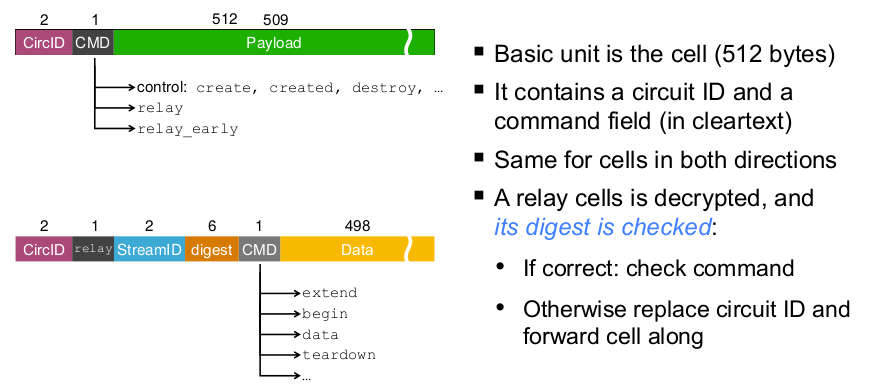
\includegraphics[width=0.7\linewidth]{figures/tor_cell}
	\caption{TOR cell}
	\label{fig:torcell}
\end{figure}

\subsubsection{Directory authorities}

How do the clients know what relays there are? 10 directory authorities (servers) running a consensus algorithm. The authorities track the state of relays, store their public keys. Client software (Tor browser) comes with a list of the authorities’ keys (If an adversary can supply the list, de-anonymization is trivial!). A client accepts a consensus document if signed by ≥ 50\%. The centralized authorities are an important weakness of Tor. An adversary compromising 5 authorities can compromise Tor. Every relay periodically reports a signed statement (state, stats.) DAs also act as bandwidth authorities: verify bandwidth of nodes.\\
Sybil protection: DAs limit the number of relays per IP subnet.

\subsubsection{Censorship resistance in Tor}

The Tor network contains a number of bridge relays (or bridges). Not (all) publicly listed, instead distributed through friends networks. This is used to circumvent censors which black-list Tor relays. Problem: deep packet inspection allows detection of Tor traffic
Solution: obfuscate the traffic (pluggable transports)

\subsubsection{Circuit setup}

Who is authenticated on the first hop? Alice is \textit{not}. The entry guard is since Alice encrypted her ephemeral DH value $g^{x_1}$ with the entry guard's pubKey. The entry guard then sends back $g^{y_1}$ and a hash of $g^{x_1y_1}$ which it can only do if it was able to decrypt $g^{x_1}$ which it can only do if it has the privKey.
\begin{figure}[hb]
	\centering
	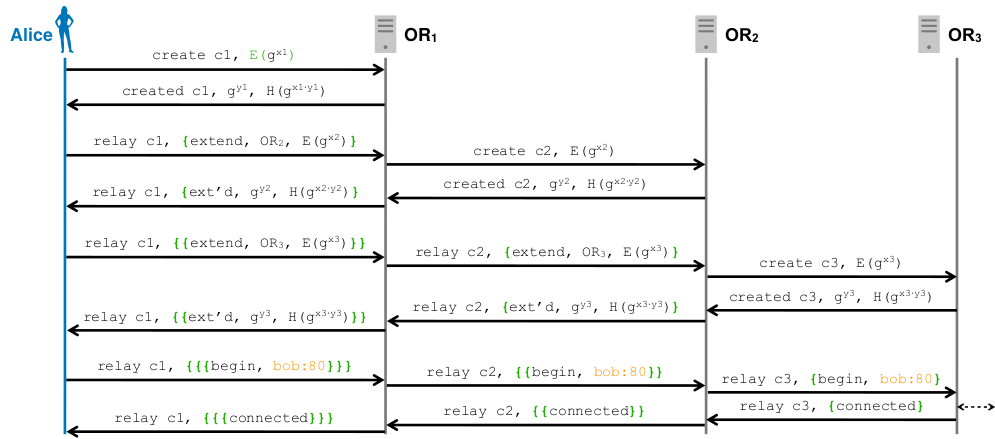
\includegraphics[width=0.9\linewidth]{figures/tor_circuit_setup}
	\caption{Circuit setup with three hops}
	\label{fig:torcircuitsetup}
\end{figure}

\section{DNS Security}

The Internet is a critical infrastructure, yet its operation depends on the fundamentally insecure DNS. DNS provides a mapping of names to resources of several types. However, DNS, as a robust key protocol of the Internet, is also a formidable attack vector for cyber criminals:

\vspace{-\topsep}
\begin{itemize}
	\setlength{\itemsep}{0pt}
	\setlength{\parskip}{0pt}
	\item DNS helps cybercriminals to setup services that are hard to hunt-down or shut-
	down (Botnets, Fast- \& Domain Flux)
	\item DNS helps building hidden channels (tunneling)
	\item is abused for powerful denial of service attacks
	\item is abused for various impersonation attacks
\end{itemize}
\vspace{-\topsep}

\subsection{Domain Name System (DNS)}

DNS uses hierarchical namespaces to scale: tree structure down from root level ".", to top-level domains (TLD, e.g. .com) to second-level domains (SLD, e.g. google.com). A fully qualified domain name (FQDN) for example is mail.ethz.ch. The hierarchy descends from right to left. Domains are namespaces: everything below .com is the \textit{com} domain, everything below .ibm.com. is the \textit{ibm.com} domain.

\begin{figure}[hb]
	\centering
	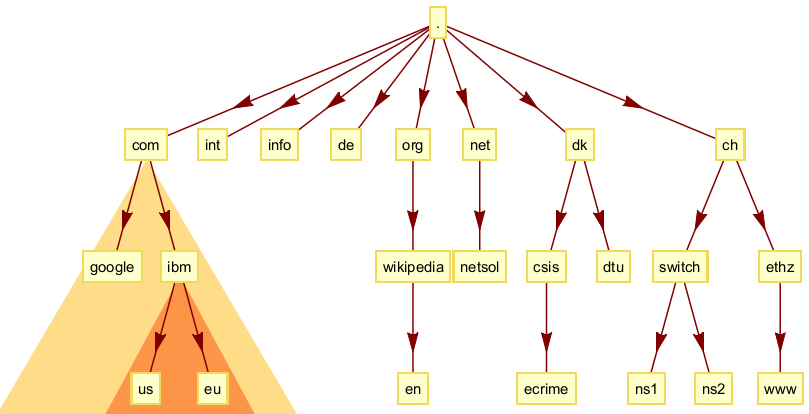
\includegraphics[width=0.6\linewidth]{figures/dns_namespace_hierarchy}
	\caption{DNS Namespace Hierarchy}
	\label{fig:dnsnamespacehierarchy}
\end{figure}

\textbf{DNS protocols \& elements}

\vspace{-\topsep}
\begin{itemize}
	\setlength{\itemsep}{0pt}
	\setlength{\parskip}{0pt}
	\item Protocol: simple client-server protocol, operating on TCP/UDP port 53. No encryption, authentication nor integrity built into original protocol.
	\item Name server: Servers that map names to objects (= resource records RR). Authoritative: server is authoritative for a specific zone. Caching/Resolver: server resolves domains recursively, caches	results.
	\item Resolver: Client side of DNS resolution, responsible for initiating and sequencing the queries that ultimately lead to a full resolution. Stub resolver: piece of software running on a client that sends recursive DNS requests to a recursive resolver. Recursive resolver: processes DNS resolution iteratively to	provide full answer: it contacts all the different servers at the different domain levels to get the final answer.
\end{itemize}
\vspace{-\topsep}

Each DNS response has a TTL. Caching resolvers will redo a recursive lookup once the TTL for a cached response has expired. A shorter TTL leads to shorter living cache entries, leading to faster refreshes for end users in case of an update. However, this means that there will be more load on the DNS servers for doing the recursive lookup again.

\subsubsection{Root servers}

DNS root name servers are the key to the Internet kingdom: the DNS root zone is served by 13 root server clusters which are authoritative for queries for the top level domains. Every name resolution in the Internet either starts with a query to a root server, or, uses information that was once obtained from a root server. DNS root name servers have the official names a.root-servers.net to m.root-servers.net. They only resolve the IP addresses for the top-level name servers (TLD).

\subsubsection{Top-Level name servers}

A domain name registrar is an organization that manages the reservation of second-level Internet domain names (SLD) below a given top-level domain (TLD). A domain name registrar must be accredited by a top-level domain registry and/or a country code top-level domain (ccTLD) registry. Based on the domain registration database, the top-level name server points resolvers to the authoritative name server of the SLD.

\subsubsection{Authoritative Domain Server}

The authoritative name server for a second-level domain is managed by private entities or on behalf of private entities that have registered a domain name. The authoritative name server has all records for a zone configured and can provide the final / authoritative information.

\subsubsection{Name Server Roles}

\begin{figure}[hb]
	\centering
	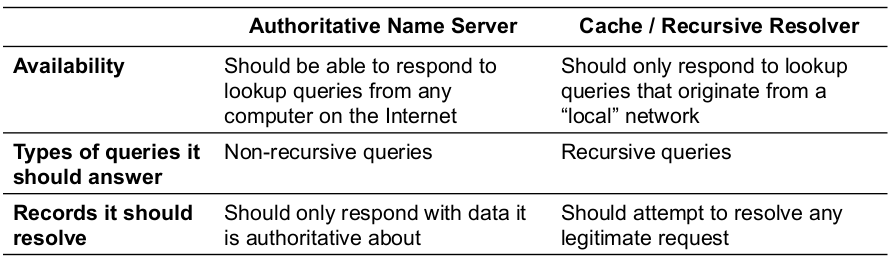
\includegraphics[width=0.7\linewidth]{figures/dns_name_server_roles}
	\caption{DNS - Name Server Roles}
	\label{fig:dnsnameserverroles}
\end{figure}

\subsection{DNS spoofing}

\textbf{Attack Methodology:} Insertion of incorrect resolution information by a host that has no authority to provide that information. DNS requests rely on UDP. Each request is assigned a unique identifier (TXID) to help manage multiple requests. DNS server responds, including the same TXID, client ignores responses with different TXIDs.\\
\textbf{Example:} Client requests www.bank.com. If the attacker is on the same network, she can sniff traffic and look for specific DNS requests. As soon as shes sees the request, she can immediately send back a DNS reply for www.bank.com however with a spoofed IP that points to some location she owns. General rule: first reply wins! When to legitimate reply arrives a bit later, it is ignored. Most likely, the attacker is faster: physically closer, she can drop packets, recursive resolution takes a lot of time, attacker could overload resolver. The TXID can be sniffed or guessed.

\subsection{Distributed Reflection / Amplification DDoS}
\label{dns_ddos}

\textbf{Attack Methodology:} DNS queries are typically transmitted over UDP - they are fire and forget. The source IP can be spoofed and the receiver has no way of determining its veracity before responding. The attacker will spoof the srcIP to the victim's IP - the response will thus be reflected to the victim and overload his servers. DNS also is capable of generating a much larger response than query (e.g. \texttt{dig ANY isc.org @x.x.x.x} query is 64 bytes, the response is 3,223 bytes). There are many powerful and well connected DNS servers, which can be abused to redirect large DNS responses to any target. The key to this attack are \textit{open} DNS resolvers (recursive resolver that replies to any DNS query, coming from any device
on the Internet).\\
\textbf{Key ingredients of a reflection/amplification attack:} stateless protocol (UDP), can spoof the srcAdr (reflection), small request generates large response (amplification). Other protocols that also fulfill these criteria: memcached, NTP.\\
\textbf{Mitigation:} Source IP verification (reject packets with source addresses not reachable via the actual packet’s path), disable recursion on authoritative name servers, limit recursion to authorized clients, Response Rate Limiting (RRL).\\
However, the main mitigation is hosting a service on different locations in the internet, s.t. it gets harder for an attacker to target all possible locations. Using BGP anycast, the same IP address is advertised on different locations on the internet.\\
A user is directed to the nearest service location. This helps to distribute the load on different sites. There are CDN services like Akamai or CloudFlare that offer this as a service.

\begin{figure}[hb]
	\centering
	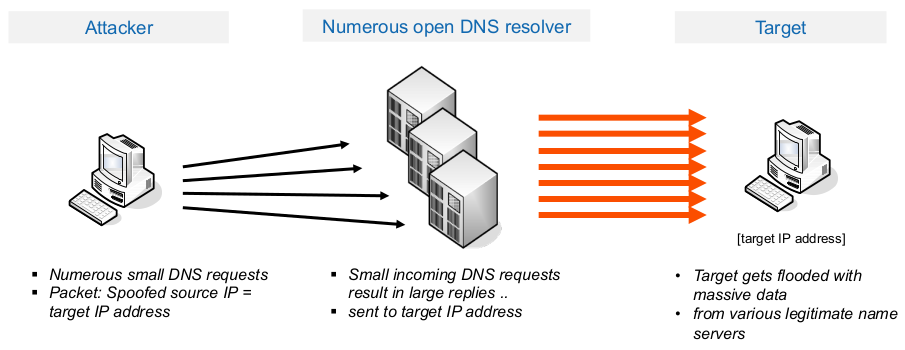
\includegraphics[width=0.7\linewidth]{figures/dns_reflection_amplification_ddos}
	\caption{Distributed Reflection / Amplification DDoS}
	\label{fig:dnsreflectionamplificationddos}
\end{figure}

On TCP, this attack would not work as is since the second message after the TCP SYN is not the DNS response but the TCP SYN ACK. The TCP ACK would go to the victim (due to the srcIP spoofing). The DNS response would be the second message sent by the server. However, the attacker could reply with the third handshake message + payload after inter-epting the replies and dropping them. If the attacker is not Dolev-Yao, which is often the case, the attack would become tricky to perform.

\subsection{DNS Cache Poisoning}

\textbf{Attack Methodology:} Attacker abuses caching capability of domain name system. Inject faked Domain\textgreater IP information into cache of caching name server. Subsequent requests by any user to this server are served this fake information from cache.\\
\textbf{Example:} Attacker owns authoritative name server for bad.com and tricks user to resolve bad.com (phishing, hacked site, attachment, hidden picture, ..). Attacker adds multiple resolution entries for e.g. bank.com into the \texttt{ADDITIONAL SECTION} of the DNS reply  for bad.com. The client will cache this information even though he didn't ask for it.\\
\textbf{Mitigation:} The example attack is no longer really a problem since software no longer accepts entries from additional section which are for different domains.

\subsection{DNS/Domain Hijacking}

\textbf{Attack Methodology:} Domains are registered with a domain registrar. The DNS information is as secure as the Web App, backend processes, or the passwords of the registrar and the domain owner. An attacker could for example hack the web app of the domain registrar (e.g. godaddy, namecheap, etc.), brute-force user passwords (or get it from data breach) and then manipulate the domain registration entries directly at the registrar (change name servers, and password of registrars Web App).\\
\textit{Your DNS security is as good as the security of the domain registrar, and your credentials.}

\subsection{Local Host / Network LAN \& WAN}

\textbf{Attack Methodology:} Manipulate DNS settings on local host, or provisioning of DNS settings in local network. Have target point to attackers name server.Various attack vectors:

\vspace{-\topsep}
\begin{itemize}
	\setlength{\itemsep}{0pt}
	\setlength{\parskip}{0pt}
	\item Network attack:
	\begin{itemize}
		\item WAN: Attack poorly protected client router of Internet Service Providers (ISP)
		\item LAN: Attack the DHCP exchange in local network. DHCP has no authentication and includes the default name server -\textgreater spoof it. Again, the attacker will be able to outpace the DHCP response of the DHCP server.
	\end{itemize}
	\item Host Attack: Upon compromise of target, manipulate local hosts file (e.g. \texttt{/etc/hosts} for linux) (e.g. after infection). The attacker could for example add a static mapping for www.bank.com to an IP she owns. Malware often adds static mapping to hosts file for antivirus domains (e.g. map to loopback). This way, signatures are not updated.
	\item DNS Changer Botnet: Botnet changes DNS settings on infected hosts. Name server configuration now points to name server of attacker. Possible exploits are ad manipulation (Google ads), phishing (credit cards, online banking) or selling software (fake iTunes shops).
\end{itemize}
\vspace{-\topsep}

\subsection{Botnet Control - Controlling compromised machines}

Cyber criminals organize compromised machines and devices in centrally controlled botnets, consisting of thousands or millions of agents/bots. Bots are used to send spam, DDoS attacks, banking and click-fraud, bitcoin mining, etc. Criminals want to control their botnets and protect their infrastructure from take-down attempts and competitors.\\
\textbf{Botnet management requirements (criminals view):}

\vspace{-\topsep}
\begin{itemize}
	\setlength{\itemsep}{0pt}
	\setlength{\parskip}{0pt}
	\item Bot must receive new instructions and malicious capabilities ..
	\item Robustly manage 10,000+ globally distributed bots ..
	\item Botnet shall be resistant to hijack and shut-down attempts ..
\end{itemize}
\vspace{-\topsep}

\begin{figure}[hb]
	\centering
	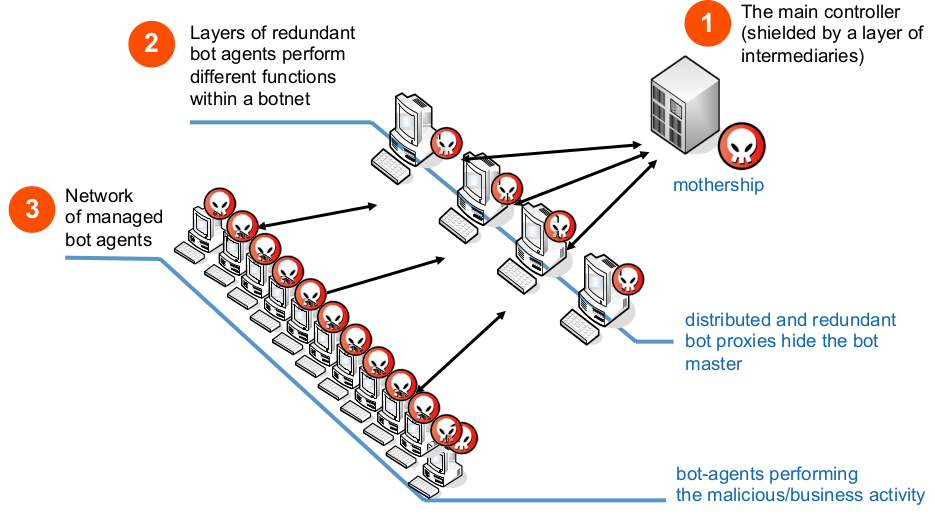
\includegraphics[width=0.7\linewidth]{figures/dns_botnet_architecture}
	\caption{DNS Botnet architecture}
	\label{fig:dnsbotnetarchitecture}
\end{figure}

The ability of a bot agent to locate the command and control (CnC) infrastructure
is a critical requirement for maintaining control of the entire botnet. However, criminals want to evade law enforcement. By using \textit{fixed IPs} it would be easy to identify bot agent and controller and blocking the botnet would be easy (one firewall rule). By using \textit{fixed domains} it would be easy to identify bot agent, harder to identify controller. Shutting down the botnet would also be harder (DNS caches). More flexibility is obtained through IP flux or domain flux: domain names and/or IP addresses change frequently both technologies are extensively used by professional botnet operators very dynamic, moving target, hard to shut down botnet.

\subsubsection{Fluxing Approaches}

A CnC resource with a given domain name (FQDN) is mapped to a new set of IP addresses as often as every few minutes: a bot agent connecting to the same FQDN actually connects to a different CnC server every 3 minutes this rapid changing aspect is commonly referred to as “Fast-Flux” the IP of unresponsive CnC nodes are taken out of flux and availability is always maintained (Quality of Service).

\vspace{-\topsep}
\begin{itemize}
	\setlength{\itemsep}{0pt}
	\setlength{\parskip}{0pt}
	\item \textbf{IP Flux:} frequent change of IP address information related to a particular fully-qualified domain name (FQDN). Example: cnc.net \textgreater multiple changing IP addresses.
	\item \textbf{Domain Flux:} frequent change and allocation of multiple fully-qualified domain names (FQDN). Example: cnc.net, cnc.ru, abc.com, xyz.ch \textgreater multiple changing IP addresses. Each bot uses a domain generation algorithm (DGA) to periodically compute a list
	of new domain names. From a practical standpoint, domain flux generates a list of “rendez-vous” points that may be used by the bot masters to control their bots.
\end{itemize}
\vspace{-\topsep}

\subsection{DNS over HTTPS (DoH)}

DOH would solve some attacks on DNS such as DNS spoofing, mass-logging of DNS requests, DNS amplification/reflection, cache poisoning, etc. However, there are disadvantages. With DOH, local caches are no longer possible – each query needs to reach the remote DoH resolver. In the case of large providers, load and latency are not a problem: anycast is used to respond to the queries in a geographically distributed way. However, this concentrates even more power in the hands of a few companies (Google, Cloudflare, etc.); the internet gets even more centralized.

\subsection{Domain Name System Security Extensions (DNSSEC)}

DNSSEC attempts to add security, while maintaining backward compatibility to the
existing DNS. DNSSEC is a set of extensions to DNS to provide resolvers: origin authentication of DNS data, authenticated denial of existence, integrity. But not availability or confidentiality.\\
DNSSEC zone data is digitally signed using a private key for that zone. A DNS server receiving DNSSEC signed zone data can verify the origin and integrity of the data by checking the signature using the public key for that zone.\\
\textbf{Process:} (1) Each DNS zone signs its data using a private key (recommended to do offline). (2) A query for a particular record returns: The requested resource record set, a signature (SIG) of the requested resource record set. (3) The resolver authenticates response using public key.

\begin{figure}[hb]
	\centering
	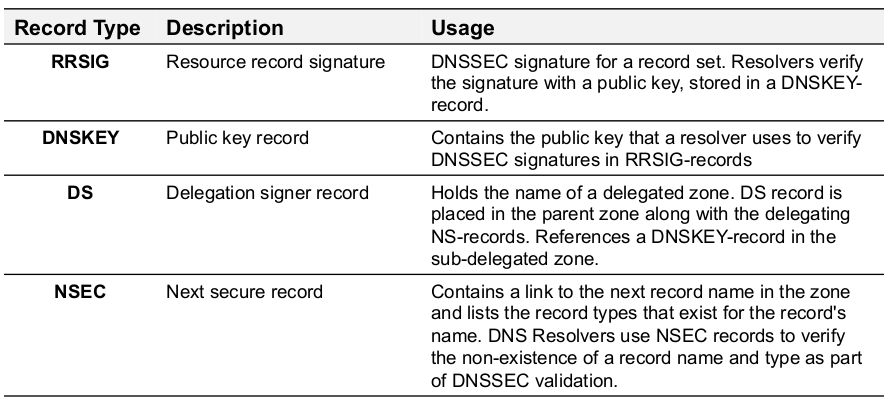
\includegraphics[width=0.8\linewidth]{figures/dnssec_resource_records}
	\caption{DNSSEC Resource Records}
	\label{fig:dnssecresourcerecords}
\end{figure}

\textbf{DS record:} The DS record contains a hash of the KSK (key signing key) belonging to the
child zone. Once the DNS resolver knows the contents of DS, it can retrieve the KSK and ZSK (zone
signing key) belonging to the child zone. KSK is checked against DS. ZSK is validated using
the KSK. Finally, if the child zone is the actual target of the query, the answer
can be checked by using the ZSK.

\newpage

\section{Firewalls, IDS \& Detection \& Evasion}

\subsection{Firewalls}

A firewall is a system used to protect or separate a trusted network from an untrusted network, while allowing authorized communications to pass from one side to the other.

\vspace{-\topsep}
\begin{itemize}
	\setlength{\itemsep}{0pt}
	\setlength{\parskip}{0pt}
	\item \textbf{Network Firewall:} Network firewalls are a software appliance running on specific hardware or as virtual instance that filter traffic between two or more networks.
	\item \textbf{Host Firewall:} Host-based firewalls provide a layer of software on one host that controls network traffic in and out of	that single machine.
\end{itemize}
\vspace{-\topsep}

Host based firewalls have context, know exactly what is running on a host. This allows for more fine-grained decisions. Host based firewalls are good for mobile devices (e.g. phones). Network firewalls are good if you e.g. can't install a firewall on a device (e.g. printer).\\

\vspace{-\topsep}
\begin{itemize}
	\setlength{\itemsep}{0pt}
	\setlength{\parskip}{0pt}
	\item \textbf{Stateless Firewall:} look at each packet on the network layer individually, no state maintained. Decisions based on packet header information. This is fast, scalable and simple but very limited.
	\item \textbf{Stateful Firewall:} keep also track of the state of the network connections, decision also based on session state. This is more powerful but: state explosion, inconsistencies, state for UDP.. The problem with state explosion: an attacker can exhaust the memory of a firewall. Then, the default rule matches: if default accept: all traffic is allowed. If default deny: server is DoSed.
\end{itemize}
\vspace{-\topsep}

Firewalls have ingress (incoming traffic) and egress (outgoing traffic) rules. Packets can be dropped (silent) or rejected (ICMP reply). Firewall rules are processed in order: the first rule that matches is picked. Thus, ordering of rules is very important.\\

\textbf{Problems:} Firewalls \textit{need} to allow traffic (HTTP(S), SSH, various new protocols that use various ports, e.g. instant messaging). Thus, some malicious traffic will go through. We need an advanced notion of Firewalls.

\subsubsection{Next Generation Firewall (NGFW)}

\textbf{Functionality:} deep packet (content) inspection, take application and protocol state into
account for security decision. This allows for protocol \& application awareness but requires support for many (badly documented) protocols, has performance and scalability issues and introduces inconsistencies between host/app and FW.

\subsubsection{Web Application Firewall (WAF)}

Protect web-based applications from malicious requests. Request filtering: request pattern, SQL injection, XSS, buffer overflow attempts, etc. Often implemented as a reverse proxy.

\subsubsection{Organizational Challenges}

Managing and maintaining firewall rules in a company is challenging. Firewall rules are complex and if the employee that created them leaves, someone else has to understand the monster. Further, security and network operation teams have opposing interests: security team wants to provide secure access, network team wants to provide high availability.

\subsection{Intrusion Detection \& Prevention}

\textit{Make decision whether some traffic is good or bad.}

This faces many challenges: encrypted traffic (can't inspect content, only headers and statistical analysis), high number of false positives, high link speeds, induced latency, application level attacks (JavaScript, ..), etc.

Accurate = right direction, on target. Precise = clustered values with low scatter.\\

\textit{“It is better to be roughly right than precisely wrong.”}\\

Never believe an IDS that advertise perfect detection with 0\% FNR or 0\% FPR:

\vspace{-\topsep}
\begin{itemize}
	\setlength{\itemsep}{0pt}
	\setlength{\parskip}{0pt}
	\item \textbf{0\% FNR:} Always predict 'Attack!'
	\item \textbf{0\% FPR:} Always predict 'No attack!
\end{itemize}
\vspace{-\topsep}

The difficulty: Build a detector with optimal balance between FP and FN. FNR and FPR should never be considered in isolation. Ideally, consider a joint detection metric such as the F1 score.\\
Accurate detection is very challenging when rate of attacks is very low. If we have lots of traffic but very few attacks, we'll have lots of false positives, which lowers trust in the detector. 

\subsection{Detection Methods}

\vspace{-\topsep}
\begin{itemize}
	\setlength{\itemsep}{0pt}
	\setlength{\parskip}{0pt}
	\item Reactive: system can only detect already known attacks
	\item Proactive: system can detect known and yet unknown attacks
	\item Deterministic: system always performs the same given the same input (blacklist, signatures)
	\item Non Deterministic: system detection is fuzzy (heuristics, machine	learning, sandboxing) and depends on current state of the world. The reason for alert is typically not known.
\end{itemize}
\vspace{-\topsep}

\vspace{-\topsep}
\begin{itemize}
	\setlength{\itemsep}{0pt}
	\setlength{\parskip}{0pt}
	\item Signature based systems: Promptly identify and label threat. But I can only identify threats that I've already seen before. Frequent updates to signature database or online lookups.
	\begin{itemize}
		\item One-Dimensional: blacklist/ whitelist (e.g based on MD5 hashes). This is fast and low FPR. But it's reactive and needs frequent updates.
		\item Two-Dimensional: classic regular-expression functions and string matching. This is more flexible and has low FPR and low/medium resource requirements. But it's still reactive and needs frequent updates.
		\item Multi-Dimensional: instead of triggering on a single signature, a	multi-dimensional signature was created. More efficient and effective than single approach.
	\end{itemize}
	\item Sandboxing: Run (potential) malware in a VM and examine its behavior. This is proactive and doesn't need signature updates but is resource intensive and difficult to scale. Malware can further evade sandboxing (e.g. malware could wait for 3 days before becoming malicious).
	\item Machine Learning: Apply supervised and unsupervised machine learning algorithms to detect malicious traffic, malware, etc. Problem with SL models: training data \textit{needs} to be clean (no unknown attacks), otherwise the SL model learns something wrong. With USL models, interpretability is an issue (also with SL).
\end{itemize}
\vspace{-\topsep}

\subsection{Attack methods}

Lots of techniques exist to evade detection:

\vspace{-\topsep}
\begin{itemize}
	\setlength{\itemsep}{0pt}
	\setlength{\parskip}{0pt}
	\item IP Source Spoofing
	\item Artificial Fragmentation: Fragment packets to bypass rules. The FW needs to reassemble packets to obtain a complete picture.
	\item Vulnerabilities: exploit bugs in FW software, firmware, OS
	\item (D)DoS: state explosion, exploit FW default rule
	\item Tunneling/ Covert Channels: data in ICMP pings, DNS request, use VPN
	\item Encodings: Confuse the inspection engine by using encodings that will be ignored by the final application but the engine will see it (e.g. use characters that are not part of base64 -\textgreater will be seen by engine but ignored by base64 decoder)
\end{itemize}
\vspace{-\topsep}

\subsection{Malware Development	\& Detection Evasion}

Basic detection approaches:

\vspace{-\topsep}
\begin{itemize}
	\setlength{\itemsep}{0pt}
	\setlength{\parskip}{0pt}
	\item Static (Signatures): reliable, low FPR, but reactive and reliant on updates
	\item Behavior (Dynamic): proactive, detects unknown threats, but complex and computationally expensive, higher FPR
\end{itemize}
\vspace{-\topsep}

Malware development lifecycle with detection evasion by design:

\vspace{-\topsep}
\begin{enumerate}
	\setlength{\itemsep}{0pt}
	\setlength{\parskip}{0pt}
	\item Develop new malware with desired functionality
	\item Automatically create an array of unique/permutated samples of the	initial malware at massive scale:
	\begin{itemize}
		\item Create serial variants (many different variants of a malware)
		\item trickle release different variants to constantly stay ahead of AV updates
	\end{itemize}

	\item Protect samples from analysis:
	\begin{itemize}
		\item Use \textit{crypter} to encrypt malware s.t. detection systems and static analysis processes are ineffectual.
		\item Upon execution only decrypt sections of code that are in the process of being executed on the victim’s computer.
		\item Use \textit{packers} to make binary files smaller (faster infection), make it more difficult for AV to detect malicious payload. Advanced packers employ polymorphic output capabilities (restructure malware binary everytime it's executed)
	\end{itemize}

	\item Make samples aware of sandboxing/detection technologies
	\begin{itemize}
		\item Use \textit{protector} to add anti-debugging features to malware that prevent security researchers and automated sandbox analysis technologies from dissecting samples.
		\item “protector” technology was originally designed as a DRM protection technology
		\item Protectors detect the use of debuggers or virtualization techniques if seen, the malware then causes different operations
	\end{itemize}
	\item Quality Assurance: Test samples against all current anti-malware solutions before deployment (\texttt{goto 2}):
	\begin{itemize}
		\item Check if the malware is detected by common AV software. Only testing services that do not submit malware samples to antivirus vendor are used (otherwise the malware would already be known).
	\end{itemize}
\end{enumerate}
\vspace{-\topsep}

The malware used in a targeted attack will not be detected by anti-malware tools at the time of attack – because it was tested beforehand.

\textbf{Polymorphism technique:} Swapping equivalent code constructs, changing the order of code, insert noise, compiler modulation.

\textbf{Binders:} Binders are used by malware authors to “embed” and Trojan other software packages (e.g. add trojan to Adobe Photoshop torrent). This helps to propagate malware, trick users into downloading and executing seemingly legit software. 

\subsection{Layered defense}

\vspace{-\topsep}
\begin{itemize}
	\setlength{\itemsep}{0pt}
	\setlength{\parskip}{0pt}
	\item Direct attack: “server-side” exploits, the threat/exploit is executed remotely by the attacker against a vulnerable application and/or operating system
	\item Indirect attack: the threat/exploit is initiated by the vulnerable target. The attacker has little or no control over when the target user executes the threat.
\end{itemize}
\vspace{-\topsep}

\subsection{Botnets}

Basic components:

\vspace{-\topsep}
\begin{itemize}
	\setlength{\itemsep}{0pt}
	\setlength{\parskip}{0pt}
	\item Bots: devices under control of the attackers – often vulnerable hosts that have been
	infected with a malware.
	\item Command and Control infrastructure: often owned by the attackers, is it used to push
	commands to the bots.
\end{itemize}
\vspace{-\topsep}

\subsubsection{Mirai botnet}
\label{mirai_botnet}

Mirai mainly targeted IoT devices. IoT devices are a very interesting attack vector since there are lots of IoT devices (ca. 10 billion for 2019), they are configure-and-forget (owners don't update them and don't realize when they're compromised) and security is often lacking in IoT devices.\\
Mirai has been used mainly for Distributed Denial of Service attacks. DDoS is much harder to track and take down than a regular DoS. This allows the attacker to hide his identity behind the botnet. Additionally, a DDoS enables the attacker to have a virtually unlimited bandwidth for flood attacks.\\
Mirai infection technique:

\vspace{-\topsep}
\begin{enumerate}
	\setlength{\itemsep}{0pt}
	\setlength{\parskip}{0pt}
	\item Scan: infected device scans network for open Telnet ports (send TCP SYN packets to random IPv4 addresses)
	\item Brute force: the bot tries to log in using 10 random user/pass combinations taken from
	a hardcoded list of 62. These represent default credentials of existing devices.
	\item Report: upon login success, the bot reports the target to a Report Server. It lists IP
	address, type of device (if available) and successful credentials.
	\item Infection: a Loader program gets a detail of the target from the Report Server, connects
	to Telnet and uploads the correct malware binary to the machine.
\end{enumerate}
\vspace{-\topsep}

Mirai is non-persistent: the binary is loaded into memory and immediately deleted from disk. Rebooting will remove the malware, but the device can still be reinfected. This makes detection and forensic analysis more difficult, especially for IoT devices.\\
Mirai infected devices were fingerprinted by the fact that Mirai generated probe packets had their sequence number equal to the IP of the scanned device. Probability of this happening is $\frac{1}{2^{32}}$.

\subsection{Stuxnet}

Stuxnet is the first (publicly know) cyberweapon - a complex malware, widely believed to have targeted uranium enrichment infrastructure in Iran. Stuxnet used various infection vectors such as WinCC machines, network shares, print spooler zero-day, removable drives (to jump airgaps). Stuxnet installed a driver, signed with a legitimate Realtek certificate. This driver intercepts I/O requests, making the files installed by the malware invisible. It also registers as a boot start service, acting as load point at reboots. This driver behaves very much like a legitimate Windows driver: this, and its legitimate Realtek signature, make it very hard to detect even for an experienced sysadmin. Stuxnet would survive manual inspection, OS updates and antivirus scans. This required legitimate certificates. Using fake certificates would have also been possible but surviving system updates would become harder. Hiding in plain sight is often a winning strategy. Stuxnet often injected itself into the privileged antivirus process to ease the infection. Depending on the antivirus, it alternatively ignored it and injected itself in a Windows system process. 

\section{Internet of Things (IOT)}

\label{iot}

Safety = protection against accidents (environment doesn't adapt to bypass safety measures). Security = protection against targeted attacks (adaptive attacker).\\

The biggest challenge in cyber security is the misconception of risk. Humans perceive fire as risky. (Most) humans don't perceive their smart toaster as a risk, although it is. People need highly visible incidents before they act.\\
We no longer live in a complicated system but in a complex adaptive system \textbf{CAS}:

\vspace{-\topsep}
\begin{itemize}
	\setlength{\itemsep}{0pt}
	\setlength{\parskip}{0pt}
	\item Connectivity: A decision in one part of the system will affect other related or distant parts.
	\item Sensitive dependence: Non-linearity, cascades.
	\item Emergent order: Emergent and unpredictable behavior, which cannot be predicted even with full knowledge of all elements.
\end{itemize}
\vspace{-\topsep}

We have to adopt to permanent change, high dynamics, and decreased predictability.\\

Humans and nature take different approaches to handle unpredictability: humans prevent shock (reliant on accuracy, fragile, short-term strategy), nature absorbs shocks (anti-fragile, long-term strategy). Degree of optimization: Tradeoff between short term gains vs. long term survival.

Consequences from properties of CAS for cyber security: new \& innovative attacks, predictability of attacks decreases, remote effects \& cascades.

\subsection{IoT (and IIOT, ICS, SCADA, OT\&OT)}

\vspace{-\topsep}
\begin{itemize}
	\setlength{\itemsep}{0pt}
	\setlength{\parskip}{0pt}
	\item Information Technology (IT): The entire spectrum of technologies for information processing, including software, hardware, communications technologies and related services. Generally does not include embedded devices.
	\item Operational Technology (OT): Hardware and software that detects or causes a change through the direct monitoring and/or control of physical devices, processes and events in the
	enterprise.
	\item Industrial Control Systems (ICS): Systems that are used to monitor and control industrial processes focused on automation, computerized monitoring and control of physical industrial processes (e.g. oil refining). Typically considered to be mission-critical applications with a high-availability requirement.
	\item Internet of Things (IOT): High level concept of a global network of “smart” physical objects of various kinds (wearables, smart toaster,...)\
	\item Industrial Internet of Things (IIOT): Subset of IoT specific to industry (e.g. advanced field sensors)
	\item Critical Infrastructure (CI): Critical infrastructure refers to processes, facilities, technologies, networks and systems (including IIOT and ICS) that control and manage essential services. Disruptions of critical infrastructure could result in catastrophic consequences.
\end{itemize}
\vspace{-\topsep}

Our world is quickly changing in an irreversible move towards IT/OT convergence. Extending security models to include the OT domain introduces many challenges: conventional IT security thinking hasn't reached (I)OT industry yet, OT devices must not be assumed to be ‘just another end point’.

\textbf{Key Differences between IT and OT:}

\begin{tabular}{|c|c|}
	\hline 
	OT& IT \\ 
	\hline 
	\textbf{availability \& integrity} & \textbf{confidentiality} (integrity, availability)  \\ 
	at edge of the network & at the center of the network (consumer at edge) \\
	long life cycle & short life cycle \\
	slow response to threats & rapid response to threats \\
	Limited data capacity and computing power & High data capacity and computing power \\
	Safety Operations is critical & Few safety critical operations \\
	\hline 
\end{tabular} 

\subsection{IOT	Attack Surface}

IOT connects innumerable everyday devices and systems. Previously closed systems are opened up to remote access and control. This opens up a large attack surface:

\vspace{-\topsep}
\begin{itemize}
	\setlength{\itemsep}{0pt}
	\setlength{\parskip}{0pt}
	\item Device: insecure software, lacking update mechanism
	\item Communication: insecure communication, weak or no cryptography, lack of authentication
	\item Backend services: Central control, erosion of privacy, data breaches
\end{itemize}
\vspace{-\topsep}

Further, user perception of risks in cyber security is usually wrong: most users perceive their PC as exposed to malware and fear getting malware but think their smart TV, smart toaster, smart everything (\href{https://twitter.com/internetofshit}{@internetofshit}) are great and don't pose any risks. In reality, the opposite is the case: PC security is rather sophisticated (hardened over 20 years) and we have frequent security updates (e.g.finding a vulnerability in Win10 is hard). But IoT devices ran in isolation for years and only recently became connected. They are designed for high availability and safety, \textit{not} security. Further, IoT devices rarely get security updates. However, the threat environment only gets worse over time, thus we rapidly create a huge future liability with devices lacking an automated and robust protection functionality.\\
To make matters worse:

\vspace{-\topsep}
\begin{itemize}
	\setlength{\itemsep}{0pt}
	\setlength{\parskip}{0pt}
	\item IoT devices typically have a much longer lifetime (1-20+ years) than phones/PCs. That's a long time: vendor could go bankrupt. Solutions: Code escrow (copy source code at trusted third party), open source software
	\item Certification vs. Security: operation critical devices (e.g. flight management system) need certification. However, digital products constantly require security updates which invalidates the certificate. Thus, we need to re-certificate after every patch. BUT: Certification timeline is outpaced by cyber security.
	\subitem \textit{You're doomed if you patch - you're doomed if you don't.}
\end{itemize}
\vspace{-\topsep}

\subsection{Possible approaches to make things better}

IOT security is part of a complex and evolving ecosystem of diverse domains. Technology based security solutions have to complement other domains to achieve the desired security level.

\vspace{-\topsep}
\begin{itemize}
	\setlength{\itemsep}{0pt}
	\setlength{\parskip}{0pt}
	\item \textbf{enforce some minimal security standards and testing for IoT devices}
	\item Design systems with redundancy and resiliency.
	\item Active management of vulnerabilities (coordinated disclosure, bug bounty)
	\item Robust and scalable process to deploy security updates timely and efficiently - on any connected device
	\item Industry-wide systematic security and integrity testing of all critical components
\end{itemize}
\vspace{-\topsep}

\newpage

\subsection{TRENDnet Security Breach}

IP cameras by Trendnet had vulnerability that allowed attackers to view live video stream of any camera. The root directory of the camera’s server had, next to the management directory, another script called mjpg.cgi This script, accessible at \texttt{https://IP\_ADDR/anony/mjpg.cgi}, streamed the captured video in real-time without the need of any authentication. Shodan (\href{https://www.shodan.io/}{shodan.io}) was used by attackers to find IPs with that camera behind.

\section{Supply Chain Security}

We must assume that critical components of our infrastructure are already compromised, from applications and operating systems down the everyday devices, their firmware, hardware and individual chips. We have come to rely on a complex chain of suppliers for hardware and software, a supply chain which can no longer be fully controlled. On top, the revelations by Snowden have demonstrated that hardware and software can be compromised and backdoored with or without the consent or knowledge of the supplier.\\


\subsection{Attacker's perspective}

The attacker wants to get the biggest impact with the least effort, to stay persistent and avoid detection. We depend on a complex supply chain of numerous sub-systems and various suppliers over which we have limited control at best.

\begin{figure}[hb]
	\centering
	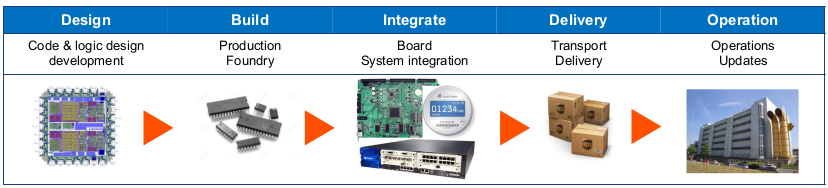
\includegraphics[width=0.7\linewidth]{figures/supply_chain}
	\caption{A globalized production system supplies the components}
	\label{fig:supplychain}
\end{figure}

Nowadays, the production of electronic devices goes through many different stages and hands - there's almost no single company that handles their supply chain end-to-end. Many tiers limit visibility and make it impossible to track the origins of all individual components.

\textbf{Cyber supply chain - points of compromise:}

\vspace{-\topsep}
\begin{itemize}
	\setlength{\itemsep}{0pt}
	\setlength{\parskip}{0pt}
	\item \textbf{Manufacturer:} at will, forced by law, compromised by sub supplier, "unknown" vulnerability, bad features/ accounts, kill switch
	\item \textbf{Third party:} intercept in-transit, change components, hardware implants, modified chips or firmware
	\item \textbf{Operator:} software updates, insecure operations, compromised environment, firmware update, compromised mngt system, insecure link
\end{itemize}
\vspace{-\topsep}

There is a long history of supply chain attacks by nation states as well as by organized crime.

\subsection{Blind spot}

Supply chain attack - scenarios and exposed sectors:

\vspace{-\topsep}
\begin{itemize}
	\setlength{\itemsep}{0pt}
	\setlength{\parskip}{0pt}
	\item Critical systems and devices are \textbf{compromised upon delivery}.
	\item Functionality of critical systems \textbf{changes over time / externally controlled}.
	\item Operation of critical systems \textbf{depend on external services} (cloud, vendor).
	\item Lack of update-functionality results in \textbf{loss of control}.
\end{itemize}
\vspace{-\topsep}

Software vulnerabilities have been known for a long time and are known terrain. Hardware is much less protected \textit{and} it's much harder to detect compromised hardware.

We can differentiate:

\vspace{-\topsep}
\begin{itemize}
	\setlength{\itemsep}{0pt}
	\setlength{\parskip}{0pt}
	\item Targeted attack (industry specific): Targeting non consumer grade products for specific industries. A single component has critical implications for a targeted sector. For example special network equipment (ISP router), ICS, IIOT devices, ...
	\item Opportunistic attack (off the shelf commodity): Targeting off the shelve commodity products for consumers and industry. Only a large number of compromised components become critical. For example computers, logic boards, TVs, home control system, ...
\end{itemize}
\vspace{-\topsep}

\subsection{Impact of compromised hardware of firmware}

Cyber security remained largely software focused in the last few years. However, the impact of compromised hardware is tremendous: compromised hardware or firmware nullifies all other security measures. Hardware or firmware compromise can possibly allow:

\vspace{-\topsep}
\begin{itemize}
	\setlength{\itemsep}{0pt}
	\setlength{\parskip}{0pt}
	\item Remotely access \& control the system
	\item Exfiltrate or leak sensitive information
	\item Disable/cripple functionality, create incorrect results
	\item Enforce the use of insecure algorithms
	\item Physically kill the system
\end{itemize}
\vspace{-\topsep}

Hardware attacks are harder to conduct since far fewer people have the skills and access. \textit{But} they are also much harder to defend since hardware is extremely complex and replacing corrupted hardware can be extremely difficult and expensive.

\textbf{Example: The Chip Design Ecosystem: More Globalized, More Complex}\\
In the earliest days, a single company would produce chips from specification to shipment. Few companies like IBM, Intel, Samsung, and Texas Instruments still do this. Most companies however send their designs to an external facility known as a “foundry” for manufacturing. Designs are provided to manufacturers as descriptions of the shapes and locations of all the silicon and metal structures that must be built into the chip.\\
A skilled attacker could: Compromise a design \& minimizing the chance of detection (chips are so complex that testing is only partial), introduce a flaw with plausible deniability (characterizing the back door as a feature to assist in testing early prototypes of the chips). Statistically, there are enough people with the skills, access, and motivation to intentionally compromise a chip design.\\

The current approach to supply chain security still largely reflects a decade-old view that the most significant vulnerabilities lie in manufacturing. This is no longer the case. As chip complexities have increased, the vulnerabilities have expanded upstream in the supply chain, to include design.

\subsection{Possible approaches to make things better}

We have to do the cyber equivalent of transport safety norm, crash test dummies and periodic/ surprise inspections. Enforce requirements through independent and realistic testing. Build realistic testing capability, including reverse engineering of firmware and hardware.

\subsection{The Great Hack}

Supermicro’s server motherboards in use in many big US tech companies (notably, Apple and Amazon
among them) allegedly contained an hardware implant, designed by Chinese military, that allowed for remote infiltration. The implant was connected to the BMC, Baseboard Management Controller, which sits at a lower level respect to the OS, and runs a separate firmware (on a separate CPU) in order to allow remote administration operations, like reinstalling the OS or restarting an unresponsive machine. The implant would have all the capabilities the BMC has - which is to say, full access to the entire machine. The implant can be directly connected to the Ethernet controller, therefore it would be completely transparent to the the operating system. It is unclear if this attack really happened and if China was actually behind it. However, such supply chain attacks \textit{have} happened before, e.g. by the Persistence Division of NSA’s Tailored Access Operations unit.\\
Note that not only server hardware has BMCs for remote code execution - modern laptops have the same technology.

\section{Probabilistic Traffic Monitoring}

Network traffic monitoring is crucial in today's internet. Applications of traffic monitoring are broad: anomaly detection (detect DoS attack or port scans, enforce QoS), network management (accounting (often deterministic monitoring), usage-based pricing, traffic engineering). Without network management, we have no idea what's happening inside the network.\\
Large content providers such as Google, Akamai, Cloudflare constantly monitor their network to detect large traffic loads and (D)DoS attacks.\\
Why do we want probabilistic monitoring? It's more efficient.
Why do we want deterministic monitoring for accounting? Accounting happens at the edge of the network there we have enough compute power to store all states.\\

Traffic monitoring can be done at different granularities:

\vspace{-\topsep}
\begin{itemize}
	\setlength{\itemsep}{0pt}
	\setlength{\parskip}{0pt}
	\item Per-flow basis: \textit{(srcIP, dstIP, srcPort, dstPort, protocol)}, or IPv6 flow label (20 bit)
	\item Can also monitor on a subset of the flow 5-tuple: DDos detection: \textit{(*, dstIP, *, *, *)}, source bandwidth monitoring for usage-based pricing: \textit{(srcIP, *, *, *, *)}
\end{itemize}
\vspace{-\topsep}

Traffic monitoring is difficult:

\vspace{-\topsep}
\begin{itemize}
	\setlength{\itemsep}{0pt}
	\setlength{\parskip}{0pt}
	\item Core routers in the Internet forward multiple	terabit of traffic per second
	\item Empirical evidence: 20 million different flows on	a 1 Tbps router
	\item On a 1Tbps router we have one packet every \textit{10ns}! (1KB packets)
	\item Monitoring is especially important when something goes wrong (e.g. attacks). Exactly then it's even more challenging since we have more traffic.
	\item Attackers can craft traffic to target monitoring system (send from various ports, spoof srcIP), e.g. to exhaust state of monitoring system
\end{itemize}
\vspace{-\topsep}

\subsection{Basic Concepts of Probabilistic Traffic	Monitoring}

Intuition: trade accuracy/precision for efficiency. Deterministic monitoring is not possible for core internet. Challenge: Measure with limited memory/processing. Output an “accurate” estimate with high probability.

General concept of probabilistic monitoring: (1) Router summarizes traffic into a compact dataset. (2) Router periodically reports the dataset to a server. (3) Server estimates certain statistics based on multiple datasets.\\
(2) \& (3) are optional and not done by all systems.

\subsection{General-Purpose Measurements (NetFlow)}

Sample every packet (standard Netflow) or sample every k-th packet (sampled Netflow). Keep flow entry $\{C_{pkt}, C_{byte}\}$ for each flow, counting the number of sampled packets and bytes.\\ Estimate the number of packets and bytes with $\widetilde{n}_{pkt} = k*C_{pkt}$, $\widetilde{n}_{byte} = k*C_{byte}$.

\newpage

\textbf{Advantages:} simple and efficient.\\
\textbf{Disadvantages:} Memory overhead (one entry per flow in worst case), imprecise estimate, especially for short-lived flows (we have both FP and FN), attacker could exploit by only sending large traffic in between sampling (solution: sample with probability $\frac{1}{k}$)\\

General-purpose flow measurement is either imprecise or infeasible. Solution: focus on specific traffic information (large flows, number of flows, flow distribution, ...).

\subsection{Large-Flow (Elephant) Detectors}

Large flows are flows that consume more than a given threshold of link capacity during a given measurement interval, e.g. flows that take more than 1\% of link capacity. There is evidence that less than 1\% of flows account for more than 90\% of traffic volume. It thus makes sense to look at large flows and ignore small ones.\\
It is possible to efficiently identify large flows without keeping per-flow state on routers because \#large flows $<<$ \#flows in total.

\subsubsection{Sample and Hold (Sampling based)}

This is essentially a variant of Netflow.\\
\textbf{Sample:} We sample each byte with probability p. Practically, samples a packet of size s with probability $p_s$, $p_s = 1-(1-p)^s \approx p*s$ (when p is small).\\
\textbf{Hold:} updates a flow entry for all subsequent packets once it is created. Requires flow-table lookup for every incoming packet. Flow-table stores $\{C_{pkt}, C_{byte}\}$.\\

A problem with sample-and-hold is that for large flows we need to look at all packets. Once we've seen all flows, we might need to keep track of a lot of flows.

\subsubsection{Multistage Filter (Sketch based)}

Use a CountMin sketch to estimate the number of packets of a flow.\\
\textit{Reminder}: CountMin sketches use $k$ different hash function and an array. We hash the flow-tuple with each hash function and increase all counters at the positions indicated by the hash functions. The count estimate is the minimum value of all counters.\\
\textbf{Properties}: fixed memory resources, no FNs (we can't undercount), low FPs (overcount due to hash collisions). However, we need to look at all packets, but we can keep fewer counters.

\subsubsection{EARDet Algorithm (Frequent item finding)}

\textbf{Goal}: Find all flows with $k$ highest packet counts among $m$ flows.\\
\textbf{Algorithm:} We have $k$ counters. For each new packet $p \in f$ (flow $f$), we increase the corresponding counter for $f$ by the packet size. If no counter tracks $f$, we start tracking it. If all counters are used, we decrease \textit{all} counters by the packet size. If one counter reaches zero while decreasing, we add the current flow with the remaining packet size.\\
\textbf{Virtual traffic:} Use “virtual flows” for each idle period. Each virtual flow is at most equal to a low-bandwidth threshold ($Th_L$).\\

\textbf{Properties of EARDet:} no FN for large flows, no FP for small flows, FN \& FP possible for medium flows, deterministic (keep performance regardless of input traffic or attack pattern), relatively small storage cost (but many counters are needed)
\textbf{Disadvantage}: per-packet counter update is an expensive operation

\newpage

\begin{figure}[t!]
	\centering
	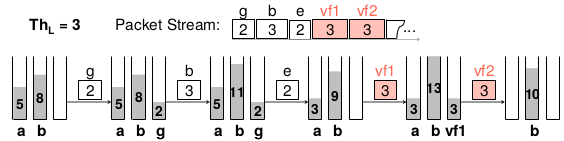
\includegraphics[width=0.5\linewidth]{figures/eardet_algorithm}
	\caption{EARDet Algorithm}
	\label{fig:eardetalgorithm}
\end{figure}

EARDet is an adaption of the MG-algorithm, instead of increasing counters by number of packets, we increase counters by packet size.

\subsection{Finding Duplicates: Bloom Filters}

\textbf{Problem}: identify if an element is a duplicate\\
\textbf{Challenge}: cannot store all previous elements\\
\textbf{Solution}: Bloom filter provides probabilistic data structure for set membership testing\\

Bloom filters are a more memory-efficient approach for insertions and membership queries. Bloom filters consist of a fixed size table \texttt{bf} with $M$ 1-bit cells and $K$ hash functions and we write a 1 at each position indicate by each hash function.

\begin{figure}[hb]
	\begin{minipage}[t]{.5\textwidth} 
		\vspace{0pt}
		\centering 
		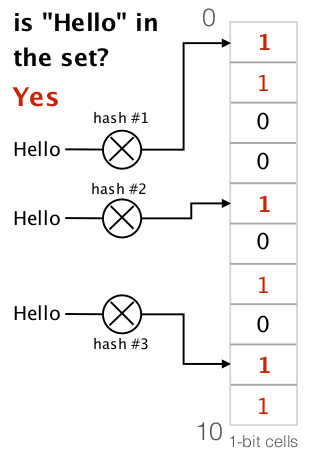
\includegraphics[width=0.45\textwidth]{figures/bloom_filter}
		\caption{Bloom filter \cite{advnet}}
		\label{fig:bloom_filter}
	\end{minipage} 
	\begin{minipage}[t]{.5\textwidth} 
		\vspace{10pt} 
		\begin{itemize}
			\setlength{\itemsep}{0pt}
			\setlength{\parskip}{0pt}
			\item Insert \textit{e} into \texttt{bf}: 
			\begin{enumerate}
				\item $\forall i \in [1,K]$, calculate $h_i(e)$
				\item $\texttt{bf}[h_i(e)] = 1, \forall i \in [1,K]$
			\end{enumerate}
			\item Membership query \textit{e}:
			\begin{enumerate}
				\item if $\texttt{bf}[h_i(e)] == 1, \forall i \in [1,K]$ 
				\newline $\rightarrow$ $e$ is in \texttt{bf}
				\item else 
				\newline $\rightarrow$ $e$ is not in \texttt{bf}
			\end{enumerate}
		\end{itemize}
	\end{minipage} 
\end{figure}

\subsubsection{Dimension your bloom filter}
\label{bloom_filter_dimension}

$N$ elements, $M$ cells, $K$ hash functions, $FP$ false positive rate.

\vspace{-\topsep}
\begin{itemize}
	\setlength{\itemsep}{0pt}
	\setlength{\parskip}{0pt}
	\item probability that one hash function returns the index of a particular cell: $\frac{1}{M}$
	\item probability that one hash function does not return the index of a particular cell: $1 - \frac{1}{M}$
	\item probability of a cell to be 0: $(1 - \frac{1}{M})^{KN}$
	\item false positive rate P(FP): $(1 - (1 - \frac{1}{M})^{KN})^K$
	\item false negative rate: 0
\end{itemize}
\vspace{-\topsep}

For an approximation, use: $p := P(FP) = (1 - (1 - \frac{1}{M})^{KN})^K \approxeq (1 - e^{-KN/M})^K$.\\

There's a global minimum when $K = \ln(2) * \frac{M}{N}  \approx 0.7*\frac{M}{N}$ found by taking derivative of $P(FP)$.\\
For that choice of $K$, resulting $p := P(FP) = 2^{-K} \approx 0.6185^{M/N}$.\\
Given optimal $K$, choice of optimal $M = -\frac{N \ln p}{(\ln2)^2}$ $\rightarrow O(N)$ space.

\newpage

\textbf{In practice:} if we use the Bloom filter for a long time, it's going to fill up, which leads to more false positives (a full bloom filter we just conclude that every packet is in the filter). We thus need to reset the Bloom filter periodically. Simply resetting the whole Bloom filter leads to false negatives (all cells are back to 0 after reset).\\
In practice, we use \textit{two} same-sized Bloom filters and alternate them. We only put values into one single BF at a time and switch after a reset. \textit{BUT} for membership queries, we always check both filters! However, for very old packets we can still get FNs. Solution: use timestamps on packets and remove tracking for old packets. This gives us the FN guarantee.

\subsection{Probabilistic Counting: Estimating the Number of Flows}

\textbf{Simple probabilistic counting:} Hash flow ID to generate a value in [0,1). Keep the flow ID associated with the smallest hash value.\\
Expectation value of smallest value is 1 / (number of flows + 1).\\
Estimate the number of flows by the smallest value v seen so far: $\tilde{n} \approx 1/v - 1$.\\

\textbf{Problems:}
\vspace{-\topsep}
\begin{itemize}
	\setlength{\itemsep}{0pt}
	\setlength{\parskip}{0pt}
	\item minimum has large variance $\rightarrow$ not very robust
	\item An attacker controlling only 1 input can bias the estimation. Solution: use private hash function or salted hashing.
\end{itemize}
\vspace{-\topsep}

\textbf{Proposal by Bar-Yossef et al. (2002):}

\vspace{-\topsep}
\begin{itemize}
	\setlength{\itemsep}{0pt}
	\setlength{\parskip}{0pt}
	\item Keep track of the $k$ smallest hash values
	\item Expectation value of $k$-th smallest value is $k/(n+1)$, variance is smaller
	\item Estimate the number of flows by the k-th smallest value $v_k$ that has been seen
	so far: $\tilde{n} \approx k / v_k - 1$
\end{itemize}
\vspace{-\topsep}

\subsection{Traffic Monitoring vs. Intrusion Detection}

Both can detect malicious activities such as DoS attacks \& port scans at selected network
vantage points.\\
\textbf{Intrusion detection:} Typically deployed at network edges, destination-based diagnosis, can analyze detailed payload data as well.\\
\textbf{Traffic monitoring:} Can be deployed at high-speed backbone routers, diagnoses network-wide anomalies, analyzes packet headers only.

\section{Border Gateway Protocol (BGP) Security}

Why should we care about BGP security when we have secure connections (TLS, VPN, DNSSEC, etc.)? The one that controls BGP controls routing. A \textit{lot} can be exploited when controlling routing.

\vspace{-\topsep}
\begin{itemize}
	\setlength{\itemsep}{0pt}
	\setlength{\parskip}{0pt}
	\item Obtain fake TLS certs: use BGP route hijacking in combination with automatic certificate issuance (ACME) to obtain fake TLS certs. BGP allows to reroute HTTP challenge traffic from CA to illegitimate IP.
	\item deanonymize TOR users: reroute TOR exit node traffic and use it for correlation attacks.
	\item hijack DNS requests: hijack routes to DNS servers (e.g. MyEtherwallet hack)
	\item partition the Bitcoin network
\end{itemize}
\vspace{-\topsep}

The problem with BGP is that endusers can't protect themselves. Solving these issues is only possible with ISP cooperation.

\newpage

\textbf{BGP vs. OSPF:} BGP is used as an inter Autonomous System protocol, while OSPF is used to establish routes inside an AS. Also, OSPF is a link-state protocol: routers exchange what they know about the network until all routers have a complete map of the network; then the routers compute the routing tables independently. In BGP, we have a path-vector mechanism: every AS announces the prefixes it owns and all the paths that go through it to neighboring ASes.

\subsection{IP Addresses, Autonomous Systems \& the Border Gateway Protocol}

\textbf{IP addresses:} are globally assigned by ICANN (global authority). ICANN assigns certain IP regions to certain parts of the world. Regional Internet Registries (RIRs) are then responsible to further assign IPs. As of 25th November 2019 15:35 UTC+1, we have officially run out of IPv4 addresses.\\
IP addresses are assigned in prefixes (e.g. /16 prefix has $2^{32-16} - 2= 65534)$ IPs).\\

\textbf{Internet:} The Internet is a network of networks (autonomous systems). Autonomous systems can be ISPs (e.g. DT, Swisscom), global backbone network (e.g. Verizon), universities and large companies (e.g. ETH, Google).\\

\textbf{BGP:} BGP "glues" the internet together: routing protocol between ASes, disseminates information about location and paths for IP prefixes. BGP is a path-vector protocol and follows typical business relationships.\\
BGP speaker sends and receives messages from peers over TCP connections on port 179. Messages sent include: \texttt{OPEN, UPDATE, KEEPALIVE, NOTIFICATION}. Route information is disseminated through \texttt{UPDATE} message using attributes: \texttt{Withdraw, path attributes, network layer reachability information}.\\

\begin{figure}
	\centering
	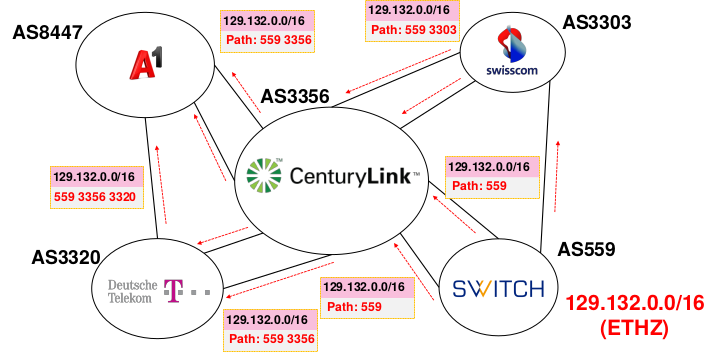
\includegraphics[width=0.6\linewidth]{figures/bgp_ases}
	\caption{The Internet is a network of networks (ASes). BGP “glues” these systems together. ASes exchange information about IP prefixes they can reach directly or indirectly}
	\label{fig:bgpases}
\end{figure}

\textbf{BGP route selection criteria:}

\vspace{-\topsep}
\begin{enumerate}
	\setlength{\itemsep}{0pt}
	\setlength{\parskip}{0pt}
	\item higher LOCAL-PREF
	\item Shorter AS-Path length
	\item lower MED (value is set by the business partner and used to express his preference)
	\item prefer learned over eBGP instead of iBGP (hot-potato routing)
	\item smallest ingress IP address (used as tie-breaker)
\end{enumerate}
\vspace{-\topsep}

\newpage

ASes have different business relationships with each other: provider, peer, customer. Each AS implements peering policies. These decide routes are accepted and advertised based on policies. Policies are configured in the BGP daemons of the AS. Policies can be used to implement filters to prevent route leaks (= falsely announced prefixes), or for business reasons.

\vspace{-\topsep}
\begin{itemize}
	\setlength{\itemsep}{0pt}
	\setlength{\parskip}{0pt}
	\item Input policy: which paths to keep/ discard
	\item Export policy: which paths do I advertise to neighbors
\end{itemize}
\vspace{-\topsep}

\subsection{BGP Hijacks}

BGP was designed during the early days of the internet - security was of no concern back then. BGP faces many security problems: Lack of authentication for advertisements and lack of verification of the advertised information. Slow convergence makes it hard to provide availability guarantees on the Internet.

\subsubsection{Problem 1: BGP does not validate the origin of advertisements}
\label{bgp_problem_1}

If I advertise some prefix as mine, BGP will \textit{not} check if I actually own that prefix.\\
This allows malicious ASes to hijack prefixes: assume AS V owns prefix \textit{v} (129.132.0.0/16). Malicious AS M can just advertise \textit{v} as well and since there is no validation, other ASes don't know which one is the correct advertisement.  Some ASes will thus pick the malicious advertisement (selection based on properties such as AS path length). However, ther is an even stronger version of this:\\

\textbf{Sub-Prefix Hijacking:} AS M can announce a \textit{more specific} prefix for the victim's (AS V) address space (up to /24 is allowed). AS M could announce two /17 prefixes for V's prefix 129.132.0.0/16. Since routing in the internet is based on longest prefix matching, \textit{all} routers will pick the more specific prefix.\\
Prefixes up to /24 are allowed - always announcing /24 prefixes as protection doesn't work since (a) routing tables would become huge and (b) BGP routers would probably merge the prefixes anyway.

\begin{figure}
	\centering
	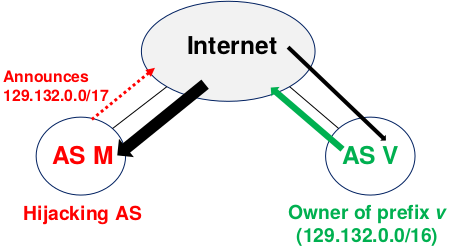
\includegraphics[width=0.4\linewidth]{figures/bgp_subprefix_hijack}
	\caption{BGP Sub-Prefix Hijacking}
	\label{fig:bgpsubprefixhijack}
\end{figure}

\textbf{What can be done to the hijacked traffic?}

\vspace{-\topsep}
\begin{itemize}
	\setlength{\itemsep}{0pt}
	\setlength{\parskip}{0pt}
	\item Blackhole (just drop traffic)
	\item Redirect: send to other destination (e.g. for analysis)
	\item Intercept: analyze and then send traffic to correct destination (traffic just takes a detour). This is actually not that easy since the attacker needs to be able to handle the traffic, which can be difficult for high-volume victims.
\end{itemize}
\vspace{-\topsep}

BGP interception can be made more sophisticated:

\vspace{-\topsep}
\begin{itemize}
	\setlength{\itemsep}{0pt}
	\setlength{\parskip}{0pt}
	\item Only announce the bogus advertisement to selected neighbors (but others might still learn the route from their peers)
	\item Use BGP communities to explicitly state to which ASes a particular advertisement should be advertised.
\end{itemize}
\vspace{-\topsep}

BGP hijacking is not as easy as it sounds (you can't just announce route from your home router). You need access to a BGP router (your own AS or compromised AS).

\subsection{Problem 2: BGP does not validate the content of	advertisements}

After a BGP message has been announced, the content of the advertisement is not validated! ASes that receive the advertisement can modify it!

\textbf{ASes can modify the BGP path:}

\vspace{-\topsep}
\begin{itemize}
	\setlength{\itemsep}{0pt}
	\setlength{\parskip}{0pt}
	\item Remove ASes from the AS path:\\
	Legitimate AS Path: [AS 701, AS 6939, AS 88]. Remove AS 6939: [AS 701, AS 88]\\
	\textbf{Motivation:}
	\vspace{-\topsep}
	\begin{itemize}
		\item 	Attract traffic by making path look shorter, attract sources that try to avoid\\
		AS 6939.
	\end{itemize}
	Only AS 701 can tell that the AS path is wrong!
	\item Add ASes to the AS path:\\
	Legitimate AS Path: [AS 701, AS 88]. Add 6939 in-between: [AS 701, AS 6939, AS 88]\\
	\textbf{Motivation:}
	\vspace{-\topsep}
	\begin{itemize} 
		\item Trigger loop detection in AS 6939 (AS sees itself on the AS path and drops the advertisement to avoid routing loops) $\rightarrow$ DoS attack on AS 6939, "BGP poisoning".
		\item Make your AS look like it has richer connectivity
	\end{itemize}
	AS 701 can detect the AS path is wrong (but may not care), AS 6939 could detect but may not see the route.
\end{itemize}
\vspace{-\topsep}

\begin{figure}
	\centering
	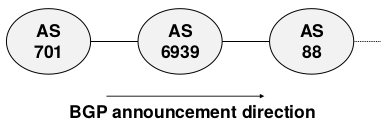
\includegraphics[width=0.4\linewidth]{figures/bgp_as_path}
	\caption{ASes can modify the BGP path}
	\label{fig:bgpaspath}
\end{figure}

\subsection{Attacks on BGP: Obtaining fake certificates}

When using ACME (Automated Certificate Management Environment), a domain is validated through either a HTTP challenge or a DNS challenge to prove that you actually own the domain. By using BGP hijacking, an attacker can:

\vspace{-\topsep}
\begin{itemize}
	\setlength{\itemsep}{0pt}
	\setlength{\parskip}{0pt}
	\item hijack the DNS request of the CA $\rightarrow$ the CA will get a wrong IP owned by the attacker.
	\item hijack the connection to the correct IP and route it to an IP she owns.
\end{itemize}
\vspace{-\topsep}

Read \cite{bgp_fake_cert} for more information.

\subsection{Other attacks on BGP}

\begin{itemize}
	\setlength{\itemsep}{0pt}
	\setlength{\parskip}{0pt}
	\item Denial-of-service attacks: overload links between BGP routers, send bogus TCP packets (FIN/RST to close session, TCP SYN flood)\\
	A possible solution to bogus TCP RST is to only accept TCP RST with TTL=255, i.e. only TCP RST from direct neighbor router.
	\item Eavesdrop or tamper messages by tapping the link
	\item Most such attacks are easy to defend against and are no longer a large concern
\end{itemize}
\vspace{-\topsep}

\newpage

\subsection{Countermeasures}

\subsubsection{Best Current Practices (BCPs)}

BCPs are essentially "gentlemen's agreement" between ASes. ASes promise to apply them but there are no guarantees:

\vspace{-\topsep}
\begin{itemize}
	\setlength{\itemsep}{0pt}
	\setlength{\parskip}{0pt}
	\item Securing the BGP peering session between routers (authentication, prioritize BGP traffic)
	\item Filtering routes by prefix and AS path
	\item Filters to block unexpected control traffic (e.g. ignore TCP RST for BGP if it comes from the inside, implement TTL=255 policy)
	\item Enter prefixes int Internet Routing Registries (IRRs) and filter based on these entries
\end{itemize}
\vspace{-\topsep}

None of these actually have strong security properties (no crypto).

\subsubsection{Origin Authentication (OA) (solution to \ref{bgp_problem_1})}

OA uses a Resource Public-Key Infrastructure (RPKI) to prove ownership of resources. The RPKI is a “secure database” to map Internet number resources to a trust anchor. Every AS owned prefixes is now registered in the RPKI, s.t. the authenticity of prefix announcements can be verified. 
%A digital certificate proves that an AS is the current holder of a specific resource. 
RIRs are trust roots.\\
This enables issuance of Route Origination Authorizations (ROAs): state which AS is authorized to advertise certain IP prefixes, determine the max length of a prefix (avoid sub-prefix hijacking). Certs follow the same delegation as IP addresses from RIRs. OA requires no actual modification to BGP. Trusted local caches collect information from RPKI servers and whitelists are periodically pushed to routers: the verification of signatures is therefore performed offline.\\

If AS M now tries to hijack AS V's prefix $v$, routers will check against ROAs in RPKI for prefix $v$ and see that the announcement is invalid and thus drop it.\\
\textbf{However}, AS M can announce that it has a path to AS V by appending itself on the path \textit{after} the entry for AS V. BGP routers in other ASes check against ROAs in RPKI for prefix $v$, and find a valid ROA for prefix $v$. AS M manages to attract a fraction of traffic for AS V.

\begin{figure}
	\centering
	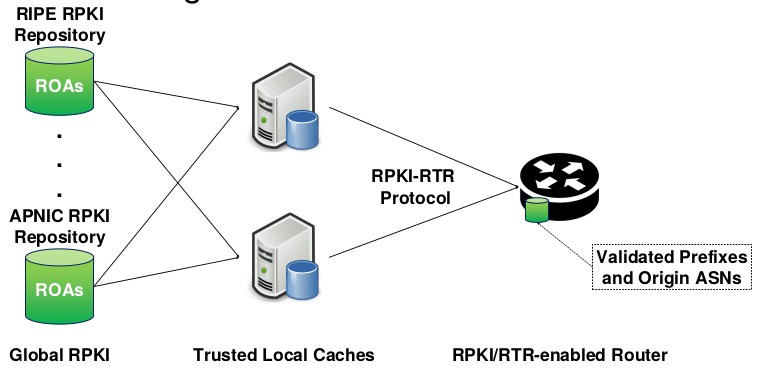
\includegraphics[width=0.5\linewidth]{figures/origin_authentication}
	\caption{Origin Authentication in an ISP}
	\label{fig:originauthentication}
\end{figure}

\begin{figure}[b!]
	\centering
	\begin{subfigure}[t]{.5\textwidth}
		\centering
		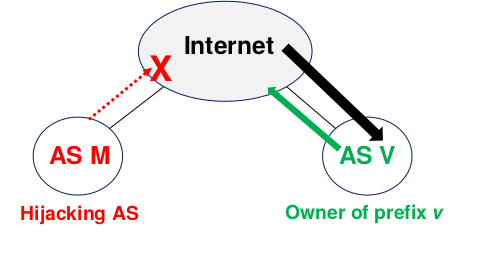
\includegraphics[width=0.7\linewidth]{figures/bgp_oa_as_1}
		\label{fig:bgp_oa_as_1}
	\end{subfigure}%
	\begin{subfigure}[t]{.5\textwidth}
		\centering
		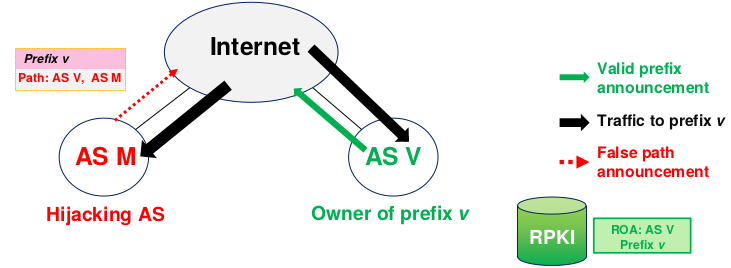
\includegraphics[width=1.1\linewidth]{figures/bgp_oa_as_2}
		\label{fig:bgp_oa_as_2}
	\end{subfigure}
	\caption{Origin Authentication helps but is not enough}
\end{figure}

\subsubsection{BGPsec}

In order to prevent the problem of ASes illegitimately appending themselves to AS paths, we need to secure the AS-path attribute, which prevents crafting a valid origin on path and path poisoning. BGPsec is trying to achieve this through Origin authentication and cryptographic signatures.\\
BGPsec signs received update message to prove that path was correctly updated and includes the next AS in the signature. This way, BGPsec can validate that the AS path indicates the order ASes were traversed and that no intermediate ASes were added or removed. RPKI is used to verify AS key material (as in origin authentication).\\

Example, figure \ref{fig:bgpsec}: AS 701 send out advertisement and signs msg with its privatekey. AS 6939 can verify the signature (pubKey of AS 701) and add the next AS to the path and again sign the message. ASes always need include the next AS on the path and then sign - otherwise there would be no link between ASes and only individual ASes are secured but not the linking between them.

\textbf{Problems:}

\vspace{-\topsep}
\begin{itemize}
	\setlength{\itemsep}{0pt}
	\setlength{\parskip}{0pt}
	\item Insecure ASes use legacy BGP, and secure ASes must accept legacy insecure routes $\rightarrow$ \textit{protocol downgrade attacks}: If operators don’t prioritize security, an attacker can just use legacy BGP to announce bogus routes to BGPsec neighbors.
	\item Routing policies can interact in ways that can cause BGP wedgies.
	\item \textit{Performance degradation}: Prefix aggregation no longer possible, since you can't sign a prefix owned by someone else. Real-time signature and validation. Slower convergence.
	\subitem $\rightarrow$ \textit{BGPsec does not scale}
\end{itemize}
\vspace{-\topsep}

\begin{figure}
	\centering
	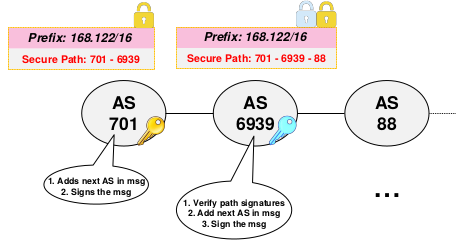
\includegraphics[width=0.5\linewidth]{figures/bgpsec}
	\caption{BGPsec : Secure Version of BGP}
	\label{fig:bgpsec}
\end{figure}

\subsubsection{Path-End Validation: Deployable Routing Security}

Important observation: AS paths today are very short! Average AS-level path length is only 3-4 hops. The basic idea is to have something between origin authentication and BGPsec. Path-End Validation tries to reduce overhead of BGPsec.\\

\vspace{-\topsep}
\begin{itemize}
	\setlength{\itemsep}{0pt}
	\setlength{\parskip}{0pt}
	\item Origin Authentication with RPKI secures only the announced prefix. This way, no AS can announce a prefix it does not own.
	\item Path-end Validation secures the first hop	from originator to its provider. This way, no AS can simply append itself after the first AS on the AS path. Why does this work: you can still append yourself after two ASes. \textit{But} this makes the AS path rather long and thus less attractive.
\end{itemize}
\vspace{-\topsep}

This has several advantages over full BGPsec: Lower overhead, requires no cooperation from other ASes, no full deployment necessary, stronger incentive for early adopters.

\newpage

\subsection{Famous BGP hijacks}

\subsubsection[Pakistan trying to censor Youtube]{Pakistan trying to censor Youtube \footnote{\href{https://www.ripe.net/publications/news/industry-developments/youtube-hijacking-a-ripe-ncc-ris-case-study}{https://www.ripe.net/publications/news/industry-developments/youtube-hijacking-a-ripe-ncc-ris-case-study}}}

The Youtube AS was announcing his owned IP subnet 208.65.152.0/22. The Pakistani national telecom provider started announcing 208.65.153.0/24 in an attempt to override the legitimate definition for censorship purposes. The override was successful because this is a sub-prefix, meaning the longest prefix matching would prefer the /24 subnet. The mistake was announcing the route also to their upstream provider: the path was then propagated to the whole Internet, bringing down the Youtube website worldwide.\\
Youtube tried to announce a longer prefix. Originally it announced a /24 subnet, which was only partially effective, and it finally announced two /25 subnets, which were preferred by most routers. This is not always possible, as announcing all the prefixes would surely be detrimental to network throughput. Additionally, the separate more specific announcements may be aggregated by routers receiving the message for convenience.

\subsubsection[Russia hijacking financial organizations]{Russia hijacking financial organizations \footnote{\href{https://bgpmon.net/bgpstream-and-the-curious-case-of-as12389/}{https://bgpmon.net/bgpstream-and-the-curious-case-of-as12389/}}}

The Russian Telecom company Rostelecom started advertising 50 prefixes as own. The mix of organizations is interesting: from Verisign to Visa, Mastercard, HSBC and other financial institutions.

\newpage

\section{SCION \small (Secure Multipath Interdomain Routing Architecture)}

BGP security issues have been going on for years. Instead of trying to fix and patch BGP, why not just develop a completely new inter-AS protocol with modern requirements as features.\\

\textbf{Goals of SCION:} High availability, Secure entity authentication, Flexible trust, Transparent operation, Balanced control, Scalability, efficiency

\subsection{Control plane: How to find end-to-end paths?}

The architecture of SCION mandates that the Internet is partitioned into \textit{Isolation Domains (ISDs)}, that are independently organized groupings of ASes. In each ISD, part of the ASes form the \textit{ISD core}, which is responsible for managing the whole ISD and has some special functions (e.g. Swisscom, Sunrise would be core ASes). An ISD usually represents an area of common trust or of common legislation (e.g. countries, multinational federations). ISDs are SCION's approach for scalability and they are a virtual concept: ASes can be in different ISDs and can have different roles in different ISDs.

\subsubsection{Intra-ISD Path Exploration: Beaconing}

Beaconing is am asynchronous process through which paths are found in SCION. The Core ASes in an ISD (Isolation Domain) periodically flood the ISD with PCBs, by sending them in an anycast fashion (dubbed service anycast in SCION). Any AS receiving this packet will send it to its beacon server, which will add the current AS info and send the PCB to the ASes downstream. When beacons reach leaf nodes in the AS graph, the process is completed. Each AS receives multiple PCBs representing path segments to a core AS.\\

Each AS deploys one or multiple beacon servers. SCION border routers receive PCB
and select one beacon server to forward it to. Beacon servers coordinate to resend PCBs periodically to downstream ASes (currently every 5 seconds). ASes can choose to which customers and peers to forward which beacons, but in the end it is the sources that determine the final path.\\

\textbf{PCB contents:} PCB contains an info field with: PCB creation time. Each AS on path adds: AS name, Hop field for data-plane forwarding (Link identifiers, Expiration time, Message Authentication Code (MAC)), AS signature.\\
\textit{Link identifier}: ASes have multiple interface numbers. The hop field has an \texttt{IN} and \texttt{OUT} link identifier, they say where traffic enters/ leaves the AS.\\
\textit{MAC}: highly efficient (verified in a few ns) but needs symmetric keys (only known inside the AS). This allows the AS to verify its own forwarding information.

\begin{figure}[hb]
	\centering
	\begin{subfigure}[t]{.5\textwidth}
		\centering
		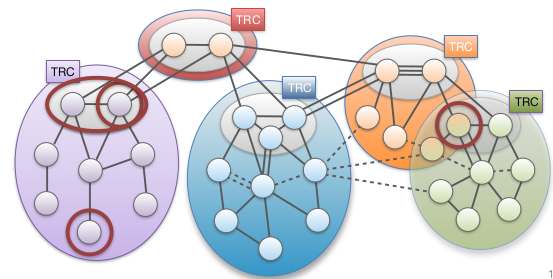
\includegraphics[width=0.7\linewidth]{figures/scion_isd}
		\label{fig:scion_isd}
		\caption{Approach for Scalability: ISDs}
	\end{subfigure}%
	\begin{subfigure}[t]{.5\textwidth}
		\centering
		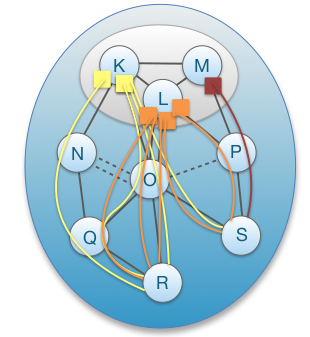
\includegraphics[width=0.4\linewidth]{figures/scion_beaconing}
		\label{fig:scion_beaconing}
		\caption{Intra-ISD Path Exploration: Beaconing}
	\end{subfigure}
	\caption{}
\end{figure}

\newpage

\textbf{Up-Path and Down-Path Segments:} PCBs contain path segments that
can be used as communication paths. A path segment is any contiguous subsequence of ASes contained in a PCB, provided that at least one of the extremes is a core AS. They owe their name to the fact that they represent different segments of a whole path. Each path is comprised of an \textbf{up-path segment} (from source AS to a core AS) plus a \textbf{core-path segment} (from core AS to core AS, possibly on a different ISD), plus a \textbf{down-path segment} (from core to destination AS).\\

\subsubsection{Core Beaconing for Inter-ISD Path Exploration}

Beaconing that happens inside ISDs also happens across ISDs $\rightarrow$ core ASes beacon among each other. Beacon info looks similar as for intra ISD beaconing. With Core Beaconing for Inter-ISD Path Exploration, there is \textit{no} convergence process! Connecting the whole internet would only take a few seconds. However, finding the best and multiple paths takes longer.\\
\textit{But:} scalability of inter-ISD beaconing is actually \textbf{worse} than in BGP because we send lots of inter-ISD beacons and we also want to discover multiple paths. However, it still scales since the number of core ASes is highly limited (few tier 1 Ases).

\subsubsection{Path server infrastructure}

Every AS has its own path server. Non-core AS's path server contains up-path segments to reach the core ASes. Core AS's path server contains down-path segments and core-path segments. Caches along the way cache paths at various levels.\\
\textbf{Up-Path Segment Registration:} AS selects path segments to announce
as up-path segments for local hosts. Up-path segments are registered at local path servers.\\
\textbf{Down-Path Segment Registration:} AS selects path segments to announce as down-path segments for others to use to communicate with AS. Down-path segments are uploaded to core path server in core AS.

\subsection{Data plane: How to send packets}

In IP, the router looks up a routing table and (usually based on the destination of the packet) makes a routing decision, forwarding the packet to the appropriate interface. In SCION none of that happens: the packet already contains the forwarding information (full AS path), so a router only needs to check the next hop information in the SCION header. As a consequence, SCION packets need larger headers compared to IP.

\subsubsection{Path lookup}

Disadvantage of SCION over today's internet: we need to look up paths. In today's internet, we just lookup an IP, send a packet and pray.\\

\textbf{Steps of a host to obtain path segments:}

\vspace{-\topsep}
\begin{enumerate}
	\setlength{\itemsep}{0pt}
	\setlength{\parskip}{0pt}
	\item Host contacts RAINS server with a name: H $\rightarrow$ RAINS\\
	RAINS $\rightarrow$ H: ISD X, AS Y, local address Z
	\item Host contacts local path server to query path segments H $\rightarrow$→ PS: ISD X, AS Y\\
	PS $\rightarrow$ H: up-path (to local ISD core ASes), core-path (connect up-path and down-path
	segments), down-path segments (from core AS to ISD X)
	\item Host combines path segments to obtain end-to-end 	paths, which are added to packets\\
\end{enumerate}
\vspace{-\topsep}

\newpage

\textbf{Path lookup: local ISD}\\
In step 2, client requests path segments from local path server. If down-path segments are not cached, local path server sends request to core path server.\\

\textbf{Path Lookup: remote ISD}\\
In step 2, client requests path segments from local path server. If down-path segments are not cached, local path server send request to core path server. If core path server does not have path segments cached, it will contact remote core path server.

\begin{figure}[t!]
	\centering
	\begin{subfigure}[t]{.5\textwidth}
		\centering
		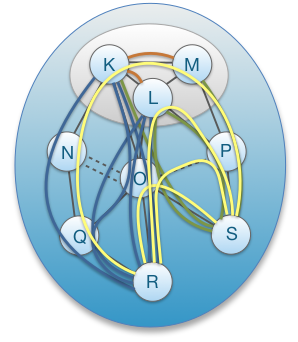
\includegraphics[width=0.5\linewidth]{figures/scion_pathlookup_localisd}
		\label{fig:scion_pathlookup_localisd}
		\caption{Path Lookup: Local ISD}
	\end{subfigure}%
	\begin{subfigure}[t]{.5\textwidth}
		\centering
		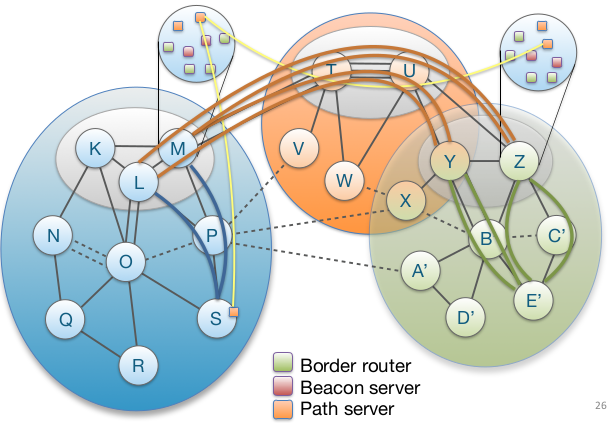
\includegraphics[width=0.7\linewidth]{figures/scion_pathlookup_remoteisd}
		\label{fig:scion_pathlookup_remoteisd}
		\caption{Path Lookup: Remote ISD}
	\end{subfigure}
	\caption{}
\end{figure}

Path segments are valid for several hours and cached locally. Otherwise the whole process would take too much time for each time we want to send. SCION’s path combination of up-path, core-path, and down-path segments reflect current Internet routing.\\

Problem: Economic incentives are not all prevailed in SCION: customer could choose to use a very costly link (path) since we have multiple paths available. This would be bad for the provider. \textit{But:} this could be solved by the provider by setting BW limits or just making customers pay more if they use more expensive links.

\begin{figure}[hb]
	\centering
	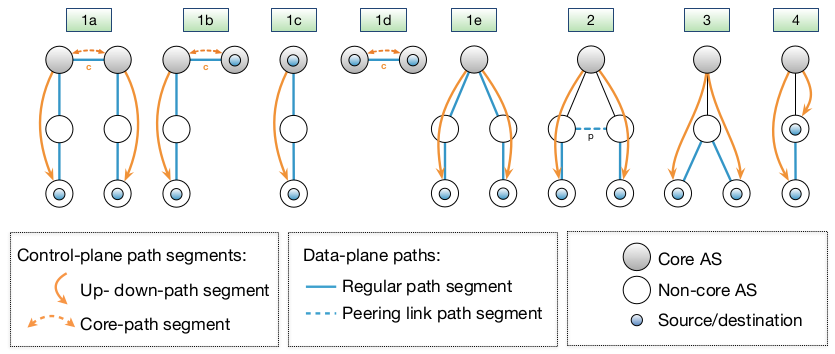
\includegraphics[width=0.8\linewidth]{figures/scion_path_combinations}
	\caption{SCION path combinations}
	\label{fig:scionpathcombinations}
\end{figure}

\newpage

\subsubsection{SCION Packet Header}

A SCION packet has multiple headers:

\vspace{-\topsep}
\begin{itemize}
	\setlength{\itemsep}{0pt}
	\setlength{\parskip}{0pt}
	\item SCION common header
	\item SCION source and destination address
	\item Info field provides information about a path segment
	\item Path segment consists of one or multiple hop fields
\end{itemize}
\vspace{-\topsep}

SCION does not look at srcIP \& dstIP in the network! Only when the packet gets to the destination AS will IPs be considered. \textbf{This allows for communication between private address spaces!} E.g. 192.168.0.1 in AS X could communicate with 192.168.0.1 in AS Y. Also, this would solve IPv4 address exhaustion (although IPv6 already solved it).

\begin{figure}[t!]
	\begin{subfigure}[t]{.5\textwidth}
		\centering
		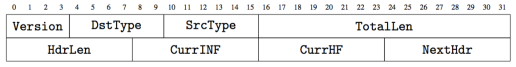
\includegraphics[width=\linewidth]{figures/scion_common_header}
		\label{fig:scion_common_header}
		\caption{SCION common header}
	\end{subfigure}
	\hfill
	\begin{subfigure}[t]{.5\textwidth}
		\centering
		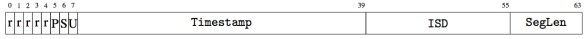
\includegraphics[width=\linewidth]{figures/scion_info_field}
		\label{fig:scion_info_field}
		\caption{SCION info field}
	\end{subfigure}
	
	\medskip
	
	\begin{subfigure}[t]{.5\textwidth}
		\centering
		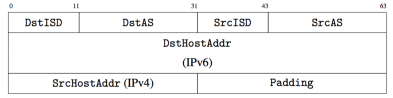
\includegraphics[width=\linewidth]{figures/scion_address_header}
		\label{fig:scion_address_header}
		\caption{SCION source and destination address}
	\end{subfigure}
	\hfill
	\begin{subfigure}[t]{.5\textwidth}
		\centering
		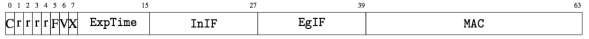
\includegraphics[width=\linewidth]{figures/scion_hop_field}
		\label{fig:scion_hop_field}
		\caption{SCION hop field}
	\end{subfigure}
	\caption{}
\end{figure}

\subsubsection{Ingress and Egress Interface Identifiers}

Each AS assigns a unique integer identifier to each interface that connects to a neighboring A. The interface identifiers identify ingress/egress links for traversing AS. ASes use internal routing protocol to find route from ingress SCION border router to egress SCION border router

\subsubsection{Path Encoding in Packet}

In order to send a packet back (destination to source), we don't need to do another path lookup! The dst just needs to do some parsing to reverse the path. Forward and return paths are the same (one could also lookup a new path).

\begin{figure}[t!]
	\centering
	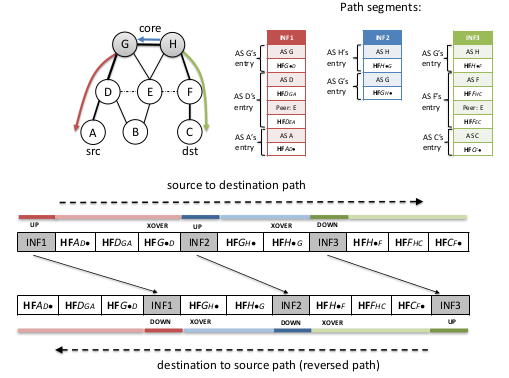
\includegraphics[width=0.7\linewidth]{figures/scion_path_encoding}
	\caption{Path Encoding in Packet}
	\label{fig:scionpathencoding}
\end{figure}

\subsubsection{Hop Field MAC Verification}

Message Authentication Code (MAC) computation and verification of Hop Field MAC value based on local AS secret key (not shared with any external entity).\\
Computation: $MAC_K(Timestamp,Flags’_{HF},ExpTime,Ingress,Egress, HF’)$, with HF the hop field of the previous AS.\\
With AESni HW crypto, only ~30 cycles are needed to compute MAC!

\newpage

\subsection{Deployment and use cases}

\textbf{ISP deployment:} Core ASes have to adapt quite a lot and need to do quite a bit of work for SCION. For regular ASes, most of this work is not needed. Integration of SCION limits to additional infrastructure such as beacon server, path server, RAINS, certificate, SIBRA and time servers.

\subsubsection{Use Case: Low-Latency Connectivity}

Generally, two paths exist between Europe and Southeast Asia: 

\vspace{-\topsep}
\begin{itemize}
	\setlength{\itemsep}{0pt}
	\setlength{\parskip}{0pt}
	\item western route (Europe-US-SEA): High latency, high bandwidth
	\item eastern route (Europe, Suez canal, SEA): Low latency, low bandwidth
\end{itemize}
\vspace{-\topsep}

BGP is a “money routing protocol”, traffic follows cheapest path, typically highest bandwidth path. Thus, Europe-SEA traffic generally takes the western route. There is no wrong path (both have advantages and disadvantages) but the wrong thing to do is to only advertise one single path (as BGP does).

\subsubsection{Use Case: Low Earth Orbit Satellite Networks}

Speed of light in fibres is a lot slower than speed of light in free space. New Low Earth Orbit (LEO) satellite networks only require around 5ms propagation latency between earth and satellite. Inter-Satellite Laser (ISL) links enable global communication. However, LEO has frequent outages/ short time windows of availability due to changing weather conditions - BGP convergence is too slow to support. SCION however can optimally integrate LEO network into Internet fabric.


\newpage

\section{DDoS Attacks and Defenses}
\label{ddos}

Denial of Service (DoS) attack: attempt to consume resources which are then not available to legitimate users. Possible target resources: network links, servers, processing, storage, etc. Distributed Denial of Service (DDoS) attack is a coordinated DoS with many attackers. DDoS attacks pose a significant threat!

\subsection{Attack types}

\subsubsection{Volumetric attacks}

\textbf{Attack:} \textit{Consume the bandwidth} either within the target network/service, or between the target network/service and the rest of the Internet. This causes congestion.\\
\textbf{Metric:} bits/sec\\
\textbf{Typical vectors:}
\vspace{-\topsep}
\begin{itemize}
	\setlength{\itemsep}{0pt}
	\setlength{\parskip}{0pt}
	\item ICMP packet floods (including all ICMP message types)
	\item UDP packet floods
	\item Malformed ICMP, UDP, IP packet floods
	\item Reflection/Amplification
	\item Examples: DNS, NTP, memcached reflection
\end{itemize}
\vspace{-\topsep}

\textbf{Why are volumetric attacks so successful?} Because of TCP. Link flooding causes congestion \& high loss rates for incoming traffic. TCP tremendously slows down under congestion/ packet loss (throughput deteriorates).

\subsubsection{Protocol attacks}

\textbf{Attack:} Designed to \textit{exhaust resources available on the target or on a specific device} between the target and the Internet (e.g. routers, load balancers, security devices). Once the attack consumes a resource such as a device’s TCP state table, no new connections can be opened. Protocol DDoS attacks don't need to consume all of the target’s available bandwidth to make it inaccessible. They can take down even high-capacity devices capable of maintaining state on millions of connections.\\
\textbf{Metric:} packets/sec\\
\textbf{Typical vectors:}
\vspace{-\topsep}
\begin{itemize}
	\setlength{\itemsep}{0pt}
	\setlength{\parskip}{0pt}
	\item SYN/ACK floods, RST attacks
	\item TCP connection floods
	\item Fragmentation attacks
	\item DNS, NTP reflection
\end{itemize}
\vspace{-\topsep}

\subsubsection{Application-Layer Attacks}

\textbf{Attack:} Target various aspects of an \textit{application or service} at Layer 7. Most sophisticated and stealthy attacks as they can be very effective with as few as one attacking machine generating traffic at a low rate. Attacks are very difficult to proactively detect with traditional flow-based monitoring solutions. Application-layer attacks are often referred to as stealthy or low-and-slow attacks.\\
\textbf{Metric:} requests/sec\\
\textbf{Typical vectors:}
\vspace{-\topsep}
\begin{itemize}
	\setlength{\itemsep}{0pt}
	\setlength{\parskip}{0pt}
	\item Layer 7 protocols, HTTP, SMTP, DNS, SNMP, FTP, SIP, etc.
	\item Application request floods
	\item Database connection pool exhaustion
	\item Reflection/Amplification
	\item Slowloris, slow post/read
\end{itemize}
\vspace{-\topsep}

\subsection{Session State Exhaustion Attack}

In a two way communication, each channel between peers needs a unique session number. This session number has to be known at the server to match requests to the right session/ channel. Keep in mind that servers have limited memory.\\
\noindent\textbf{Attack:} Exhaust the session table of the server.\\
\textbf{Result:} Server can no longer accept new connections, existing connections are dropped, maybe the server / service crashes.

\subsubsection{SYN Flood Attack}

TCP uses a three-way handshake to establish a connection. The client initiates the handshake by sending a SYN packet. The server stores a new state for the received SYN packet.\\
\textbf{Attack:} The attacker can send lots of TCP SYN packets with spoofed srcIP. The server tries to keep state for every single packet. Eventually, the state table overflows and the server is unable to accept new legit connections. For each second where the packet is in buffer, its TTL is decreased by 1. It thus takes 255 seconds until the state is dropped.\\
\textbf{Mitigation:} SYN Cookies - no state table needed. Server doesn't create session state for TCP SYN packet. Instead, the server replies with SYN+ACK and a cookie (sequence number) $B=F(time,IP,port,...)$. On the next reply, the server then checks if the client sent $B+1$ along. Attacker can just send the cookie too...? No! Since the srcIP is typically spoofed, the attacker won't receive the cookie. The attacker could try to spoof the cookie (if she knows the function F...). The server should use cryptographic hashes or salted hashing such that the attacker can only guess $B$.

\subsubsection{IP spoofing defense}
\label{ip_spoofing_defense}

\vspace{-\topsep}
\begin{itemize}
	\setlength{\itemsep}{0pt}
	\setlength{\parskip}{0pt}
	\item Ingress Filtering: at network edge, outgoing packets with incorrect srcIPs are filtered (e.g. ETH filters packets whose srcIP is not within the ETH prefix). All ISPs should do this (in reality only 30\% do).
	\item iTrace: One in 20,000 packets “triggers” a router to send a special packet with route information sent to both src and dst. DDoS victim could reconstruct attack paths. But extra packets waste bandwidth.
	\item Packet Marking: Routers mark 16-bit IP ID field with information that enables reconstruction of IP address. This has no overhead but probabilistic marking often requires ca. 1000 packets.
\end{itemize}
\vspace{-\topsep}

\subsection{Algorithmic Complexity Attack}

Algorithms often have good average case running times but bad worst case running times (for certain inputs) (e.g. quicksort or hashtable lookup).\\
An attacker can exploit this by sending special inputs that trigger worst-case running times of algorithms.

\subsubsection{Hash table lookup: Collisions}

Packet headers are hashed and inserted into hash table. Under normal circumstances, worst case (all entries in same bucket) is very unlikely. With a malicious user, this is not the case! Attackers were able to craft packets such that \textit{all} packets land in the same hash bucket. Collision resolution requires chaining or open addressing.\\
This can for example cause an IDS to become very slow.

\newpage

\textbf{Mitigation:}

\vspace{-\topsep}
\begin{itemize}
	\setlength{\itemsep}{0pt}
	\setlength{\parskip}{0pt}
	\item Universal hashing:	Hash functions guarantee 0 or low collision for any input
	\item Hash randomization: Harder for attacker to find out the worst-case input
	\subitem $\rightarrow$ use secret hash function or salted hashing for each hash table
\end{itemize}
\vspace{-\topsep}


\begin{figure}
	\centering
	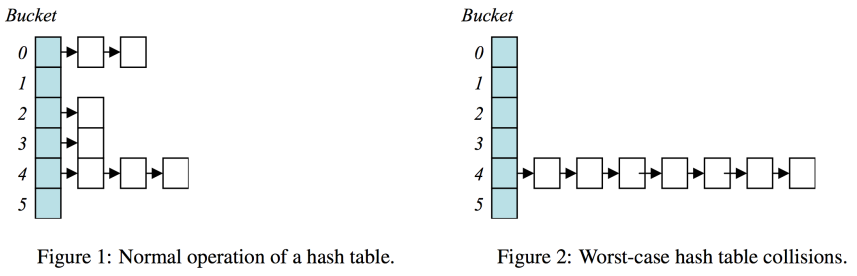
\includegraphics[width=0.5\linewidth]{figures/ddos_hash_collision}
	\caption{Hash table lookup: Collisions}
	\label{fig:ddoshashcollision}
\end{figure}

\subsubsection{Regular Expression Denial of Service (ReDoS)}

There are "malicious" inputs to certain regular expressions that take a very long time to evaluate. A server could become unresponsive when facing such a regex.\\
Example: input aaaaaa!@gmail.com to:\\
\texttt{([a-zA-Z0-9])(([\-.]+)?([a-zA-Z0-9]+))*(@){1}[a-z0-9]+[.]{1}(([a-z]{2,3})|([a-z]{2,3}[.]{1}[a-z]{2,3}))}

\subsection{Slowloris Attack}

Slowloris allows a single machine to take down another machine's web server with minimal bandwidth and side effects on unrelated services and ports.\\
\textbf{Basic idea:} Slowloris tries to keep many connections to the target web server open and hold them open as long as possible. Periodically, it will send subsequent HTTP headers, adding to - but never completing - the request. This will fill the maximum concurrent session pool of the server, eventually denying additional connection attempts from clients.\\

\textbf{Mitigation:}

\vspace{-\topsep}
\begin{itemize}
	\setlength{\itemsep}{0pt}
	\setlength{\parskip}{0pt}
	\item increase the maximum number of clients the webserver will allow
	\item limit the number of connection per srcIP
	\item put a lower bound on the transfer speed (might lose some customers with very slow internet), but this forces the attacker to spend at least some resources
	\item put an upper bound on the connection time (again, might lose some legitimate customers)
	\item setup reverse proxies, firewalls, load balancers or content switches
\end{itemize}
\vspace{-\topsep}

\subsection{DNS Reflection and Amplification Attack}

See section \ref{dns_ddos} for more information.\\

\textbf{Attack:} Attacker sends lots of UDP packets to a system whose replies are much larger than the requests (e.g. DNS, NTP, memcached) (amplification). Attacker further spoofs the srcIP to the victim's IP, such that the victim gets the large response traffic (reflection).

\vspace{-\topsep}
\begin{itemize}
	\setlength{\itemsep}{0pt}
	\setlength{\parskip}{0pt}
	\item Example: DNS is well-suited for this kind of attack: (1) DNS is over UTP (stateless protocol), which is fire-and-forget. (2) The srcIP can be spoofed. (3) DNS also is capable of generating a much larger response than query (e.g. dig ANY isc.org @x.x.x.x, 50x amplification).
\end{itemize}
\vspace{-\topsep}

\begin{figure}
	\centering
	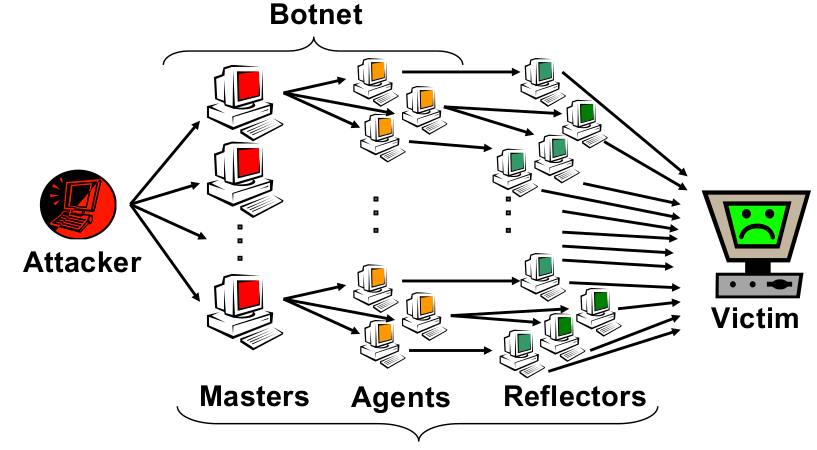
\includegraphics[width=0.4\linewidth]{figures/ddos_with_reflectors}
	\caption{Distributed DoS with Reflectors}
	\label{fig:ddoswithreflectors}
\end{figure}

Attackers can also use a botnet in addition to a normal amplification attack $\rightarrow$ \textit{distributed} denial of service attack (DDoS). Here multiple agents (bots) send the DNS request with the spoofed srcIP.

\newpage

\noindent\textbf{Key ingredients for reflection DOS / DDOS attacks:}

\vspace{-\topsep}
\begin{itemize}
	\setlength{\itemsep}{0pt}
	\setlength{\parskip}{0pt}
	\item Spoofing: Hide the origin and redirect replies to target
	\item Amplification: A small request generates a large response.
	\item Reflection: Combining source spoofing and amplification allows the 	abuse of third party services/protocols for powerful DOS attacks
	\item Open resolver: resolver that replies to any request
\end{itemize}
\vspace{-\topsep}

Any protocol / service with these attributes can be abused for a reflection attack.

\textbf{Mitigation:}

\vspace{-\topsep}
\begin{itemize}
	\setlength{\itemsep}{0pt}
	\setlength{\parskip}{0pt}
	\item Source IP verification: Reject packets with source addresses not reachable via the actual packet’s	path. This needs to be done in hosting and ISP environments. This is generally difficult to achieve. Some approaches try to correlate the srcIP with the TTL and check if this matches $\rightarrow$ this doesn't really work well, also the attacker could just match the TTL.
	\item Disable recursion on authoritative name servers
	\item Limit recursion to authorized clients
	\item Response Rate Limiting (RRL): Limit the number of responses to a client IP
\end{itemize}
\vspace{-\topsep}


\subsection{NTP Reflection and Amplification Attack}

Network Time Protocol (NTP) is used to synchronize all participating computers to within a few milliseconds of UTC. NTP is UDP based (port 123). NTP MONLIST obtains and prints an NTP server's monitor data: returns information of up to 600 clients the connected to the server (amplification factor of up to 143x is possible).\\
$\rightarrow$ spoofing \checkmark, amplification \checkmark, reflection \checkmark, open resolver \checkmark\\
$\rightarrow$ can be abused for (D)DoS attack!

\textbf{NTP-based DDoS Attack Recipe:}

\vspace{-\topsep}
\begin{enumerate}
	\setlength{\itemsep}{0pt}
	\setlength{\parskip}{0pt}
	\item Find vulnerable NTP servers (amplifiers), e.g., using nmap.
	\item Craft NTP MONLIST packet with src-address of the victim
	\item Send spoofed MONLIST requests to amplifiers
	\item ???
	\item Profit
\end{enumerate}
\vspace{-\topsep}

\textbf{Mitigation:}

\vspace{-\topsep}
\begin{itemize}
	\setlength{\itemsep}{0pt}
	\setlength{\parskip}{0pt}
	\item Server admins: Update NTP servers to version 4.2.8 (removes support for MONLIST)
	\item Network operators: Implement BCP-38 (ingress traffic filtering, see \ref{ip_spoofing_defense})
\end{itemize}
\vspace{-\topsep}

\newpage

\subsection{Shrew Attack}

Conventional bandwidth-based DoS requires sending high-rate attack traffic (like an elephant). Can we achieve the same effect by sending low-rate attack traffic (like a fierce shrew)? YES!\\

\textbf{Shrew DoS Attack:} Exploits TCP congestion control feature. Researchers discovered that if you send traffic during very short but specific amounts of time, you can completely disrupt TCP. This is due to TCP congestion control resending packets at multiple whole seconds granularity (1s, 2s, 4s, 8s, ...). By only creating congestion during these time periods 
the attacker forces TCP flows to repeatedly enter a retransmission timeout state by sending high-rate but short-duration bursts! We deny the bandwidth of legitimate TCP flows as it makes TCP believe there is a long-term congestion.\\

\textbf{Temporal lensing:} "multiple rounds simultaneous impact”. Use time as an additional amplification factor. Different paths have different transmission delays. An attacker can send packets at different times s.t. they \textit{all} arrive at the target \textit{at the same time}. So that a low-bandwidth source can also perform a shrew attack.

\subsection{IoT botnets}

IoT is expanding, more \& more devices go online. The curse of IoT is that devices are generally setup-and-forget and they are difficult and tedious to update which leads to many vulnerable devices (see section \ref{iot}).\\

IoT devices are ideal for DDoS botnets for a variety of reasons:

\vspace{-\topsep}
\begin{itemize}
	\setlength{\itemsep}{0pt}
	\setlength{\parskip}{0pt}
	\item IoT devices have less room for security features
	\item Developers are often less security focused when developing IoT software (compared to PC)
	\item re-use of default passwords \& people not changing their password
	\item no bandwidth limitation
\end{itemize}
\vspace{-\topsep}

Example: Mirai botnet, $10^6$ bots (mostly IP cameras), 1.3 Tbps against github (see \ref{mirai_botnet}).

\textbf{IoT botnet mitigation:}

\vspace{-\topsep}
\begin{itemize}
	\setlength{\itemsep}{0pt}
	\setlength{\parskip}{0pt}
	\item Patch: prioritize security and support automatic security updates
	\item Credentials: users need to change default credentials, manufacturers should not leave hard coded credentials in firmware or hardware
	\item Traffic monitoring: Service providers need to	actively monitor their network
\end{itemize}
\vspace{-\topsep}

\subsection{DDoS Ransoms}

Criminals threaten institutions such as banks that they are going to DDoS their services if they do not pay a certain amount. It's often unclear if the threat is real at all...\\
Banks often just pay since the potential damage can be much larger than the sums they have to pay (e.g. 25BTC $\approx$ 225k \$).

\subsection{General Countermeasures}

\begin{itemize}
	\setlength{\itemsep}{0pt}
	\setlength{\parskip}{0pt}
	\item Ingress filtering: Removes packets with illegitimate source IPs
	\item Computational puzzles: Slows down attacks, achieves per-computation fairness (e.g. this requires resources of attackers but is no problem for legit customers). Also: captchas slow down automation.
	\item Cloud- or ISP-based filtering: Delegates defense to cloud or ISP
	\item Network capabilities: Allows victim to block unwanted traffic closer to the source
	\item IP traceback:	Reveals the real source IPs of packets
\end{itemize}
\vspace{-\topsep}

\subsubsection{How to get 99.999\% uptime (\textless 5 min down/year)}

This is extremely difficult to achieve. A single BGP outage can take 3-5 minutes to reconfigure! Use (1) Redundancy: no single point of failure, over provision, multiple geographic locations, multiple independent internet connections, (2) Monitoring \& Rapid detection, (3) Failure resiliency: System can tolerate various temporary component failures.

\subsubsection{Long Term Monitoring}

Continuously gather data (bandwidth, packets, CPU, transaction), look at the time series. Monitoring is very important on a long term basis. Sometimes huge traffic can be legit (e.g. reddit hug of death, flash crowds, black friday,...). Perform long term monitoring to assess periodicity and peak periods/loads.

\subsubsection{Over Provisioning}

Plan bandwidth and resources to cover the majority of extreme peak loads. Consider peak loads under attack/ denial of service or during high demand periods (Black Friday, promotions,
sports events).

\subsection{In-network and Cloud-based DDoS	Mitigation Services}

\textit{Main point: DDoS is solved if you are very rich.}

So what is the problem? DDoS is essentially solved, Akamai and Cloudflare have invested so much in infrastructure that they can mitigate any DDoS attack. \textit{But:} these services are very expensive! It's essentially only for the rich. Also, you have to pay for a certain level of protection (i.e. how much bandwidth). Attacker could just send more and I'd be vulnerable again.

\subsubsection{Cloud-based DDoS Mitigation Service}

Cloud/CDN providers such as Akamai or Cloudflare offer DDoS mitigation. By changing BGP or DNS of web server, the traffic is redirected to the provider as a middle-man (e.g. use BGP anycast to have the same IP address at different places). Some provide Content Delivery Network (CDN) service to achieve diversion of traffic. This is today's state of the art.

\subsubsection{ISP-based DDoS Mitigation Service}

Upon detecting a DDoS attack, ISP redirects \textit{entire} traffic destined to victim to the scrubbing center, then send good traffic back to the destination. Scrubbing center keeps state for each connection (lots of machines) and uses Deep packet inspection (DPI) and connection pattern to filter malicious traffic. Parts of the detection algorithm is signature based (needs frequent updates).

\begin{figure}[b!]
	\centering
	\begin{subfigure}[t]{.5\textwidth}
		\centering
		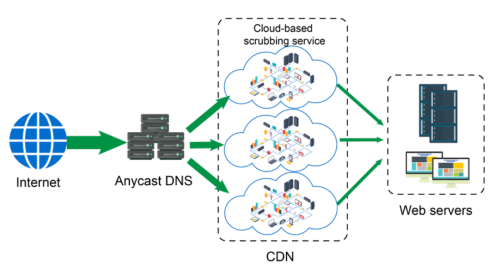
\includegraphics[width=0.7\linewidth]{figures/ddos_cloud_mitigation}
		\label{fig:ddos_cloud_mitigation}
		\caption{Cloud-based DDoS Mitigation Service}
	\end{subfigure}%
	\begin{subfigure}[t]{.5\textwidth}
		\centering
		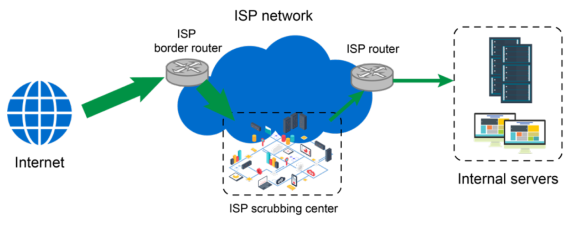
\includegraphics[width=0.9\linewidth]{figures/ddos_isp_mitigation}
		\label{fig:ddos_isp_mitigation}
		\caption{ISP-based DDoS Mitigation Service}
	\end{subfigure}
	\caption{}
\end{figure}

\subsubsection{Discussion: Cloud- or ISP-based Filtering}

\begin{itemize}
	\setlength{\itemsep}{0pt}
	\setlength{\parskip}{0pt}
	\item Cloud-based security provider can be easily bypassed: Because most cloud use DNS to redirect traffic, attackers can easily bypass the proxies if the victim’s IP is exposed.
	\item Privacy violation: E.g., Radware decrypts HTTPS and injects CAPTCHAs to client. An untrusted or compromised cloud could expose users’ sensitive data.
	\item Very limited destination traffic control
	\item High cost for small-, medium-size organizations
	\item Requires continuous subscription for fetching attack signatures
\end{itemize}
\vspace{-\topsep}

\subsection{Remotely Triggered Black Hole Filtering (RTBH)}

RTBH is a generic technique that can be used to mitigate volumetric DoS attacks - the offending traffic is simply dropped (black-holed) at the border routers of an AS. RTBH comes in two flavors, source-based and target-based.

\begin{itemize}
	\setlength{\itemsep}{0pt}
	\setlength{\parskip}{0pt}
	\item source-based RTBH: All traffic from attacker's subnet is dropped by target's ISP
	\item destination-based RTBH: All traffic to the target’s subnets is dropped by the target’s ISP\\
\end{itemize}
\vspace{-\topsep}

RTBH will drop traffic at the border routers, so that the traffic does not even enter the AS. The main solution is to sink all traffic that is destined to a particular placeholder IP address, chosen among an unused subnet. The subnet usually chosen is 192.0.2.0/24, technically reserved for testing purposes. Let’s say that we want all traffic destined to 192.0.2.1 to be dropped: we will then create the following static route. \texttt{ip route 192.0.2.1 255.255.255.255 null0}.\\
The RTBH will be triggered by an admin that will insert route updates that route traffic destined to the
attacked IP to the placeholder IP, 192.0.2.1 . These routes will then be propagated via iBGP to the edge routers, effectively making them send all the attack traffic to \texttt{null0}.

\subsection{FlowSpec (RFC5575)}

FlowSpec supports actions based of level 4 protocol matching. This could e.g. be used to mitigate a volumetric attack that exploits memcached (just block UDP port 11211 (memcached)).\\
But: The mitigation still (mostly) requires manual human intervention, all of your peers need to support FlowSpec, cannot distinguish attacks at levels \textgreater 4.

\subsection{Famous attacks}

\subsubsection[Github attack]{Github attack \footnote{\href{https://github.blog/2018-03-01-ddos-incident-report/}{https://github.blog/2018-03-01-ddos-incident-report/}}}

Github was attacked by a purely volumetric attack that exploited memcached and generated 1.3 Tbps. Github (who has its own AS, 36459) has connectivity through multiple providers - during the DDoS, they withdrew BGP announcements form all the providers but Akamai. This allowed Akamai to act as a shield for the attack: their infrastructure absorbed all of the load and filtered memchached traffic, only forwarding legitimate traffic to Github.

\subsubsection[“Great Cannon” browser-based DDoS]{“Great Cannon” browser-based DDoS \footnote{\href{https://citizenlab.ca/2015/04/chinas-great-cannon/}{https://citizenlab.ca/2015/04/chinas-great-cannon/}}}

Application-layer attack: Malicious JavaScript executed when users outside China visited sites
with Baidu’s user tracking code. All of the attack traffic was comprised of seemingly legitimate HTTP requests.

\newpage

\section{DDoS RIP}

\subsection{Next-generation attacks}

Both of these attacks haven't been seen in the wild yet but are theoretically possible.

\subsubsection{Coremelt attack}

Adversary controls many bots distributed across the Internet. Bots send traffic \textit{between each other}, thus all traffic they produce is legit traffic desired by the destination (destinations are bots). Traffic is not sent to a victim as in regular DDoS attacks. Thus, all defense methods discussed in section \ref{ddos} do not work here.\\
Adversary can exhaust bandwidth on victim link. As a result, the attack traffic exhausts bandwidth in per-flow fair sharing systems.

\subsubsection{Crossfire attack}

\textbf{Goal:} attacker wants to disconnect part of the internet from the rest.\\
Attacker detects some target links that connect a target region to the rest of the internet. Due to route optimization, few links are actually used to connect a
target region to rest of Internet. The attacker then overloads these specific target links by using a distributed bot army she controls. The bots communicate with target servers in/ near the target region and simply send TCP SYN packets. This can be enough to congest due to lots of target servers. This is hard to stop since only connection establish packets (TCP SYN) are sent.\\
\textbf{Result:} disconnect target region from remainder of Internet

\begin{figure}[hb]
	\centering
	\begin{subfigure}[t]{.5\textwidth}
		\centering
		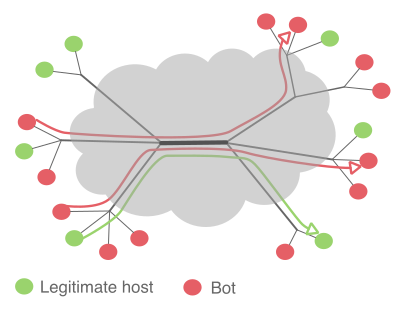
\includegraphics[width=0.8\linewidth]{figures/coremelt_attack}
		\label{fig:coremelt_attack}
		\caption{Coremelt Attack}
	\end{subfigure}%
	\begin{subfigure}[t]{.5\textwidth}
		\centering
		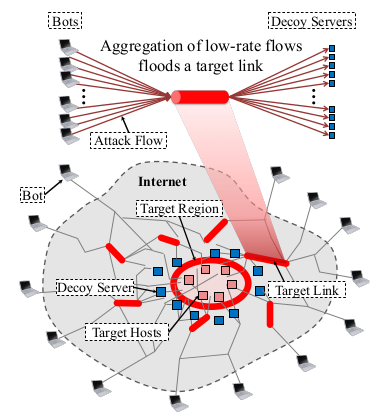
\includegraphics[width=0.6\linewidth]{figures/crossfire_attack}
		\label{fig:crossfire_attack}
		\caption{Crossfire attack}
	\end{subfigure}
	\caption{}
\end{figure}

\subsection{Next-generation defenses}

\subsubsection{SCION: Hidden paths}

AS does not announce a path to a core path server to the world, instead it keeps it secret. In SCION, we announce paths to the global path server (path server of a core AS) from where other entities can fetch the path. If we \textit{don't} announce a path to a global path server, other entities (and thus attackers) do not have a HOP field for it $\rightarrow$ packets would be dropped early if sent anyway over this path.
If for example some branch office wants to reach a central office via a hidden path, we need some rendez-vous service.\\

\textbf{Attack against hidden path:} if an attacker can obtain the hub field by catching a packet with the field, the attacker can then send on the hidden path. A hub field is valid for ca. 8 hours $\rightarrow$ this is rather long.\\

In conclusion, hidden paths are a rather weak DDoS defense.

\subsubsection{DRKey}

Idea: use a per-AS secret value to derive keys with an efficient Pseudo-Random Function (PRF). Every AS has a local secret from which different keys are derived $\rightarrow$ no need to fetch keys from memory, you can just rederive them in CPU.\\

\textbf{Example:} AS X creates a key for AS Y (s.t. AS Y can be source-authenticated when communicating with AS X) using secret value $SV_X$

\vspace{-\topsep}
\begin{itemize}
	\setlength{\itemsep}{0pt}
	\setlength{\parskip}{0pt}
	\item $K_{X\rightarrow Y} = PRF_{SV_X}("Y")$
	\item Intel AES-NI instructions enable PRF computation within 30 cycles, or 70 cycles for CMAC. \textit{Key computation is 3-5 times faster than DRAM key lookup!}
	\item Any entity in AS X knowing secret value $SV_X$ can derive $K_{X\rightarrow *}$
\end{itemize}
\vspace{-\topsep}

\textbf{Notation:} $K_{X\rightarrow Y}$: X can locally derive the key for Y (fast, based on a single local key $SV_X$) but on side of Y, you need to contact the local key server to fetch the key (slow). Arrow indicates direction of key derivation, not the direction of communication. Data flow is opposite to the key generation flow: AS Y uses $K_{X\rightarrow Y}$ for MACing data, and X checks those MACs. In this way, the burden of fetching the key (a slower operation) is on the
sender, while the receiver can always efficiently verify the data it receives.\\

\textbf{Key Server Infrastructure:}

Key servers that are deployed in each AS build backbone of key hierarchy. Responsible for key exchange, local key establishment and key management. After AS-level keys are established, symmetric keys for end hosts can be provided using key derivation. Keys can be used to provide source authenticity of packet without costly key exchange between communicating parties. Each host is required to contact their local key server.\\

\textbf{Key Hierarchy:} Key establishment using a multi-level key hierarchy using a one-way pseudo-random function. Whoever has the 0th level key can quickly derive all other keys (for its AS).

\vspace{-\topsep}
\begin{itemize}
	\setlength{\itemsep}{0pt}
	\setlength{\parskip}{0pt}
	\item \textbf{0th level:} per-AS local secret key (e.g. $SV_X$ for AS X). Represents basis of hierarchy and renewed frequently (e.g., daily)
	\item \textbf{1st-level:} key shared between ASes. AS uses 0th level key to derive symmetric key for other ASes (e.g. AS X derives $K_{X\rightarrow Y}$ for AS Y).
	\item \textbf{2nd-level:} key shared between internal host and external AS (e.g. AS X creates $K_{X\rightarrow Y:H_y}$ to source-authenticate host $H_y$ sending from within AS Y to AS X. Similarly, AS Y creates $K_{Y\rightarrow X:H_x}$ to source-authenticate host $H_x$ sending from within AS X to AS Y)
\end{itemize}
\vspace{-\topsep}

AS A creates key hierarchy from secret value A ($SV_A$) using a pseudo-random function (PRF): $K_{A\rightarrow B} = PRF_{SV_A}("B")$. Similarly, AS B creates key hierarchy based on $SV_B$.\\

\textbf{First-level DRKey:} Each AS has a key server with the 0th level key SV. An AS Y needs to fetch key $K_{X\rightarrow Y}$ from AS X in order to communicate with AS X. Key server in AS Y fetches $K_{X\rightarrow Y}$ from AS X through a secure channel set up based on AS certificates. Key server distributes local secret value SV to trusted infrastructure nodes inside same AS.\\
Insight: SV enables high-speed local key derivation of any other AS’ key.

\newpage

\begin{figure}
	\centering
	\includegraphics[width=0.7\linewidth]{figures/drkey_firstlevel_key_exchange}
	\caption{First-level Key Exchange. Secret value $SV_i$ for AS i, private key $K_i^{-1}$ for AS i. Public key $K_i$ for AS i. ASes send each other daily encrypted messages (asymmetric crypto).}
	\label{fig:drkeyfirstlevelkeyexchange}
\end{figure}

\textbf{Second-level DRKey:} apply PRF once more on AS-to-AS key to derive AS-to-Host symmetric key. AS X creates a key for host $H_y$ in AS Y:

\vspace{-\topsep}
\begin{itemize}
	\setlength{\itemsep}{0pt}
	\setlength{\parskip}{0pt}
	\item $K_{X\rightarrow Y} = PRF_{SV_X}("Y")$
	\item $K_{X\rightarrow Y:H_y} = PRF_{K_{X\rightarrow Y}}("H_y")$
\end{itemize}
\vspace{-\topsep}

Knowing secret value SV X any entity in AS X can derive $K_{X\rightarrow *:*}$. Knowing $K_{X\rightarrow Y}$, key server in AS Y can derive $K_{X\rightarrow Y:*}$. Host-to-Host keys $K_{X:*\rightarrow Y:*}$ can be similarly derived.\\

\textbf{DRKey use case: SCMP authentication}\\

SCMP instead of ICMP. Send an error when border router encounters error with a packet\\ $\rightarrow$ source-authenticate error message with DRKey. Assume Host H in AS A sends an SCMP message, and AS C, which receives this message, wants to authenticate it:

\vspace{-\topsep}
\begin{enumerate}
	\setlength{\itemsep}{0pt}
	\setlength{\parskip}{0pt}
	\item First-level Key Exchange: AS C has its local secret $SV_C$ . It uses $SV_C$ to generate the first
	level key $K_{C\rightarrow A} = PRF_{SV_C}("A")$. AS C securely sends $K_{C\rightarrow A}$ to AS A.
	
	\item Second-level Key Exchange: AS A generates a second-level key for H that can be used SCMP for source authentication by AS C, i.e., $K_{C\rightarrow A:H}^{SCMP} = PRF_{K_{C\rightarrow A}}("H|SCMP")$ and gives it to host H.
	
	\item Host H authenticates its ICMP message using $K_{C\rightarrow A:H}^{SCMP}$
	
	\item AS C dynamically recreates $K_{C\rightarrow A:H}^{SCMP}$ by retrieving the first-level key that it generated in Step 1 and computing the second-level key that AS A computed.
	
	\item Finally it verifies the authenticity of the message.
\end{enumerate}
\vspace{-\topsep}

\newpage

\subsubsection{EPIC (Every Packet Is Checked)}

\textbf{Goal:} Every router can source authenticate every packet in the internet with almost no overhead. Achieve per-packet source authentication, duplicate suppression, per-packet variable hop fields. Assumption: global time synchronization ($\pm$ 100 ms). EPIC can prevent attacks such as: (1) Malicious router replays packets or increases packet size. (2) Hop field MAC is brute forced and destination attacked until expiration time.\\

\textbf{EPIC level 1:} 

Current SCION hop field MAC: $MAC_{K_i}(TS||IgIF||EgIF||ExpT||\sigma_{i-1})$\\

TS: time beacon creation, ExpT: Expiration time, IgIF/EgIF: Ingress/Egress Interface,\\
T: time packet creation, $\sigma_{i-1}$: previous hop field MAC.\\

With EPIC, we have one additional level of indirection:

\vspace{-\topsep}
\begin{itemize}
	\setlength{\itemsep}{0pt}
	\setlength{\parskip}{0pt}
	\item $K_H = MAC_{K_i}(TS||IgIF||EgIF||ExpT||S_{i-1})$
	\item $S_i = H(K_H)$
	\item hop field MAC: $MAC_{K_H}(T||H(P))$
\end{itemize}
\vspace{-\topsep}

Hop key $K_H$ is distributed via beacon (PCB), $S_i$ is included in packet header. Result: every packet has unique hop field MAC, foiling brute force attacks on hop field MAC.\\

\textbf{EPIC level 2:}

Goal: achieve source authentication for every packet by including DRKey $K_{X\rightarrow Y:H}$ in hop field MAC. For host e in AS E, traversing AS X:

\vspace{-\topsep}
\begin{itemize}
	\setlength{\itemsep}{0pt}
	\setlength{\parskip}{0pt}
	\item $K_H = MAC_{K_i}(TS||IgIG||EgIF||ExpT||S_{i-1})$
	\item $S_i = H(K_H)$
	\item hop field MAC: $MAC_{K_H}(T||H(P)||K_{X \rightarrow E:e})$
\end{itemize}
\vspace{-\topsep}

Router in AS X can efficiently derive $K_{X \rightarrow E:e}$ (2 AES operations). Host e needs to fetch one key per AS traversed from local certificate server. Result: efficient per-packet per-hop source authentication! (5 AES op).


\subsubsection{PISKES}

PISKES uses DRKey to authenticate packets coming to a server. For every host sending a packet, derive the key locally and authenticate packet.\\
Client c in AS C fetches DRKey $K_{S \rightarrow C:c}$ from local certificate server. Server s in AS S can locally derive
DRKey and verify packet. Throughput is only slightly worse (0.2\% less for 128B packet, 15\% worse for 64B packet).

\subsubsection{History-based filtering}\

\textbf{Basic idea (omitting details)}: create a list of ASes that you communicate with and through monitoring, set a number of packets you allow these ASes to have in a given time period. Under a DDoS attack, you then filter based on ASes $\rightarrow$ only hosts from the AS with the attacker in it are affected.

\newpage

\subsubsection{COLIBRI}

Key ideas:

\vspace{-\topsep}
\begin{itemize}
	\setlength{\itemsep}{0pt}
	\setlength{\parskip}{0pt}
	\item Admission control: possible with DRKey
	\item Resource allocation: who should obtain some amount of resource $\rightarrow$ difficult to decide. COLIBRI wants two-tier reservation (tier-1: between ASes, tier-2: between end-hosts) and fairness (per-neighbor AS fairness).
	\item Traffic policing: who sends too much? Designed for scalability. Two layer model: at edge and at core.
	\item Traffic monitoring: per neighbor based traffic shaping. Designed for scalability. Two layer model: at edge and at core.
\end{itemize}
\vspace{-\topsep}

\textbf{Link BW Decomposition:}

\vspace{-\topsep}
\begin{itemize}
	\setlength{\itemsep}{0pt}
	\setlength{\parskip}{0pt}
	\item Bandwidth is reserved for \textit{segment reservations} (\textcolor{red}{shown in red}) (longterm)
	\item \textit{End-to-end} path reservation is created from multiple segment reservations \\
	(\textcolor{green}{shown in green})
	\item Remaining bandwidth (non-reserved or non-utilized) can be used for \textit{best-effort traffic} (\textcolor{blue}{shown in blue})
\end{itemize}
\vspace{-\topsep}

\textbf{Segment Reservation:}

Reservation on SCION path segment is initiated by the source AS of each path segment. Bandwidth class indicates the guaranteed and maximum bandwidth. Maximum validity period 5 minutes.\\
Example: ID A-42 allocate(min:10, max:20), AS A: max:20, alloc 20, AS B: max 15, alloc 15, AS C: max 18, alloc 15

\begin{figure}[hb]
	\centering
	\begin{subfigure}[t]{.5\textwidth}
		\centering
		\includegraphics[width=0.4\linewidth]{figures/colibri_linkbw_decomp}
		\label{fig:colibri_linkbw_decomp}
		\caption{Link BW Decomposition}
	\end{subfigure}%
	\begin{subfigure}[t]{.5\textwidth}
		\centering
		\includegraphics[width=0.6\linewidth]{figures/colibri_segment_reservation}
		\label{fig:colibri_segment_reservation}
		\caption{Segment Reservation}
	\end{subfigure}
	\caption{}
\end{figure}

\textbf{Admission Algorithm: Properties}

\vspace{-\topsep}
\begin{itemize}
	\setlength{\itemsep}{0pt}
	\setlength{\parskip}{0pt}
	\item Algorithm guarantees that no set of AS can reserve an "un-proportional" amount of bandwidth trough one link. In traditional internet, attacker can create malicious tree of ASes and claim each AS requests traffic. This does not work here.
	\item Algorithm guarantees that no AS can congest a link by reserving through multiple paths. In SCION paths are visible. An AS can realize when someone enters over multiple paths.
\end{itemize}
\vspace{-\topsep}

\textbf{Need for Monitoring:}

Misbehaving end host might exceed their reserved bandwidth and disrupt the network. Each Edge AS is accountable for its hosts and is required to perform per-flow (stateful) policing. At the edge, we can do per-flow monitoring. In the core, we need probabilistic monitoring.

\newpage

\textbf{Attacks:} Legacy traffic could be dangerous since an attacker could simply congest a link using legacy IPv4/IPv6 traffic and prevent SCION communication.\\
\textbf{Solution}: use of IP prioritization/ queuing: Reserve QoS classes for SCION traffic and configure prioritization on each switch/ router to reserve bandwidth for SCION.

\subsection{Conclusion}

Colibri allows hosts to reserve end to end paths between each other with guaranteed bandwidth. This solves the DDoS problem as the legitimate path is guaranteed at least some bandwidth. In order to reserve a path, first each segment needs to be reserved by the source AS, and then these reserved segments are used to exchange packets to set up the whole e2e path reservation. Every requesting host can request a certain bandwidth, but the guaranteed BW is assigned with a fairness algorithm, so each flow gets at least a slow path, but never interruption of the link.

\vspace{-\topsep}
\begin{itemize}
	\setlength{\itemsep}{0pt}
	\setlength{\parskip}{0pt}
	\item Server-based attack: solved by per-packet authentication, duplicate suppression, and history-based filtering
	\item Volumetric network congestion: solved by combination of systems:
	\begin{itemize}
		\item Reservation of bandwidth with availability of non-negligible BW amount (COLIBRI)
		\item Even on-path routers cannot cheat (EPIC)
	\end{itemize}

\end{itemize}
\vspace{-\topsep}

\label{lastpage} % this must stay here
\clearpage
\addcontentsline{toc}{section}{References}
\bibliographystyle{acm}
\bibliography{refs}

\clearpage
\appendix
\pagenumbering{Roman}

\end{document}
